\chapter{Results and Discussion}\label{ResultsDiscussion}

This chapter presents the results from the experiments described in the \ref{Experiments} Experiments chapter. These outcomes are organized in the following sections: ``\ref{FluidSegmentation} Fluid Segmentation'', ``\ref{IntermediateSliceSynthesis} Intermediate Slice Synthesis'', and ``\ref{FluidVolumeEstimation} Fluid Volume Estimation''. After showing the results from the experiments, the factors influencing them are discussed, while providing visual examples of the models' performances. The results are also compared with other similar approaches in literature, while explaining how these different methods lead to different results.

\section{Fluid Segmentation}\label{FluidSegmentation}
In this section, the results from the experiments performed in multi-class fluid segmentation are shown. This includes all the runs made in \ref{Experiment1} Experiment 1 and \ref{Experiment2} Experiment 2. In these sections, the resulting Dice coefficients are displayed in tables. Each value corresponds to the mean Dice coefficient computed across all slices present in the validation OCT volumes. The results are shown for each fluid (IRF, SRF, and PED) both grouped by vendor and across all vendors. There is also a column that contains the Dice coefficient when considering all the fluids as a single binary label. Unless specified otherwise, the Dice coefficient calculated for a fluid considers all the slices and not just those that contain the specified fluid and the values highlighted in bold are the best values obtained in each column. 
\par
These values are presented for each run, which follows the conditions described in the \ref{FluidSegmentation} Fluid Segmentation section. Every four runs that are completed using a different validation fold but follow the same conditions are grouped in a single row, by calculating their mean (row ``Set''). From the 5-fold split, fold 1 was reserved, while the remaining four (0, 2, 3, and 4) are used in training and validation. The fold selected for validation in each run appears in the table's validation fold (``VF'') column. For example, if the fold in the ``VF'' column is 2, then the folds used in training were 0, 3, and 4.
\par
In the following subsections, images displaying the segmentation performed by the models and the respective GT are shown. In these masks, IRF is represented in red, SRF in green, and PED in blue.

\subsection{Experiment 1 - Fluid Segmentation Using Multi-class U-Net}

\subsubsection{Experiment 1.1 - Random Patch Extraction}

The results from the first experiment performed, Experiment 1.1, are shown in Table \ref{tab:Experiment1.1Results}. In this experiment, for each validation fold, two runs were made, while keeping the same conditions. The only difference is the input data: as it is extracted randomly, as described in \ref{Methods} Materials and Methods, it is different for every run. 

\begin{table*}[!ht]
	\caption{Dice scores for every vendor and fluid for the runs done in Experiment 1.1. The conditions were the same for both sets except the extracted patches, which are different in every run due to the random patch extraction method used.}
	\centering
	\resizebox{\textwidth}{!}{\begin{tabular}{|c|c|ccc|ccc|ccc|c|c|c|c|}
		\hline
		% Headers
		\multirow{2}{*}{\textbf{Runs}} & 
		\multirow{2}{*}{\textbf{VF}} & 
		\multicolumn{3}{c|}{\textbf{Cirrus}} & 
		\multicolumn{3}{c|}{\textbf{Spectralis}} & 
		\multicolumn{3}{c|}{\textbf{Topcon}} & 
		\multicolumn{1}{c|}{\multirow{2}{*}{\textbf{IRF}}} & 
		\multirow{2}{*}{\textbf{SRF}} & 
		\multirow{2}{*}{\textbf{PED}} & 
		\multirow{2}{*}{\textbf{Fluid}} \\ \cline{3-11} & &
		\multicolumn{1}{c}{\textbf{IRF}} & 
		\multicolumn{1}{c}{\textbf{SRF}} & 
		\textbf{\textbf{PED}} & 
		\multicolumn{1}{c}{\textbf{IRF}} & 
		\multicolumn{1}{c}{\textbf{SRF}} & 
		\textbf{PED} & 
		\textbf{IRF} & 
		\textbf{SRF} & 
		\textbf{PED} & 
		\multicolumn{1}{c|}{} & & & \\ 
		
		\hline
		
		\textbf{Run 1} & 2 & \multicolumn{1}{c|}{0.138} & \multicolumn{1}{c|}{0.089} & 0.072 & \multicolumn{1}{c|}{0.255} & \multicolumn{1}{c|}{0.331} & 0.163
		& \multicolumn{1}{c|}{0.259} & \multicolumn{1}{c|}{0.446} & 0.056 & 0.200 & 0.254 & 0.083 & 0.163 \\
		
		\textbf{Run 2} & 3 & \multicolumn{1}{c|}{0.138} & \multicolumn{1}{c|}{0.290} & 0.236 & \multicolumn{1}{c|}{0.264} & \multicolumn{1}{c|}{0.670} & 0.652 & \multicolumn{1}{c|}{0.389} & \multicolumn{1}{c|}{0.532} & 0.284 & 0.252 & 0.445 & 0.327 & 0.303 \\
		
		\textbf{Run 3} & 4 & \multicolumn{1}{c|}{0.209} & \multicolumn{1}{c|}{0.158} & 0.024 & \multicolumn{1}{c|}{0.255} & \multicolumn{1}{c|}{0.451} & 0.310 & \multicolumn{1}{c|}{0.286} & \multicolumn{1}{c|}{0.595} & 0.151 & 0.249 & 0.386 & 0.117 & 0.173 \\ 
		
		\textbf{Run 4} & 0 & \multicolumn{1}{c|}{0.166} & \multicolumn{1}{c|}{0.179} & 0.041 & \multicolumn{1}{c|}{0.307} & \multicolumn{1}{c|}{0.343} & 0.243 & \multicolumn{1}{c|}{0.371} & \multicolumn{1}{c|}{0.376} & 0.052 & 0.266 & 0.280 & 0.081 & 0.165 \\ 
		
		\hline
	
		\textbf{Set 1} & - & \multicolumn{1}{c|}{0.16} & \multicolumn{1}{c|}{0.18} & 0.09 & \multicolumn{1}{c|}{0.27} & \multicolumn{1}{c|}{0.45} & 0.34 & \multicolumn{1}{c|}{0.33} & \multicolumn{1}{c|}{0.49} & 0.14 & 0.24 & 0.34 & 0.15 & 0.20 \\ 
	
		\hline
		\hline
	
		\textbf{Run 5} & 2 & \multicolumn{1}{c|}{0.106} & \multicolumn{1}{c|}{0.152} & 0.085 & \multicolumn{1}{c|}{0.290} & \multicolumn{1}{c|}{0.406} & 0.256 & \multicolumn{1}{c|}{0.433} & \multicolumn{1}{c|}{0.443} & 0.065 & 0.250 & 0.296 & 0.110 & 0.175 \\
		
		\textbf{Run 6} & 3 & \multicolumn{1}{c|}{0.370} & \multicolumn{1}{c|}{\textbf{0.297}} & 0.454 & \multicolumn{1}{c|}{\textbf{0.410}} & \multicolumn{1}{c|}{\textbf{0.735}} & \textbf{0.673} & \multicolumn{1}{c|}{0.205} & \multicolumn{1}{c|}{\textbf{0.821}} & \textbf{0.672} & 0.317 & \textbf{0.566} & 0.572 & 0.299 \\
		
		\textbf{Run 7} & 4 & \multicolumn{1}{c|}{\textbf{0.590}} & \multicolumn{1}{c|}{0.265} & \textbf{0.666} & \multicolumn{1}{c|}{0.296} & \multicolumn{1}{c|}{0.372} & 0.498 & \multicolumn{1}{c|}{\textbf{0.687}} & \multicolumn{1}{c|}{0.683} & 0.555 & \textbf{0.593} & 0.460 & \textbf{0.596} & \textbf{0.420} \\ 
		
		\textbf{Run 8} & 0 & \multicolumn{1}{c|}{0.321} & \multicolumn{1}{c|}{0.259} & 0.067 & \multicolumn{1}{c|}{0.352} & \multicolumn{1}{c|}{0.514} & 0.467 & \multicolumn{1}{c|}{0.410} & \multicolumn{1}{c|}{0.610} & 0.152 & 0.249 & 0.386 & 0.117 & 0.173 \\ 
		
		\hline
		
		\textbf{Set 2} & - & \multicolumn{1}{c|}{\textbf{0.35}} & \multicolumn{1}{c|}{\textbf{0.24}} & \textbf{0.32} & \multicolumn{1}{c|}{\textbf{0.34}} & \multicolumn{1}{c|}{\textbf{0.51}} & \textbf{0.47} & \multicolumn{1}{c|}{\textbf{0.43}} & \multicolumn{1}{c|}{\textbf{0.64}} & \textbf{0.36} & \textbf{0.38} & \textbf{0.44} & \textbf{0.36} & \textbf{0.27} \\ 
	
		\hline

	\end{tabular}}
	\label{tab:Experiment1.1Results}
\end{table*}

By looking at the table, a few conclusions can be drawn. First, the difference in performance between runs using the same training OCT volumes is evident. Despite some values being similar for the same training volumes, this trend becomes evident when looking at the mean values in the rows ``Set'', where a significant difference is noted, especially in the Cirrus vendor and the PED fluid. It is also evident that some VFs are more consistent than others. For example, for different extracted patches, the models evaluated on validation fold 2 and validation fold 0 presented similar results, while those evaluated in validation fold 3 showed significant differences when the input patches were changed.
\par
The second conclusion is that, overall, the models are not performing well, as the Dice results are low for every VF. These values are specially low in Cirrus, but better both in Spectralis, and Topcon. One of the reasons the model performed so poorly is due to the input it was receiving. Most of the extracted patches do not capture the transitions from background to retina and from retina to the choroid due to the small patch size. These transitions are of great importance in fluid segmentation in OCT scans since they represent, among other concepts, the boundaries of the region where fluid can appear. In case the model does not understand these anatomic boundaries, segmentation can be performed outside the retina, which worsens the Dice coefficient.
\par
Despite the performances not being good in every vendor, it is worse in Cirrus. In the literature, it is common to see worse performances in the images obtained with Cirrus and Topcon due to the larger presence of speckle noise in them. However, the poor performances observed in the Cirrus device were due to the size of the patches extracted from its B-scans. The B-scans in these volumes present a larger vertical resolution than those obtained with Topcon and Spectralis devices. Therefore, when extracting a patch of the same size across all devices, each patch from a Cirrus scan captures a smaller area of the retina. This translates to an worse understanding of the transition between background and retina and between retina and choroid, as shown in Figure \ref{fig:CirrusPatchExample}, ultimately leading to the oversegmentation beyond the retina.

\begin{figure}[!ht]
	\centering
	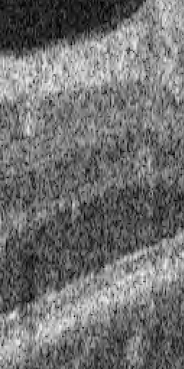
\includegraphics[width=0.18\linewidth]{figures/CirrusPatchExample.png}
	\caption{Example of a patch extracted from a Cirrus OCT volume used in Experiment 1.1. In this patch, while the background is noticeable due to its darker shade, the choroid is harder to be identified by an observer (or a model) due to the lack of context.}
	\label{fig:CirrusPatchExample}
\end{figure}

In Figure \ref{fig:Experiment11Segmentation}, it is shown a segmentation performed by the model trained in Run 1. In this figure it becomes evident that the model learned which areas can be segmented inside the retina, but does not understand how to handle the regions further away. For example, in the area significantly above the retina, the background is labeled as SRF. However, the background region closer to the retina is not so frequently labeled as any fluid, since it appears in the patches input to the model. The same problem occurs with the oversegmentation of PED in the choroid region, which does not appear in the input patches significantly. The fact that the patches are extracted exclusively from the ROI makes the model more prone to misclassify the background regions, as it did not see any patch that contained solely background.
\par
Oversegmentation beyond the retinal bounds is not exclusive to the Cirrus volumes, as it also appears in the OCT scans from other vendors. This suggests that the issue is primarily due to the small patch size and lack of background representitivity in the inputs rather than just the smaller retinal area captured in Cirrus patches, despite this amplifying the problem. 
\par
In the same figure, it is seen that the model has not learned the anatomical relationships between fluids, since it segmented IRF and PED close to each other. This occurs because the model has not learned the relationship between the retinal landmarks and the fluid types due to the small sized inputs.

\begin{figure}[!ht]
	\centering
	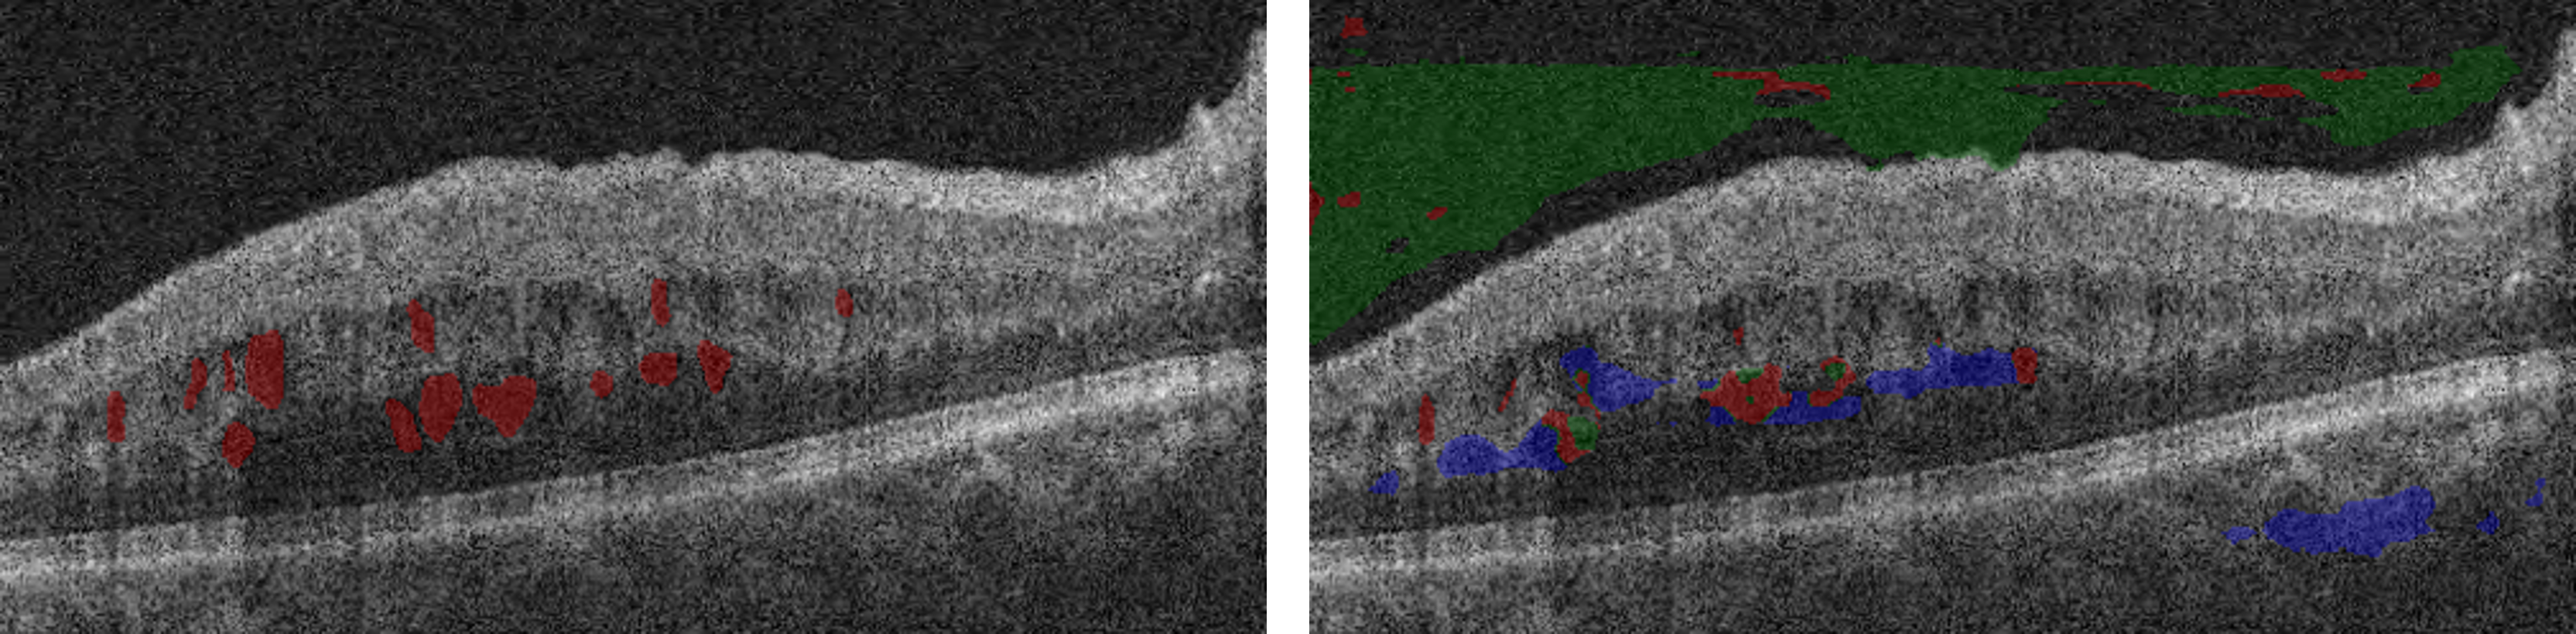
\includegraphics[width=1.0\linewidth]{figures/Experiment11Segmentation.png}
	\caption{Example of a poor segmentation made by the model trained in Run 1 (right). In the left, the GT mask for the same image is shown.}
	\label{fig:Experiment11Segmentation}
\end{figure}

\subsubsection{Experiment 1.2 - Large Patch Extraction}

The resulting Dice coefficient values obtained in Experiment 1.2, where patches of shape 496 $\times$ 512 were used, are shown in Table \ref{tab:Experiment1.2Results}.

\begin{table*}[!ht]
	\caption{Dice scores for every vendor and fluid for the runs done in Experiment 1.2.}
	\centering
	\resizebox{\textwidth}{!}{\begin{tabular}{|c|c|ccc|ccc|ccc|c|c|c|c|}
		\hline
		% Headers
		\multirow{2}{*}{\textbf{Runs}} & 
		\multirow{2}{*}{\textbf{VF}} & 
		\multicolumn{3}{c|}{\textbf{Cirrus}} & 
		\multicolumn{3}{c|}{\textbf{Spectralis}} & 
		\multicolumn{3}{c|}{\textbf{Topcon}} & 
		\multicolumn{1}{c|}{\multirow{2}{*}{\textbf{IRF}}} & 
		\multirow{2}{*}{\textbf{SRF}} & 
		\multirow{2}{*}{\textbf{PED}} & 
		\multirow{2}{*}{\textbf{Fluid}} \\ \cline{3-11} & &
		\multicolumn{1}{c}{\textbf{IRF}} & 
		\multicolumn{1}{c}{\textbf{SRF}} & 
		\textbf{\textbf{PED}} & 
		\multicolumn{1}{c}{\textbf{IRF}} & 
		\multicolumn{1}{c}{\textbf{SRF}} & 
		\textbf{PED} & 
		\textbf{IRF} & 
		\textbf{SRF} & 
		\textbf{PED} & 
		\multicolumn{1}{c|}{} & & & \\ 
			
		\hline
		
		\textbf{Run 9} & 2 & \multicolumn{1}{c|}{0.291} & \multicolumn{1}{c|}{0.450} & 0.281 & \multicolumn{1}{c|}{0.472} & \multicolumn{1}{c|}{0.638} & 0.394 & \multicolumn{1}{c|}{0.505} & \multicolumn{1}{c|}{0.647} & 0.573 & 0.396 & 0.551 & 0.400 & 0.393 \\

		
		\textbf{Run 10} & 3 & \multicolumn{1}{c|}{\textbf{0.586}} & \multicolumn{1}{c|}{\textbf{0.619}} & \textbf{0.727} & \multicolumn{1}{c|}{0.482} & \multicolumn{1}{c|}{\textbf{0.780}} & \textbf{0.698} & \multicolumn{1}{c|}{\textbf{0.749}} & \multicolumn{1}{c|}{\textbf{0.793}} & \textbf{0.788} & \textbf{0.627} & \textbf{0.711} & \textbf{0.744} & \textbf{0.667} \\

		
		\textbf{Run 11} & 4 & \multicolumn{1}{c|}{0.281} & \multicolumn{1}{c|}{0.453} & 0.415 & \multicolumn{1}{c|}{0.429} & \multicolumn{1}{c|}{0.503} & 0.322 & \multicolumn{1}{c|}{0.228} & \multicolumn{1}{c|}{0.532} & 0.324 & 0.278 & 0.494 & 0.363 & 0.296 \\
		
		\textbf{Run 12} & 0 & \multicolumn{1}{c|}{0.242} & \multicolumn{1}{c|}{0.334} & 0.336 & \multicolumn{1}{c|}{\textbf{0.551}} & \multicolumn{1}{c|}{0.564} & 0.423 & \multicolumn{1}{c|}{0.321} & \multicolumn{1}{c|}{0.643} & 0.407 & 0.325 & 0.488 & 0.377 & 0.339 \\
		
		\hline
		
		\textbf{Set 3} & - & \multicolumn{1}{c|}{0.35} & \multicolumn{1}{c|}{0.46} & 0.44 & \multicolumn{1}{c|}{0.48} & \multicolumn{1}{c|}{0.62} & 0.46 & \multicolumn{1}{c|}{0.45} & \multicolumn{1}{c|}{0.65} & 0.52 & 0.41 & 0.56 & 0.47 & 0.42 \\
		
		\hline
		\hline
		
		\textbf{Set 2} & - & \multicolumn{1}{c|}{\textbf{0.35}} & \multicolumn{1}{c|}{\textbf{0.24}} & \textbf{0.32} & \multicolumn{1}{c|}{\textbf{0.34}} & \multicolumn{1}{c|}{\textbf{0.51}} & \textbf{0.47} & \multicolumn{1}{c|}{\textbf{0.43}} & \multicolumn{1}{c|}{\textbf{0.64}} & \textbf{0.36} & \textbf{0.38} & \textbf{0.44} & \textbf{0.36} & \textbf{0.27} \\ 
		
		\hline
					
	\end{tabular}}
	\label{tab:Experiment1.2Results}
\end{table*}

The information resumed in this table allows the comparison between the performance in models that used smaller patches in Experiment 1.1 with those that used larger patches in this Experiment.
\par
By comparing the ``Set'' rows, it becomes evident an overall increase in performance when using larger patches. In fact, it is observed an increase in almost all the mean values when compared to the best performing set in Experiment 1.1. This increase is larger than one decimal point in some columns, and the largest improvements occur in the volumes obtained using the Cirrus device and when segmenting SRF or PED.
\par
The improvement in performance in Cirrus devices can be explained with the more contextual information given. In Experiment 1.1, the Cirrus patches input to the model were not big enough for the network to capture and understand the retinal borders or the relationship between them and the fluids, and the networks were trained with the small representation of background, thus leading to oversegmentation beyond the retina, as explained. In Experiment 1.2, as the same patch covers the retinal layer and the background simultaneously, the model has learned to not segment beyond the retina. In Figure \ref{fig:BigPatchesSegmentationCirrus}, the B-scan shown in Figure \ref{fig:Experiment11Segmentation}, is segmented by the model trained in Run 9 and it is possible to see that the labeling of the background as fluid is no longer happening.
\par 
This also partially justifies the significant improvement in the SRF and PED Dice coefficient. By providing inputs with enough context, the model is no longer segmenting these fluids outside the retina. However, in Figure \ref{fig:BigPatchesSegmentationCirrus} it is also seen that the model is no longer confusing the fluids in the retina, as it no longer segments the PED close to the IRF. This further justifies that the model is learning the anatomical references associated with PED, as confirmed in Figure \ref{fig:BigPatchesSegmentationTopcon}.
\par
Lastly, it is important to note that the IRF did not improve as much as the other fluids. This happens because the input patches in Experiment 1.1 where extracted mainly from the retina, providing all the anatomical context needed for the IRF segmentation. By training the model with larger patches, its attention to the finer details is reduced, therefore not producing fine and detailed segmentations in smaller fluid regions.
\par
In Figure \ref{fig:BigPatchesSegmentationTopcon}, it is seen that the model confuses the choroid with the retina, as it labels parts of that region as IRF and PED. The likely cause for this confusion is that the input patches are often cropped in the middle of the retinal layer (as illustrated in Figure \ref{fig:BigPatchExtraction}), which leads to the model not understanding the position of the choroid relative to the retina. This inaccurate IRF and PED segmentation is probably based on the visual resemblance between the structures seen in the choroid and the fluid regions in the retina. This indicates that the model does not know the location of the choroid.

\begin{figure}[!ht]
	\centering
	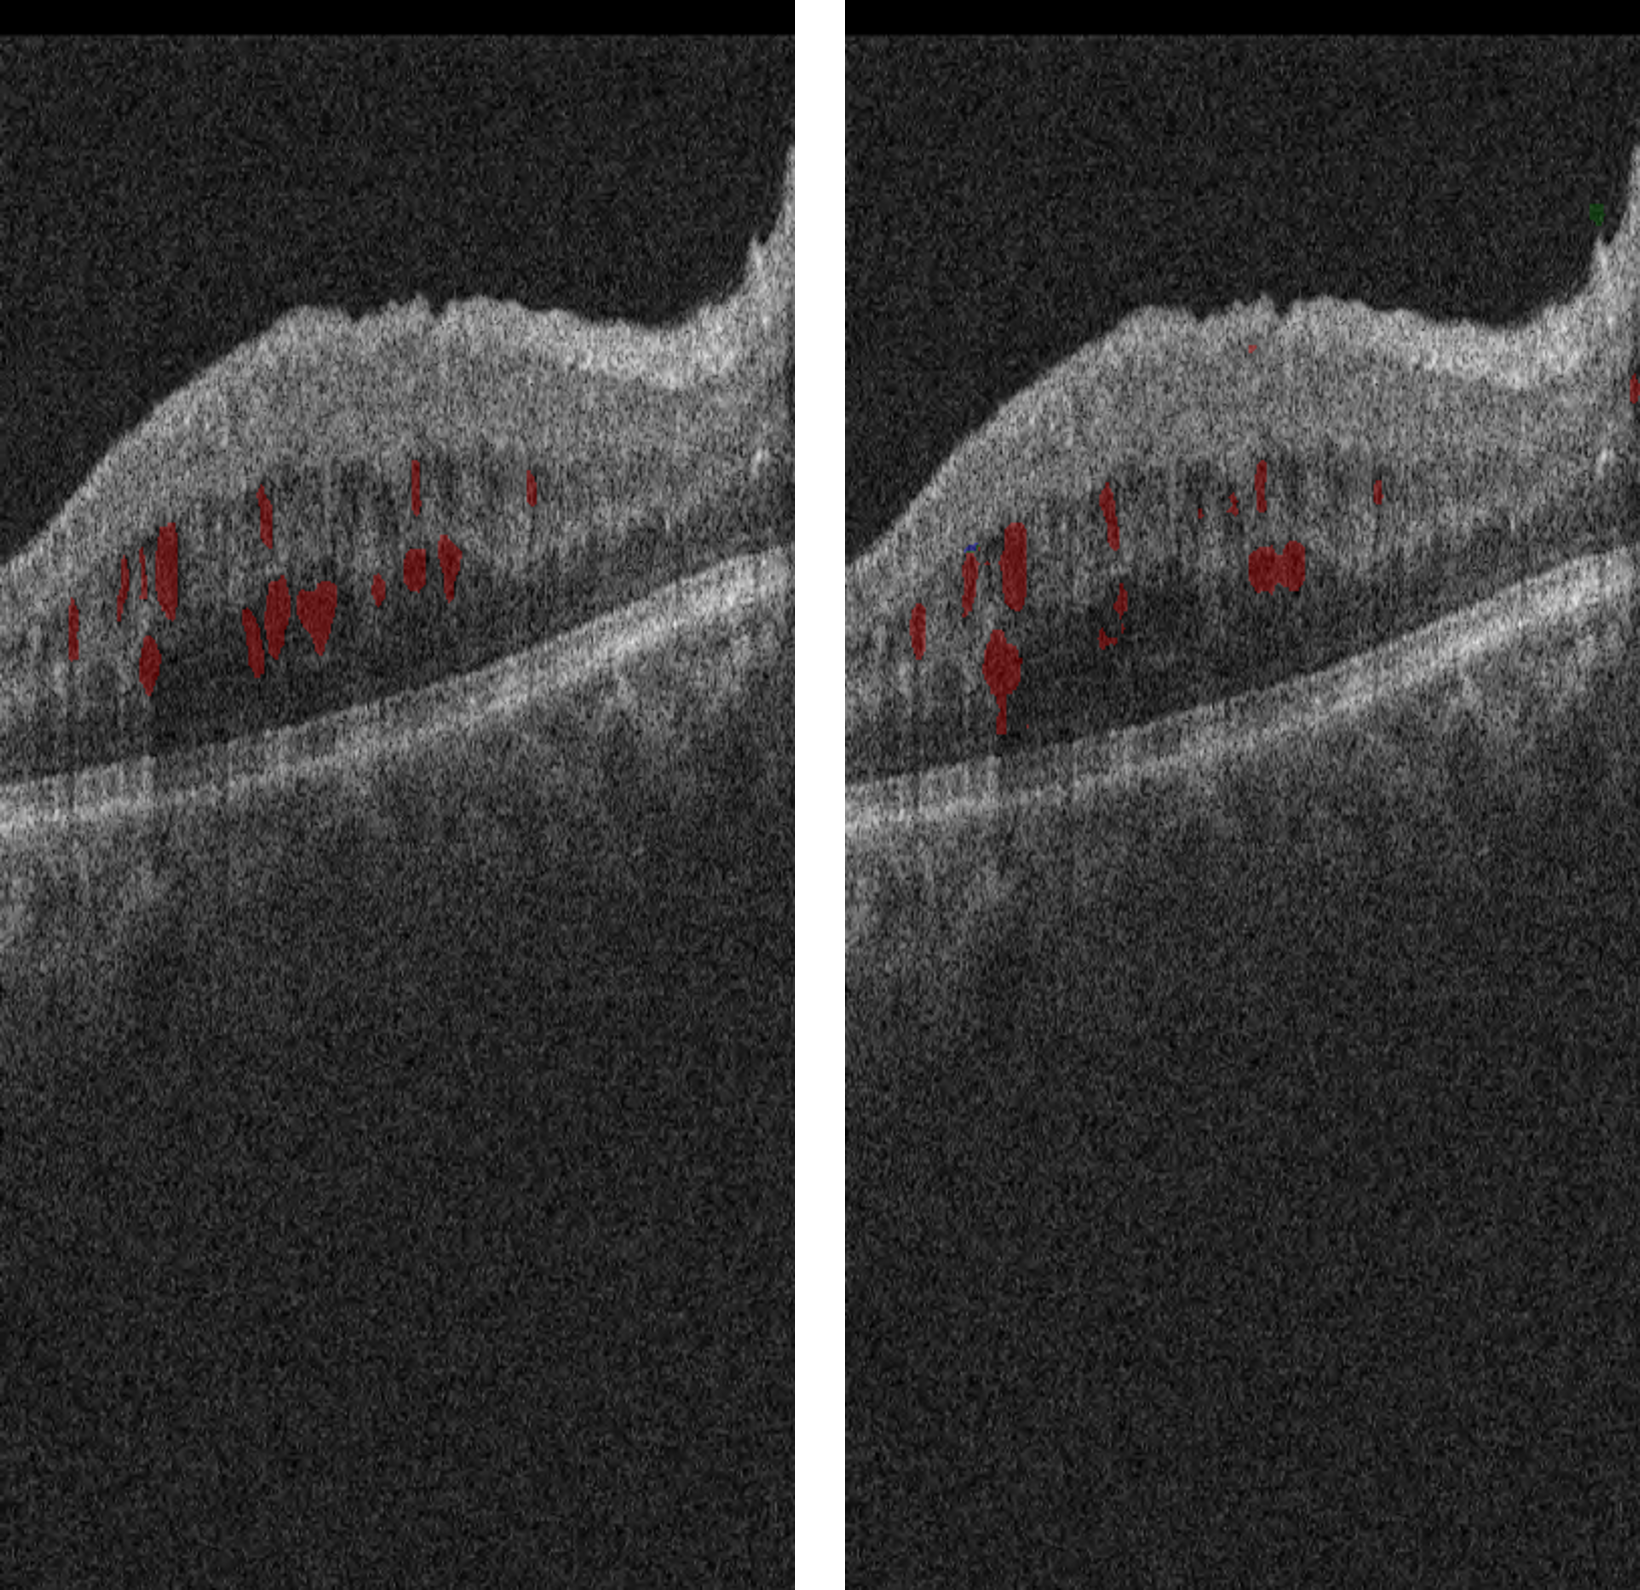
\includegraphics[width=0.5\linewidth]{figures/BigPatchSegmentationCirrus.png}
	\caption{Example of the segmentation done by the model trained in Run 9 (right) and its respective GT mask (left). The B-scan segmented is the same as in Figure \ref{fig:Experiment11Segmentation}.}
	\label{fig:BigPatchesSegmentationCirrus}
\end{figure}

\begin{figure}[!ht]
	\centering
	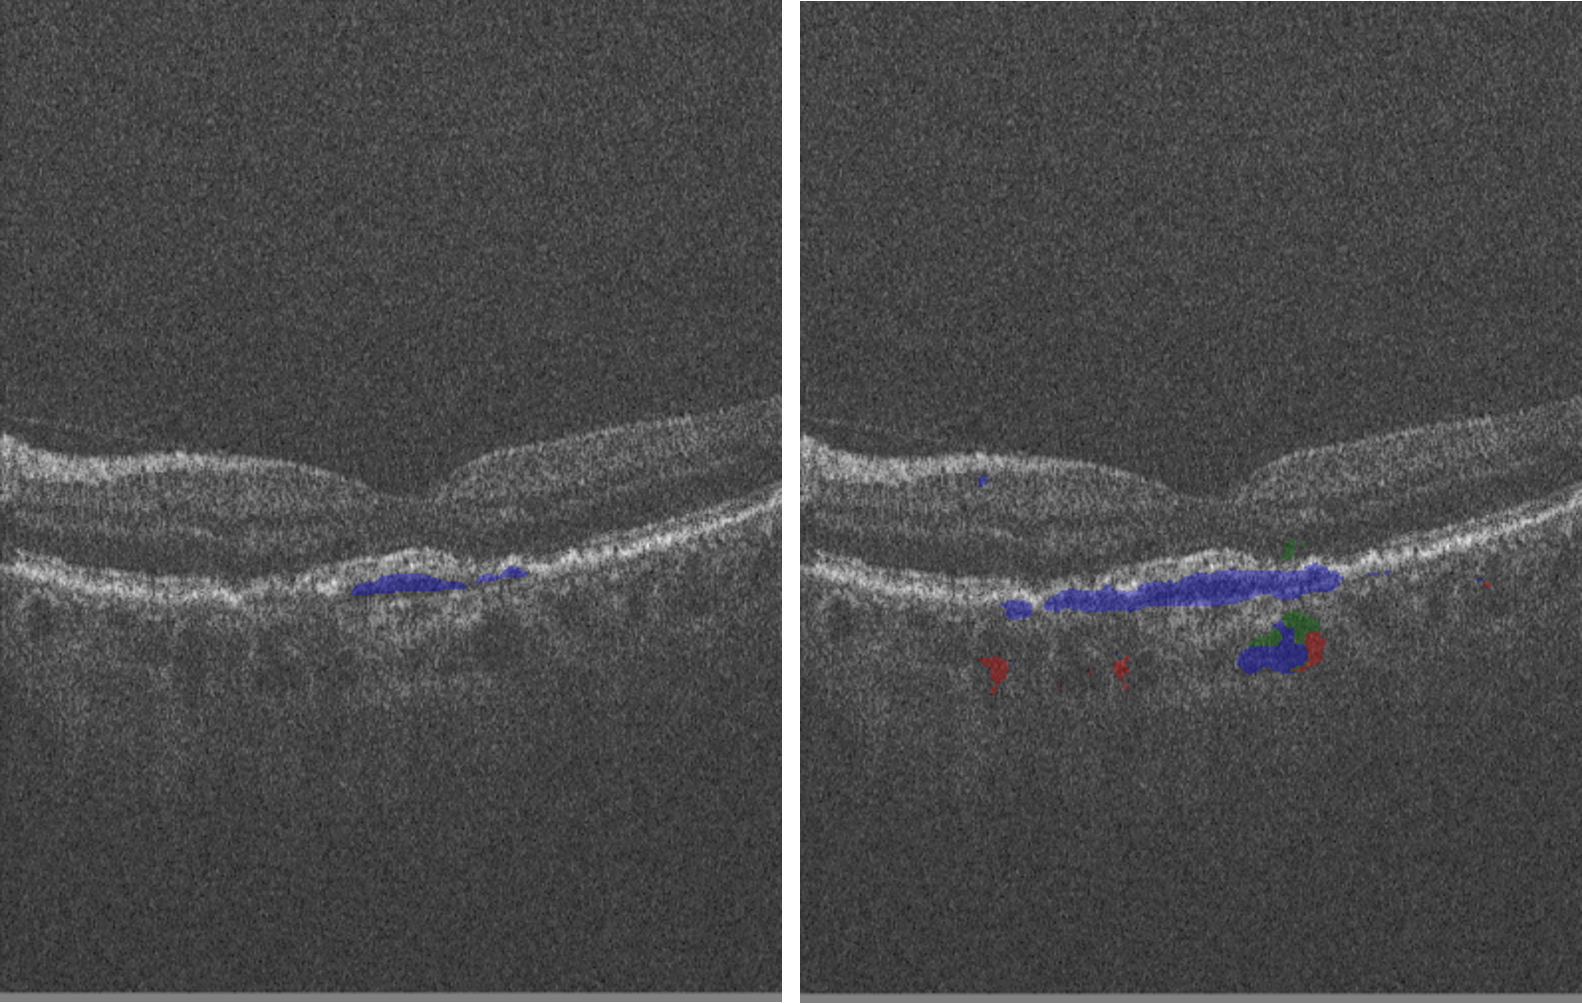
\includegraphics[width=0.6\linewidth]{figures/BigPatchSegmentationTopcon.png}
	\caption{Example of the segmentation done by the model trained in Run 12 (right) and its respective GT mask (left). It is noticeable that the model confuses the choroid with the retina, as segmentation of IRF and PED is performed in the choroid.}
	\label{fig:BigPatchesSegmentationTopcon}
\end{figure}

\subsubsection{Experiment 1.3 - Vertical Patch Extraction}
Experiment 1.3 contains all the runs that were performed using vertical patches extracted from resized B-scans as input of the multi-class segmentation U-Net. In the first two sets, shown in Table \ref{tab:Experiment1.3FourPatches}, the models were trained using four vertical patches, obtained as explained in the \ref{Methods} Materials and Methods chapter. In this table, the ``Set 4'' is composed of runs that were trained on 100 epochs, while the runs in ``Set 5'' were trained on up to 200 epochs with a 100 epoch patience.

\begin{table*}[!ht]
	\caption{Dice scores for every vendor and fluid for the runs done using four vertical patches extracted from each B-scan. In ``Set 4'', the models were trained in 100 epochs, while in ``Set 5'' the models were trained on up to 200 epochs with a 100 epoch patience. The transformations applied in these sets were the same: horizontal flipping and a maximum rotation of $10^{\circ}$.}
	\centering
	\resizebox{\textwidth}{!}{\begin{tabular}{|c|c|ccc|ccc|ccc|c|c|c|c|}
		\hline
		% Headers
		\multirow{2}{*}{\textbf{Runs}} & 
		\multirow{2}{*}{\textbf{VF}} & 
		\multicolumn{3}{c|}{\textbf{Cirrus}} & 
		\multicolumn{3}{c|}{\textbf{Spectralis}} & 
		\multicolumn{3}{c|}{\textbf{Topcon}} & 
		\multicolumn{1}{c|}{\multirow{2}{*}{\textbf{IRF}}} & 
		\multirow{2}{*}{\textbf{SRF}} & 
		\multirow{2}{*}{\textbf{PED}} & 
		\multirow{2}{*}{\textbf{Fluid}} \\ \cline{3-11} & &
		\multicolumn{1}{c}{\textbf{IRF}} & 
		\multicolumn{1}{c}{\textbf{SRF}} & 
		\textbf{\textbf{PED}} & 
		\multicolumn{1}{c}{\textbf{IRF}} & 
		\multicolumn{1}{c}{\textbf{SRF}} & 
		\textbf{PED} & 
		\textbf{IRF} & 
		\textbf{SRF} & 
		\textbf{PED} & 
		\multicolumn{1}{c|}{} & & & \\ 
			
		\hline
		
		\textbf{Run 13} & 2 & \multicolumn{1}{c|}{0.411} & \multicolumn{1}{c|}{0.665} & 0.498 & \multicolumn{1}{c|}{0.654} & \multicolumn{1}{c|}{0.735} & 0.611 & \multicolumn{1}{c|}{0.731} & \multicolumn{1}{c|}{0.743} & 0.519 & 0.563 & 0.704 & 0.526 & 0.581 \\

		\textbf{Run 14} & 3 & \multicolumn{1}{c|}{0.390} & \multicolumn{1}{c|}{0.520} & 0.217 & \multicolumn{1}{c|}{0.403} & \multicolumn{1}{c|}{0.564} & 0.429 & \multicolumn{1}{c|}{0.378} & \multicolumn{1}{c|}{0.754} & 0.477 & 0.388 & 0.614 & 0.350 & 0.386 \\
		
		\textbf{Run 15} & 4 & \multicolumn{1}{c|}{0.792} & \multicolumn{1}{c|}{\textbf{0.846}} & \textbf{0.883} & \multicolumn{1}{c|}{0.732} & \multicolumn{1}{c|}{\textbf{0.901}} & 0.733 & \multicolumn{1}{c|}{0.615} & \multicolumn{1}{c|}{0.758} & 0.656 & 0.707 & 0.815 & 0.765 & 0.652 \\
		
		\textbf{Run 16} & 0 & \multicolumn{1}{c|}{\textbf{0.810}} & \multicolumn{1}{c|}{0.834} & 0.715 & \multicolumn{1}{c|}{0.779} & \multicolumn{1}{c|}{0.857} & 0.753 & \multicolumn{1}{c|}{0.783} & \multicolumn{1}{c|}{\textbf{0.924}} & \textbf{0.882} & \textbf{0.795} & \textbf{0.871} & \textbf{0.783} & \textbf{0.709} \\
		
		\hline
		
		\textbf{Set 4} & - & \multicolumn{1}{c|}{\textbf{0.60}} & \multicolumn{1}{c|}{\textbf{0.72}} & 0.58 & \multicolumn{1}{c|}{0.64} & \multicolumn{1}{c|}{\textbf{0.76}} & 0.63 & \multicolumn{1}{c|}{0.63} & \multicolumn{1}{c|}{\textbf{0.79}} & 0.63 & 0.61 & \textbf{0.75} & 0.61 & 0.58 \\
		
		\hline
		\hline
		
		\textbf{Run 17} & 2 & \multicolumn{1}{c|}{0.522} & \multicolumn{1}{c|}{0.784} & 0.703 & \multicolumn{1}{c|}{\textbf{0.805}} & \multicolumn{1}{c|}{0.765} & \textbf{0.865} & \multicolumn{1}{c|}{\textbf{0.828}} & \multicolumn{1}{c|}{0.879} & 0.835 & 0.677 & 0.813 & 0.777 & 0.684 \\
	
		\textbf{Run 18} & 3 & \multicolumn{1}{c|}{0.509} & \multicolumn{1}{c|}{0.654} & 0.598 & \multicolumn{1}{c|}{0.590} & \multicolumn{1}{c|}{0.806} & 0.755 & \multicolumn{1}{c|}{0.777} & \multicolumn{1}{c|}{0.787} & 0.792 & 0.621 & 0.729 & 0.697 & 0.622 \\
					
		\textbf{Run 19} & 4 & \multicolumn{1}{c|}{0.377} & \multicolumn{1}{c|}{0.387} & 0.398 & \multicolumn{1}{c|}{0.478} & \multicolumn{1}{c|}{0.624} & 0.398 & \multicolumn{1}{c|}{0.483} & \multicolumn{1}{c|}{0.729} & 0.448 & 0.436 & 0.567 & 0.420 & 0.399 \\
		
		\textbf{Run 20} & 0 & \multicolumn{1}{c|}{0.753} & \multicolumn{1}{c|}{0.697} & 0.696 & \multicolumn{1}{c|}{0.779} & \multicolumn{1}{c|}{0.844} & 0.783 & \multicolumn{1}{c|}{0.691} & \multicolumn{1}{c|}{0.720} & 0.671 & 0.735 & 0.731 & 0.702 & 0.637 \\
		
		\hline
		
		\textbf{Set 5} & - & \multicolumn{1}{c|}{0.54} & \multicolumn{1}{c|}{0.63} & \textbf{0.60} & \multicolumn{1}{c|}{\textbf{0.66}} & \multicolumn{1}{c|}{0.76} & \textbf{0.70} & \multicolumn{1}{c|}{\textbf{0.69}} & \multicolumn{1}{c|}{0.78} & \textbf{0.69} & \textbf{0.62} & 0.71 & \textbf{0.65} & \textbf{0.59} \\
		
		\hline
			
	\end{tabular}}
	\label{tab:Experiment1.3FourPatches}
\end{table*}

The results of the sets shown in Table \ref{tab:Experiment1.3FourPatches} can be compared within each other and to the results obtained in the sets of previous experiments. 
\par
When comparing the results between sets, it is noticeable that the runs with the best scores are mostly located in the ``Set'' that trained less epochs. For, the model validated on fold 4 (Run 15) sees a significant decrease in performance when trained for 100 more epochs (Run 19). When looking at the models validation loss per epoch, the lowest value is attained commonly before the 100 epochs. Since the model that is saved in each run is the model that attains the lowest loss on validation data, this means that the models trained in 100 or 200 epochs should perform equally, as long as the lowest validation loss occurred prior to the 100 epoch mark.
\par
However, looking at Figure \ref{fig:TrainingValidationLosses}, where the training and validation loss curves for the Run 13 and Run 17 are shown, similar trends and behavior is seen in both models. This does not reflect to similar performances in the same validation data, as shown in Table \ref{tab:Experiment1.3FourPatches}. In fact, a substantial increment is seen in Run 17.
\par
To justify this behavior, it is important to remind that the training of a neural network has some randomness associated with it. One aspect that affects the model performance despite using the same data and architecture is the weight initialization. The random initialization of weights affects the trajectory of gradient descent, resulting in different convergences for different runs. Another factor that affects the model learning is the data that composes each batch. The images that form a batch are randomly fetch from the available input images. This create batches with different distributions of characteristics, affecting the model's view of the data. Data augmentation, which randomly selects images to apply the transformations as they are fetch, also influences the model performance. Lastly, there are other factors that have a much smaller impact such as the optimizer behavior and non-deterministic operations at the GPU level \parencite{Akesson2024, Altarabichi2024}. 
\par
In Appendix \ref{ap1:SegmentationUNetVariability}, Table \ref{tab:SegmentationUNetVariability} shows the results for multiple models that were trained on the same conditions, aiming to give an insight on how the randomness associated with the U-Net affects the models performances. Five models were validated on fold 2, while nine models were validated in fold 3. The results obtained corroborate the differences seen in Table \ref{tab:Experiment1.3FourPatches}, where models trained on the same conditions for more epochs can obtain significantly worse Dice scores in validation.

\begin{figure}[!ht]
	\centering
	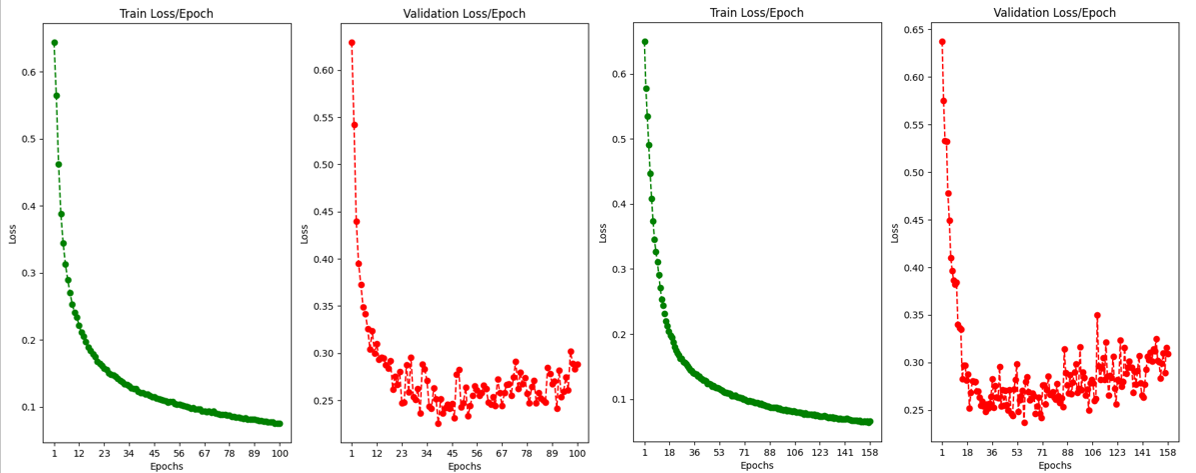
\includegraphics[width=1.0\linewidth]{figures/TrainingValidationLosses.png}
	\caption{Training and validation losses in Run 13 (left) and Run 17 (right). Despite reaching the validation loss minimum in a similar number of epochs and having comparable training and validation loss curves, the performance is really different in Table \ref{tab:Experiment1.3FourPatches}.}
	\label{fig:TrainingValidationLosses}
\end{figure}

Despite the differences in the results shown in Table \ref{tab:Experiment1.3FourPatches}, both sets attained better performances than the best results in the previous experiments. The improvements were significant, registering increases above 0.2 in some metrics when compared with the results in Experiment 1.3. Every vendor and every fluid seen a considerable increase of performance.
\par
This overall increment can be attributed to two changes: training on vertical patches and resizing the images. By training the models on vertical patches, the model can focus on the finer details within each region. This is important because the retinal fluid segmentation relies heavily on the retina's characteristics, a region that occupies a small portion of the image. Despite the input being smaller than in Experiment 1.2, the patches could still capture the transitions between the retina and the choroid or background. Since the input size is smaller, less storage it occupies in memory, therefore allowing an increase in the batch size, that translates to a faster and more stable convergence. Meanwhile, the image's resizing makes the inputs more homogeneous across different vendors. This results in the same structures being represented with consistent shapes and sizes across the B-scans from different vendors, resulting in a significantly simpler learning process.
\par
It was seen in Figure \ref{fig:BigPatchesSegmentationTopcon} that the model predicted fluid masks in the choroid region. In Figure \ref{fig:VerticalPatchesSegmentationTopcon}, it is seen that the models trained on vertical patches no longer predict fluid in the choroid region, despite inferring on the same B-scan. This means that, by feeding vertical patches to the model, it learns to not segment below the retina, in the choroid. This was not previously understood by the model when big patches were input, since these would frequently not capture both the retinal layer and the choroid in the same patch, restraining the model from learning the relative position of the choroid and its relationship with the fluid prediction.

\begin{figure}[!ht]
	\centering
	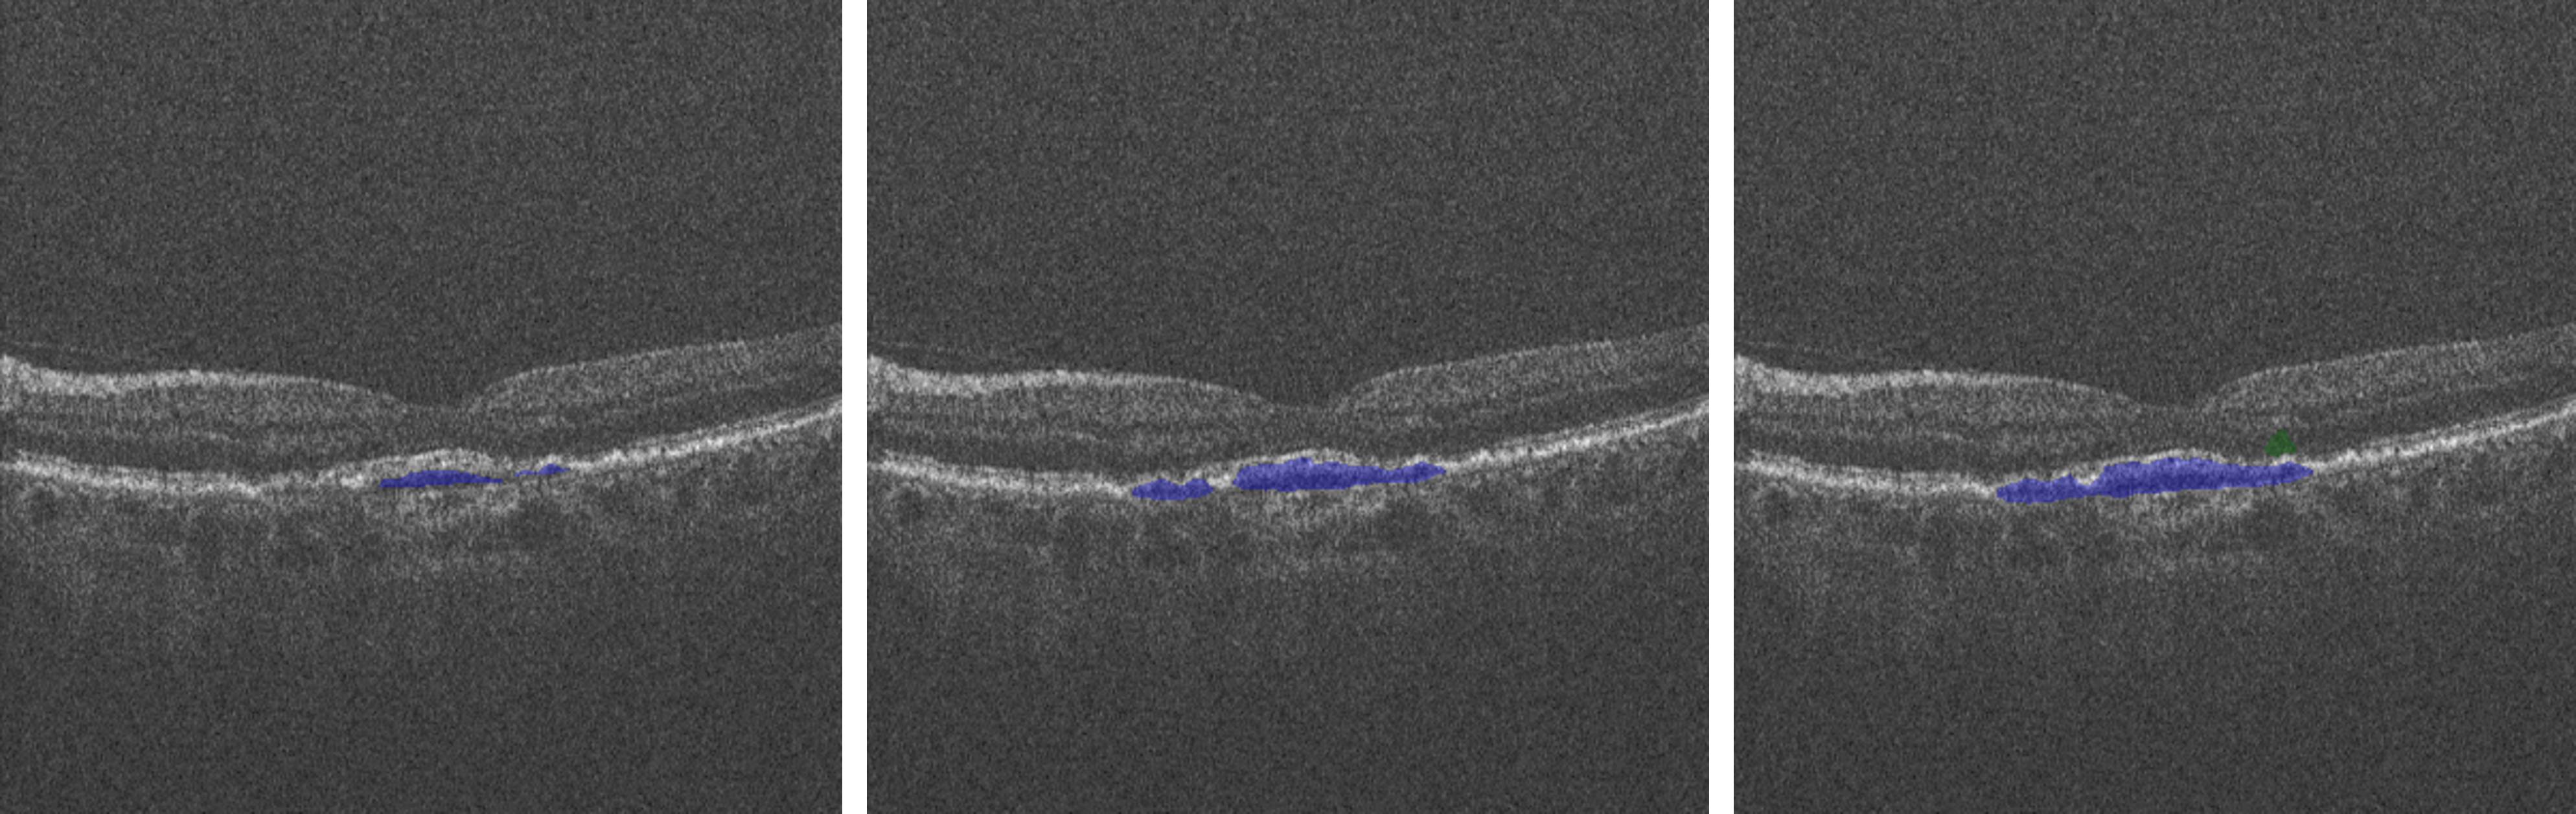
\includegraphics[width=1.0\linewidth]{figures/VerticalPatchesSegmentationTopcon.png}
	\caption{Predicted masks by the models trained on Run 16 (middle) and Run 20 (right) and their respective GT (left).}
	\label{fig:VerticalPatchesSegmentationTopcon}
\end{figure}

Afterwards, the use of seven and thirteen patches extracted from each B-scan was tested and the results are shown in Table \ref{tab:Experiment1.3SevenVsThirteenPatches}. Two models were trained for each number of patches extracted, one validated on fold 2 and another validated on fold 3. The models were trained on 200 maximum epochs, with a 25 epoch patience applied after the first 100 epochs.

\begin{table*}[!ht]
	\caption{Dice scores for every vendor and fluid for the runs done using seven (Runs 21 and 22) and thirteen (Runs 23 and 24) vertical patches extracted from each B-scan. Only two folds were used in order to understand the viability of using these numbers of patches, which are represented in the column ``P''. Runs 17 and 18 are shown here to make the comparison between the number of patches easier. The values shown in bold represent the best value for the models validated in the same fold.}
	\centering
	\resizebox{\textwidth}{!}{\begin{tabular}{|c|c|c|ccc|ccc|ccc|c|c|c|c|}
		\hline
		% Headers
		\multirow{2}{*}{\textbf{Runs}} & 
		\multirow{2}{*}{\textbf{VF}} & 
		\multirow{2}{*}{\textbf{P}} &
		\multicolumn{3}{c|}{\textbf{Cirrus}} & 
		\multicolumn{3}{c|}{\textbf{Spectralis}} & 
		\multicolumn{3}{c|}{\textbf{Topcon}} & 
		\multicolumn{1}{c|}{\multirow{2}{*}{\textbf{IRF}}} & 
		\multirow{2}{*}{\textbf{SRF}} & 
		\multirow{2}{*}{\textbf{PED}} & 
		\multirow{2}{*}{\textbf{Fluid}} \\ \cline{4-12} & & &
		\multicolumn{1}{c}{\textbf{IRF}} & 
		\multicolumn{1}{c}{\textbf{SRF}} & 
		\textbf{\textbf{PED}} & 
		\multicolumn{1}{c}{\textbf{IRF}} & 
		\multicolumn{1}{c}{\textbf{SRF}} & 
		\textbf{PED} & 
		\textbf{IRF} & 
		\textbf{SRF} & 
		\textbf{PED} & 
		\multicolumn{1}{c|}{} & & & \\ 
		
		\hline
			
		\textbf{Run 17} & 2 & 4 & \multicolumn{1}{c|}{0.522} & \multicolumn{1}{c|}{0.784} & \textbf{0.703} & \multicolumn{1}{c|}{\textbf{0.805}} & \multicolumn{1}{c|}{0.765} & \textbf{0.865} & \multicolumn{1}{c|}{0.828} & \multicolumn{1}{c|}{0.879} & 0.835 & 0.677 & 0.813 & \textbf{0.777} & 0.684 \\
		
		\textbf{Run 21} & 2 & 7 & \multicolumn{1}{c|}{\textbf{0.556}} & \multicolumn{1}{c|}{\textbf{0.837}} & 0.672 & \multicolumn{1}{c|}{0.761} & \multicolumn{1}{c|}{\textbf{0.853}} & 0.848 & \multicolumn{1}{c|}{\textbf{0.829}} & \multicolumn{1}{c|}{0.908} & \textbf{0.858} & \textbf{0.685} & \textbf{0.864} & 0.767 & \textbf{0.681} \\
		
		\textbf{Run 23} & 2 & 13 & \multicolumn{1}{c|}{0.500} & \multicolumn{1}{c|}{0.762} & 0.635 & \multicolumn{1}{c|}{0.672} & \multicolumn{1}{c|}{0.790} & 0.773 & \multicolumn{1}{c|}{0.819} & \multicolumn{1}{c|}{\textbf{0.936}} & 0.805 & 0.639 & 0.826 & 0.718 & 0.637 \\
		
		\hline
		\hline
		
		\textbf{Run 18} & 3 & 4 & \multicolumn{1}{c|}{0.509} & \multicolumn{1}{c|}{0.654} & 0.598 & \multicolumn{1}{c|}{0.590} & \multicolumn{1}{c|}{0.806} & \textbf{0.755} & \multicolumn{1}{c|}{\textbf{0.777}} & \multicolumn{1}{c|}{\textbf{0.787}} & \textbf{0.792} & 0.621 & 0.729 & 0.697 & 0.622 \\
		
		\textbf{Run 22} & 3 & 7 & \multicolumn{1}{c|}{\textbf{0.734}} & \multicolumn{1}{c|}{\textbf{0.855}} & 0.836 & \multicolumn{1}{c|}{\textbf{0.636}} & \multicolumn{1}{c|}{\textbf{0.846}} & 0.689 & \multicolumn{1}{c|}{0.686} & \multicolumn{1}{c|}{0.781} & 0.731 & \textbf{0.700} & \textbf{0.822} & \textbf{0.771} & \textbf{0.672} \\
		
		\textbf{Run 24} & 3 & 13 & \multicolumn{1}{c|}{0.612} & \multicolumn{1}{c|}{0.648} & \textbf{0.882} & \multicolumn{1}{c|}{0.455} & \multicolumn{1}{c|}{0.636} & 0.548 & \multicolumn{1}{c|}{0.499} & \multicolumn{1}{c|}{0.593} & 0.668 & 0.542 & 0.622 & 0.745 & 0.536 \\
		
		\hline
			
	\end{tabular}}
	\label{tab:Experiment1.3SevenVsThirteenPatches}
\end{table*}

Training the models on more patches per B-scan, significantly increases the quantity of data that is seen by the model during an epoch. Therefore, each epoch takes much longer to complete, requiring more computation power, leading to often bottlenecks. However, since the model sees many more patches per epoch, the model reaches the validation loss minimum much earlier than in the models trained with four patches. 
\par
In Figure \ref{fig:ValidationLossesFourSevenThirteenPatches}, it is possible to see a comparison between the training and validation losses of the models validated on fold 2, using four, seven, and thirteen vertical patches per B-scan. Despite following the same trends, the model learns significantly faster as the number of patches increases, resulting in a faster progression of the validation loss. As a result the models starts to overfit much earlier and aggressively with larger number of patches, which is signaled by the increase in validation loss after reaching low values.

\begin{figure}[!ht]
	\centering
	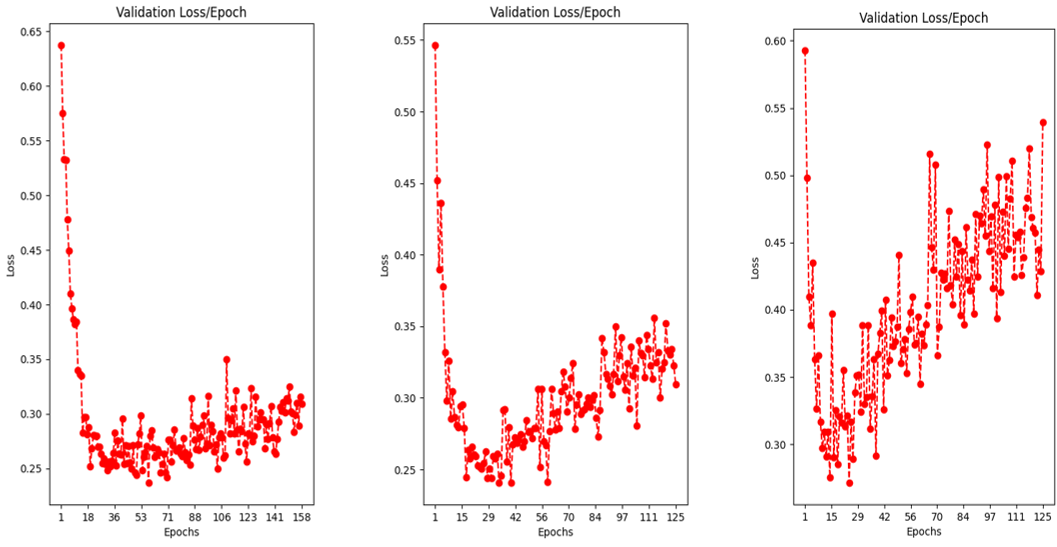
\includegraphics[width=1.0\linewidth]{figures/ValidationLossesFourSevenThirteenPatches.png}
	\caption{Training and validation losses for models validated on fold 2. The curve on the left are from the model trained on Run 17 with four patches, while the middle curves are from the model trained on Run 21, with seven patches. The curves on the right are from the model trained on Run 23, with thirteen patches.}
	\label{fig:ValidationLossesFourSevenThirteenPatches}
\end{figure}

When comparing the models' performances, by looking at Table \ref{tab:Experiment1.3FourPatches}, the models trained on thirteen patches are outperformed by those trained in fewer patches. These results suggest that the faster progression in validation loss for the model trained with thirteen patches inhibits its ability to converge to a solution as optimal as those achieved by models trained more slowly with fewer patches.
\par
The performance differences between the models trained with four and seven patches are smaller than the difference between either of those models and the model trained with thirteen patches. However, the model trained with seven patches consistently outperforms the one trained with four in most metrics. In the few cases the model trained with four patches performs better, the other model still achieves comparable results. The reverse is not true: when the model trained with seven patches outperforms the model trained with four patches, the performance gap is significantly larger. For these reasons, the model trained with seven patches was considered superior.
\par
Nevertheless, both models still make wrongful predictions, which do not respect the anatomic context of the image. For example, in Figure \ref{fig:CirrusSegmentationErrors}, the IRF fluid is predicted below the PED, which is not anatomically possible and there are no examples in the dataset that exhibit this relationship.
\par
While this unexpected behavior could be attributed to the B-scan differing from the examples seen in training, the subsequent runs aimed to investigate whether this was caused by the rotation transformation. It was hypothesized that random rotations could alter the vertical order of fluid regions, potentially leading the model to learn incorrect patterns. Additionally, the padding that is performed to fill the rotated areas, as illustrated in Figure \ref{fig:TransformationsInVerticalPatches}, could also influence the model's performance.

\begin{figure}[!ht]
	\centering
	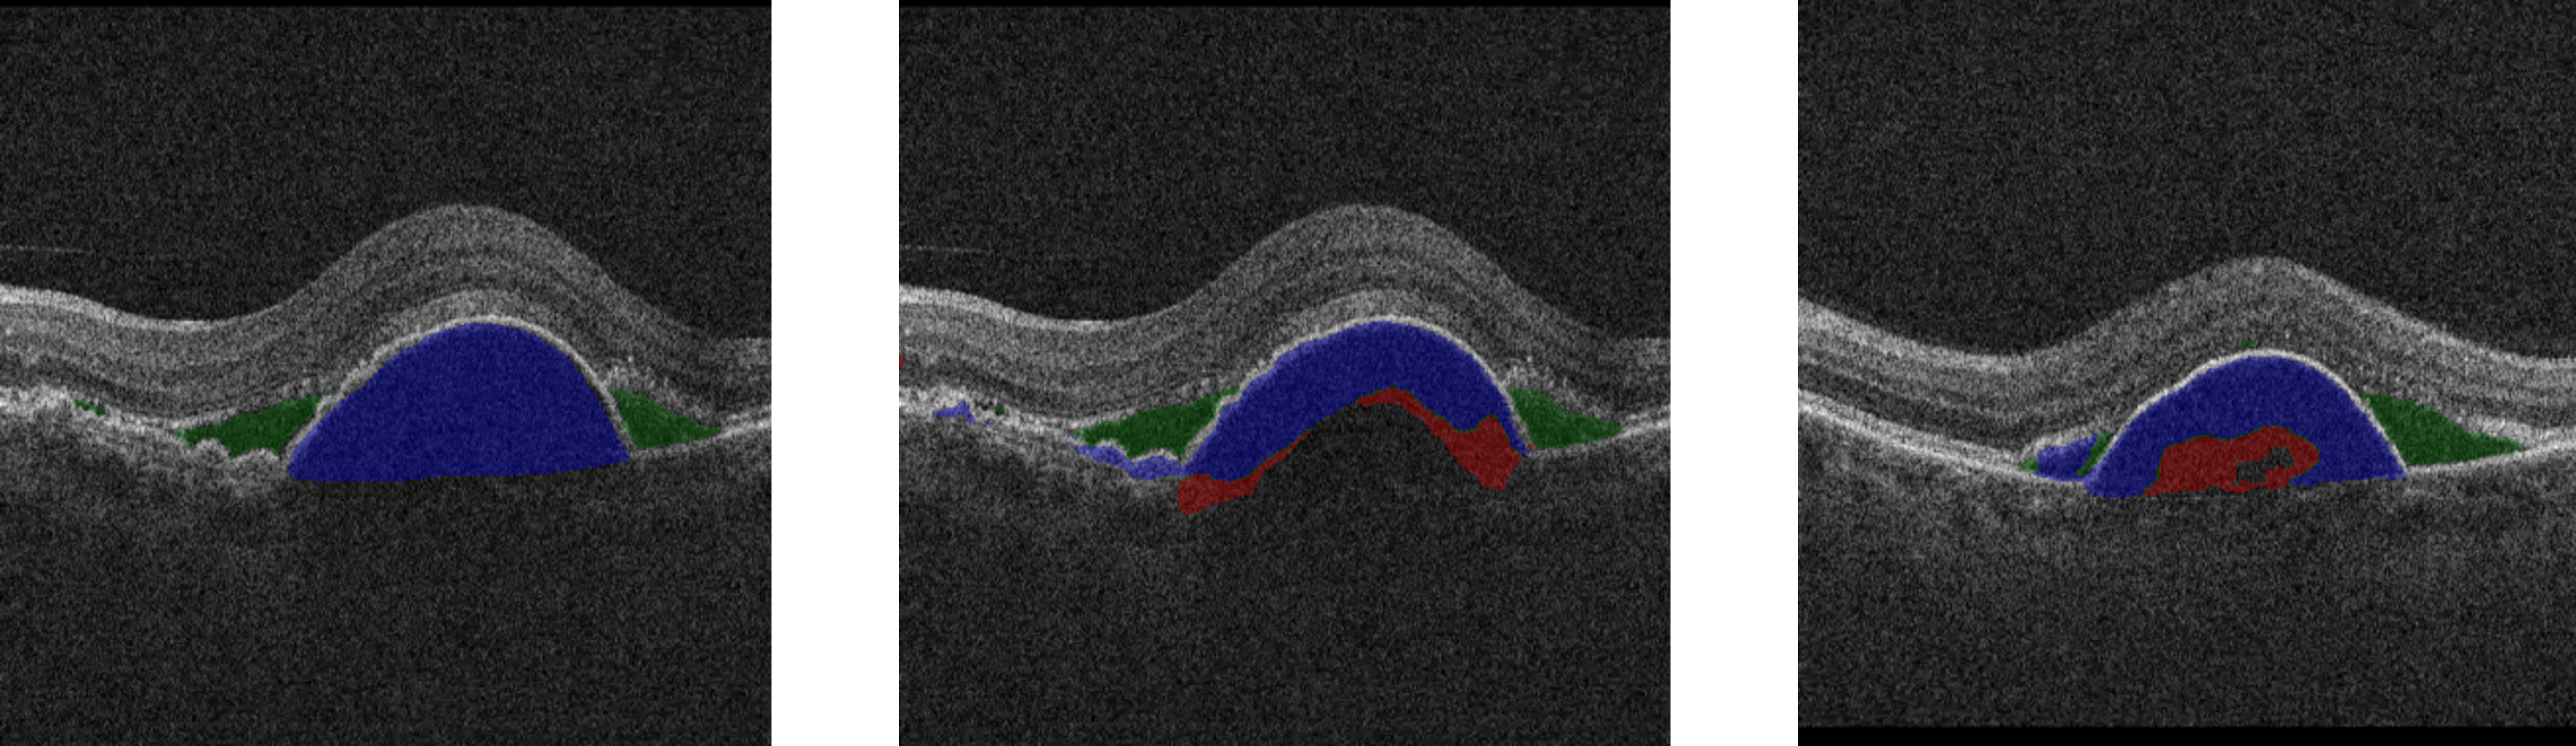
\includegraphics[width=1.0\linewidth]{figures/CirrusSegmentationErrors.png}
	\caption{Segmentation errors in Cirrus B-scans. The GT fluid masks, seen on the left, show a large region of PED fluid. Meanwhile, the predictions made by the models trained in Run 21 and 23, which respectively correspond to the B-scans in the middle and right, classify the center of this region as IRF.}
	\label{fig:CirrusSegmentationErrors}
\end{figure}

\begin{figure}[!ht]
	\centering
	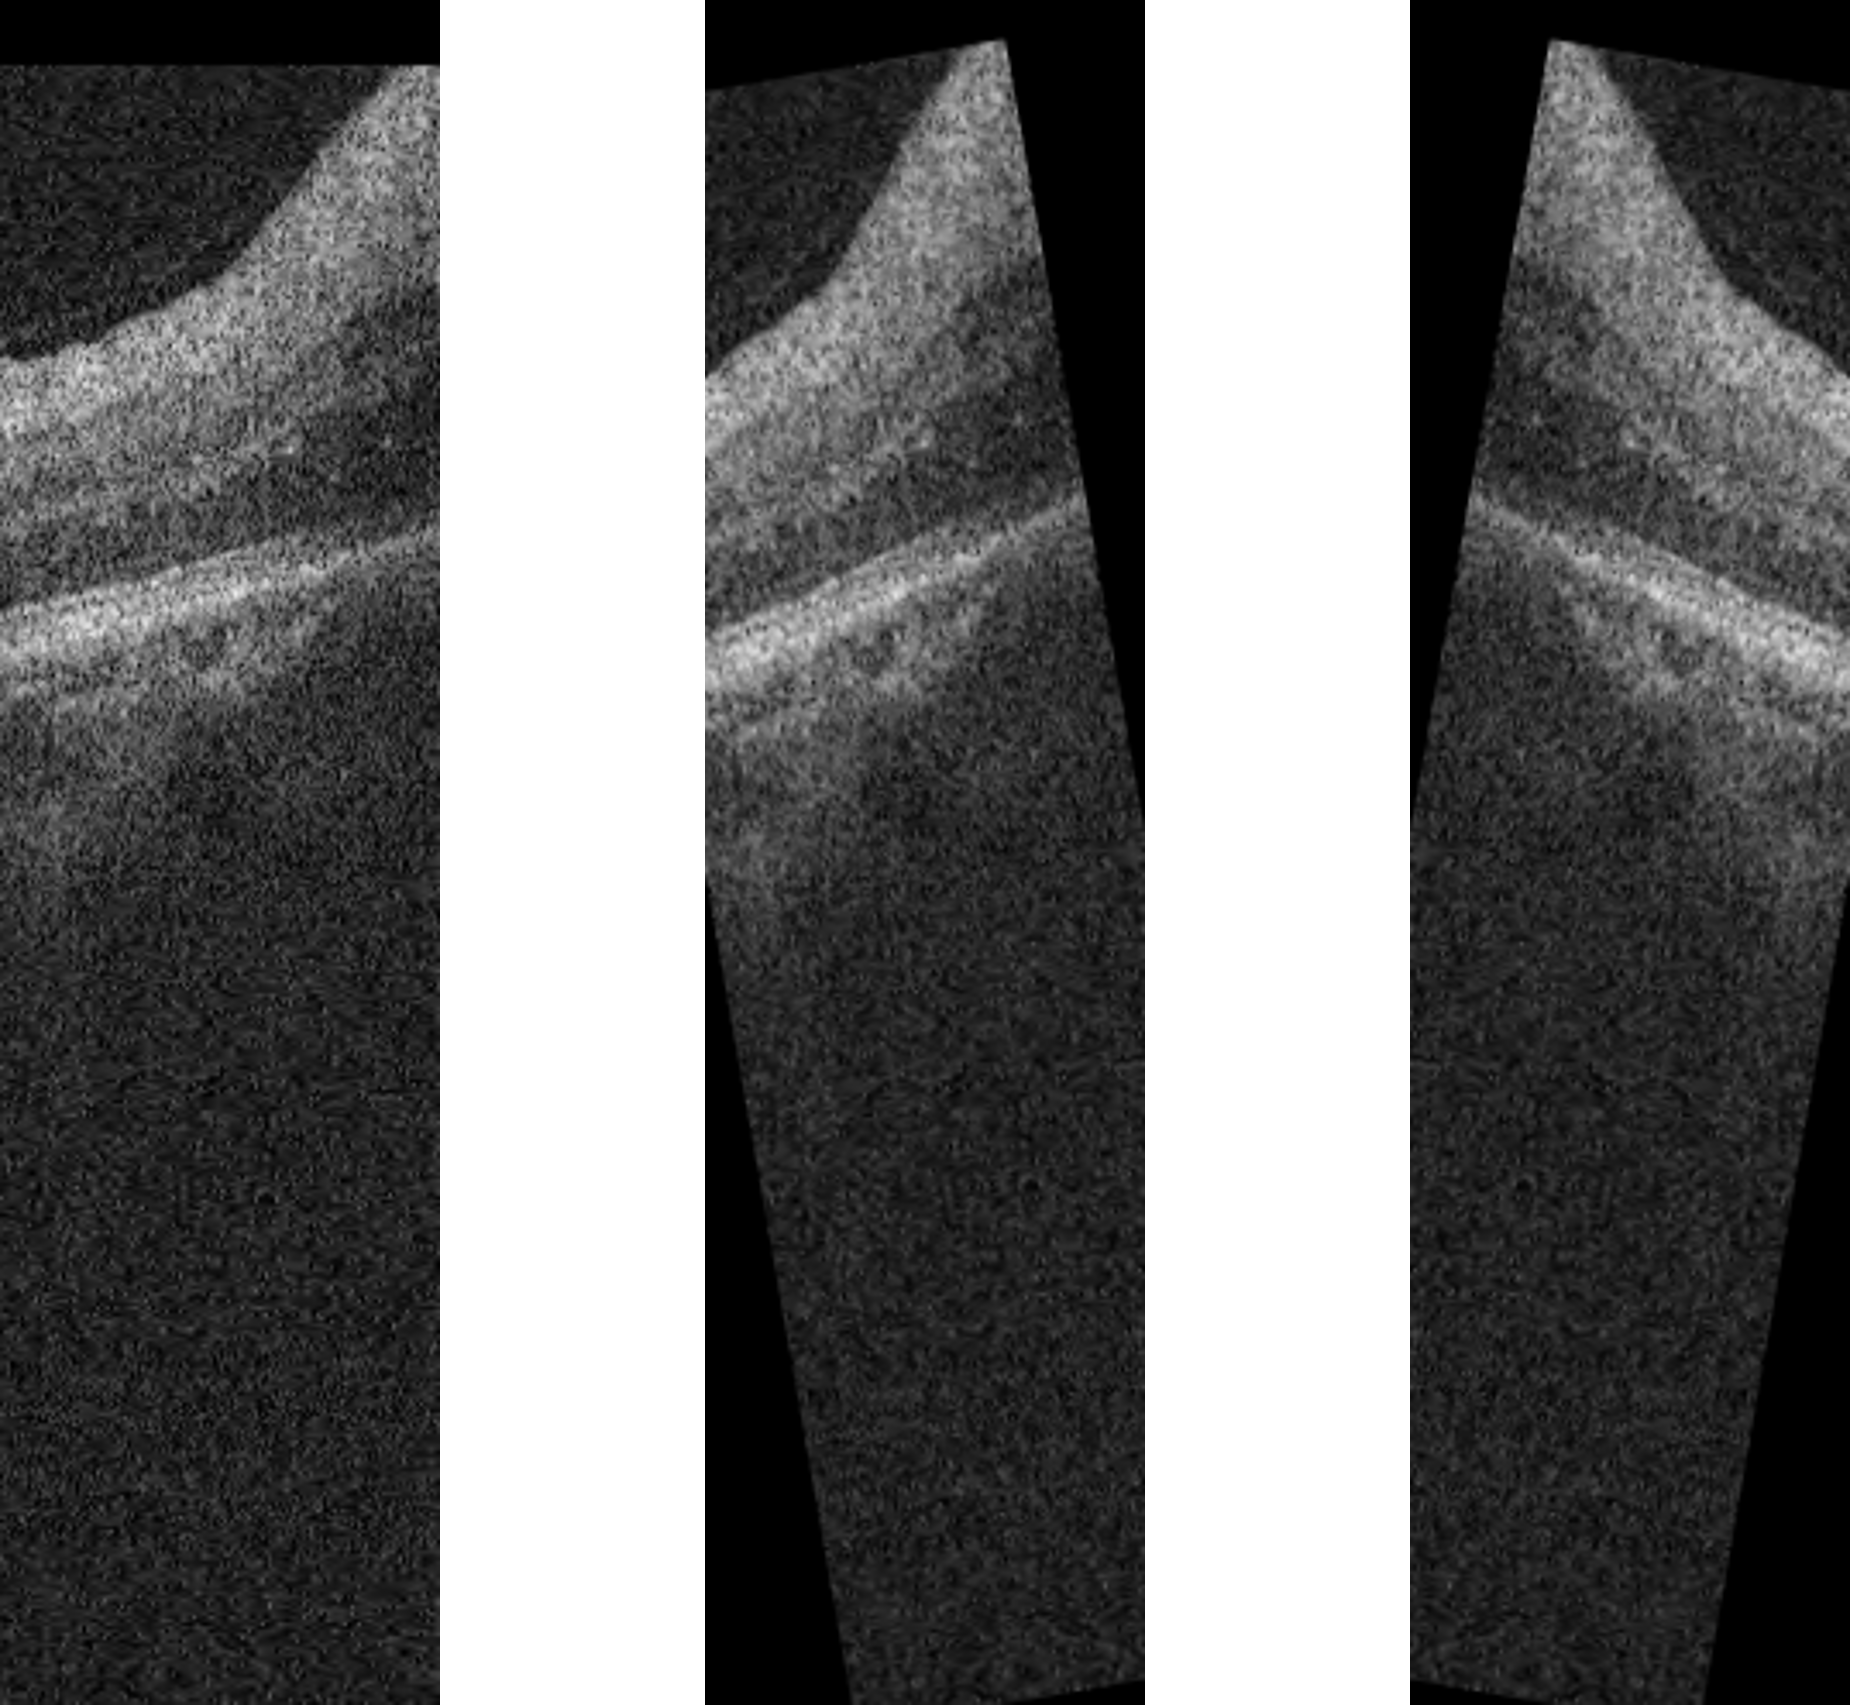
\includegraphics[width=0.5\linewidth]{figures/TransformationsInVerticalPatches.png}
	\caption{Transformations applied to a vertical patch of a Cirrus B-scan. The original vertical patch (left) can be rotated a maximum of $10^{\circ}$, a transformation that is shown in the middle image. The image on the right represents the combination of a $10^{\circ}$ rotation and an horizontal flip. It is seen that the rotation transform pads a significant portion of the image, reducing the information in the input.}
	\label{fig:TransformationsInVerticalPatches}
\end{figure}

Table \ref{tab:Experiment1.3SevenPatchesNoRotation} shows the results obtained in the runs performed using only horizontal flipping as transformation, without performing rotations. In these runs, seven input patches were extracted from each B-scan. Due to the faster progression of the models trained using seven vertical patches per B-scan, the model was trained on a minimum of 25 epochs with a 25 epoch patience after. Since the validation minimum is usually attained early in the models trained with more patches, as seen in Figure \ref{fig:ValidationLossesFourSevenThirteenPatches}, by setting such early stopping, the training duration would be shorter while maintaining the same performance.

\begin{table*}[!ht]
	\caption{Dice scores for every vendor and fluid using seven vertical patches. The only transformation performed in these runs was horizontal flipping, without rotation. Runs 21 and 22 are also shown, promoting an easier comparison.}
	\centering
	\resizebox{\textwidth}{!}{\begin{tabular}{|c|c|ccc|ccc|ccc|c|c|c|c|}
			\hline
			% Headers
			\multirow{2}{*}{\textbf{Runs}} & 
			\multirow{2}{*}{\textbf{VF}} & 
			\multicolumn{3}{c|}{\textbf{Cirrus}} & 
			\multicolumn{3}{c|}{\textbf{Spectralis}} & 
			\multicolumn{3}{c|}{\textbf{Topcon}} & 
			\multicolumn{1}{c|}{\multirow{2}{*}{\textbf{IRF}}} & 
			\multirow{2}{*}{\textbf{SRF}} & 
			\multirow{2}{*}{\textbf{PED}} & 
			\multirow{2}{*}{\textbf{Fluid}} \\ \cline{3-11} & &
			\multicolumn{1}{c}{\textbf{IRF}} & 
			\multicolumn{1}{c}{\textbf{SRF}} & 
			\textbf{\textbf{PED}} & 
			\multicolumn{1}{c}{\textbf{IRF}} & 
			\multicolumn{1}{c}{\textbf{SRF}} & 
			\textbf{PED} & 
			\textbf{IRF} & 
			\textbf{SRF} & 
			\textbf{PED} & 
			\multicolumn{1}{c|}{} & & & \\ 
			
			\hline
			
			\textbf{Run 25} & 2 & \multicolumn{1}{c|}{0.406} & \multicolumn{1}{c|}{0.789} & 0.656 & \multicolumn{1}{c|}{0.595} & \multicolumn{1}{c|}{\textbf{0.805}} & \textbf{0.786} & \multicolumn{1}{c|}{0.762} & \multicolumn{1}{c|}{0.841} & 0.797 & 0.560 & 0.809 & 0.727 & 0.620 \\

			
			\textbf{Run 26} & 3 & \multicolumn{1}{c|}{0.589} & \multicolumn{1}{c|}{0.775} & 0.553 & \multicolumn{1}{c|}{0.586} & \multicolumn{1}{c|}{0.803} & 0.766 & \multicolumn{1}{c|}{0.769} & \multicolumn{1}{c|}{\textbf{0.827}} & 0.755 & 0.654 & 0.799 & 0.664 & 0.617 \\
			
			
			\textbf{Run 27} & 4 & \multicolumn{1}{c|}{\textbf{0.797}} & \multicolumn{1}{c|}{\textbf{0.845}} & \textbf{0.827} & \multicolumn{1}{c|}{\textbf{0.734}} & \multicolumn{1}{c|}{0.782} & 0.659 & \multicolumn{1}{c|}{0.533} & \multicolumn{1}{c|}{0.756} & 0.553 & 0.674 & 0.798 & 0.686 & 0.626 \\
			
			
			\textbf{Run 28} & 0 & \multicolumn{1}{c|}{0.677} & \multicolumn{1}{c|}{0.842} & 0.699 & \multicolumn{1}{c|}{0.681} & \multicolumn{1}{c|}{0.799} & 0.732 & \multicolumn{1}{c|}{\textbf{0.791}} & \multicolumn{1}{c|}{0.846} & \textbf{0.854} & \textbf{0.719} & \textbf{0.836} & \textbf{0.762} & \textbf{0.665} \\
			
			
			\hline
			
			\textbf{Set 6} & - & \multicolumn{1}{c|}{0.62} & \multicolumn{1}{c|}{0.81} & 0.68 & \multicolumn{1}{c|}{0.65} & \multicolumn{1}{c|}{0.80} & 0.74 & \multicolumn{1}{c|}{0.71} & \multicolumn{1}{c|}{0.82} & 0.74 & 0.65 & 0.81 & 0.71 & 0.63 \\
			
			\hline
			\hline
			
			\textbf{Run 21} & 2 & \multicolumn{1}{c|}{0.556} & \multicolumn{1}{c|}{0.837} & 0.672 & \multicolumn{1}{c|}{0.761} & \multicolumn{1}{c|}{0.853} & 0.848 & \multicolumn{1}{c|}{0.829} & \multicolumn{1}{c|}{0.908} & 0.858 & 0.685 & 0.864 & 0.767 & 0.681 \\
			
			\textbf{Run 22} & 3 & \multicolumn{1}{c|}{0.734} & \multicolumn{1}{c|}{0.855} & 0.836 & \multicolumn{1}{c|}{0.636} & \multicolumn{1}{c|}{0.846} & 0.689 & \multicolumn{1}{c|}{0.686} & \multicolumn{1}{c|}{0.781} & 0.731 & 0.700 & 0.822 & 0.771 & 0.672 \\
			
			\hline
			
	\end{tabular}}
	\label{tab:Experiment1.3SevenPatchesNoRotation}
\end{table*}

Removing the rotation from the transformations applied to the input data, significantly worsen the models performances. In Table \ref{tab:Experiment1.3SevenPatchesNoRotation}, when comparing Run 21 to Run 25, which were validated on the same fold, the model trained in Run 21, with rotation, outperformed the model trained in Run 25 in every single metric. Following the same trend, the model trained in Run 26 only outperformed the model trained in Run 22 in four metrics: Spectralis PED and all the fluids in Topcon.
\par
The differences in performance here exposed highlight the importance of applying transformations to the inputs, despite the mentioned loss of information associated with it. The introduction of variability to the input data significantly improved the model's generalization, preventing the model from overfitting so early on the training stage. In OCT, the rotation is particularly important since different images exhibit different orientations of the retinal layer. By introducing rotation to the inputs, the model becomes more robust to varied input data and less specific to the orientations seen in training. This transformation particularly enhances the performance of the models trained in B-scans where the retinal layer appears horizontal. In Figure \ref{fig:DifferentRetinaOrientation}, two B-scans that illustrate the variability of the retina orientation are shown.
\par
Nevertheless, the lack of rotation in the training dataset mitigated the poor segmentation shown in Figure \ref{fig:CirrusSegmentationErrors}. As exhibited in Figure \ref{fig:SegmentationErrorsNoRotation}, the model that was trained without rotation does not predict as much IRF in the PED region as those trained with rotation, as shown in Figure \ref{fig:CirrusSegmentationErrors}. However, the model that was trained without rotation also predicted IRF in a region that none of the other models did, exemplifying why this model performed worse than those.

\begin{figure}[!ht]
	\centering
	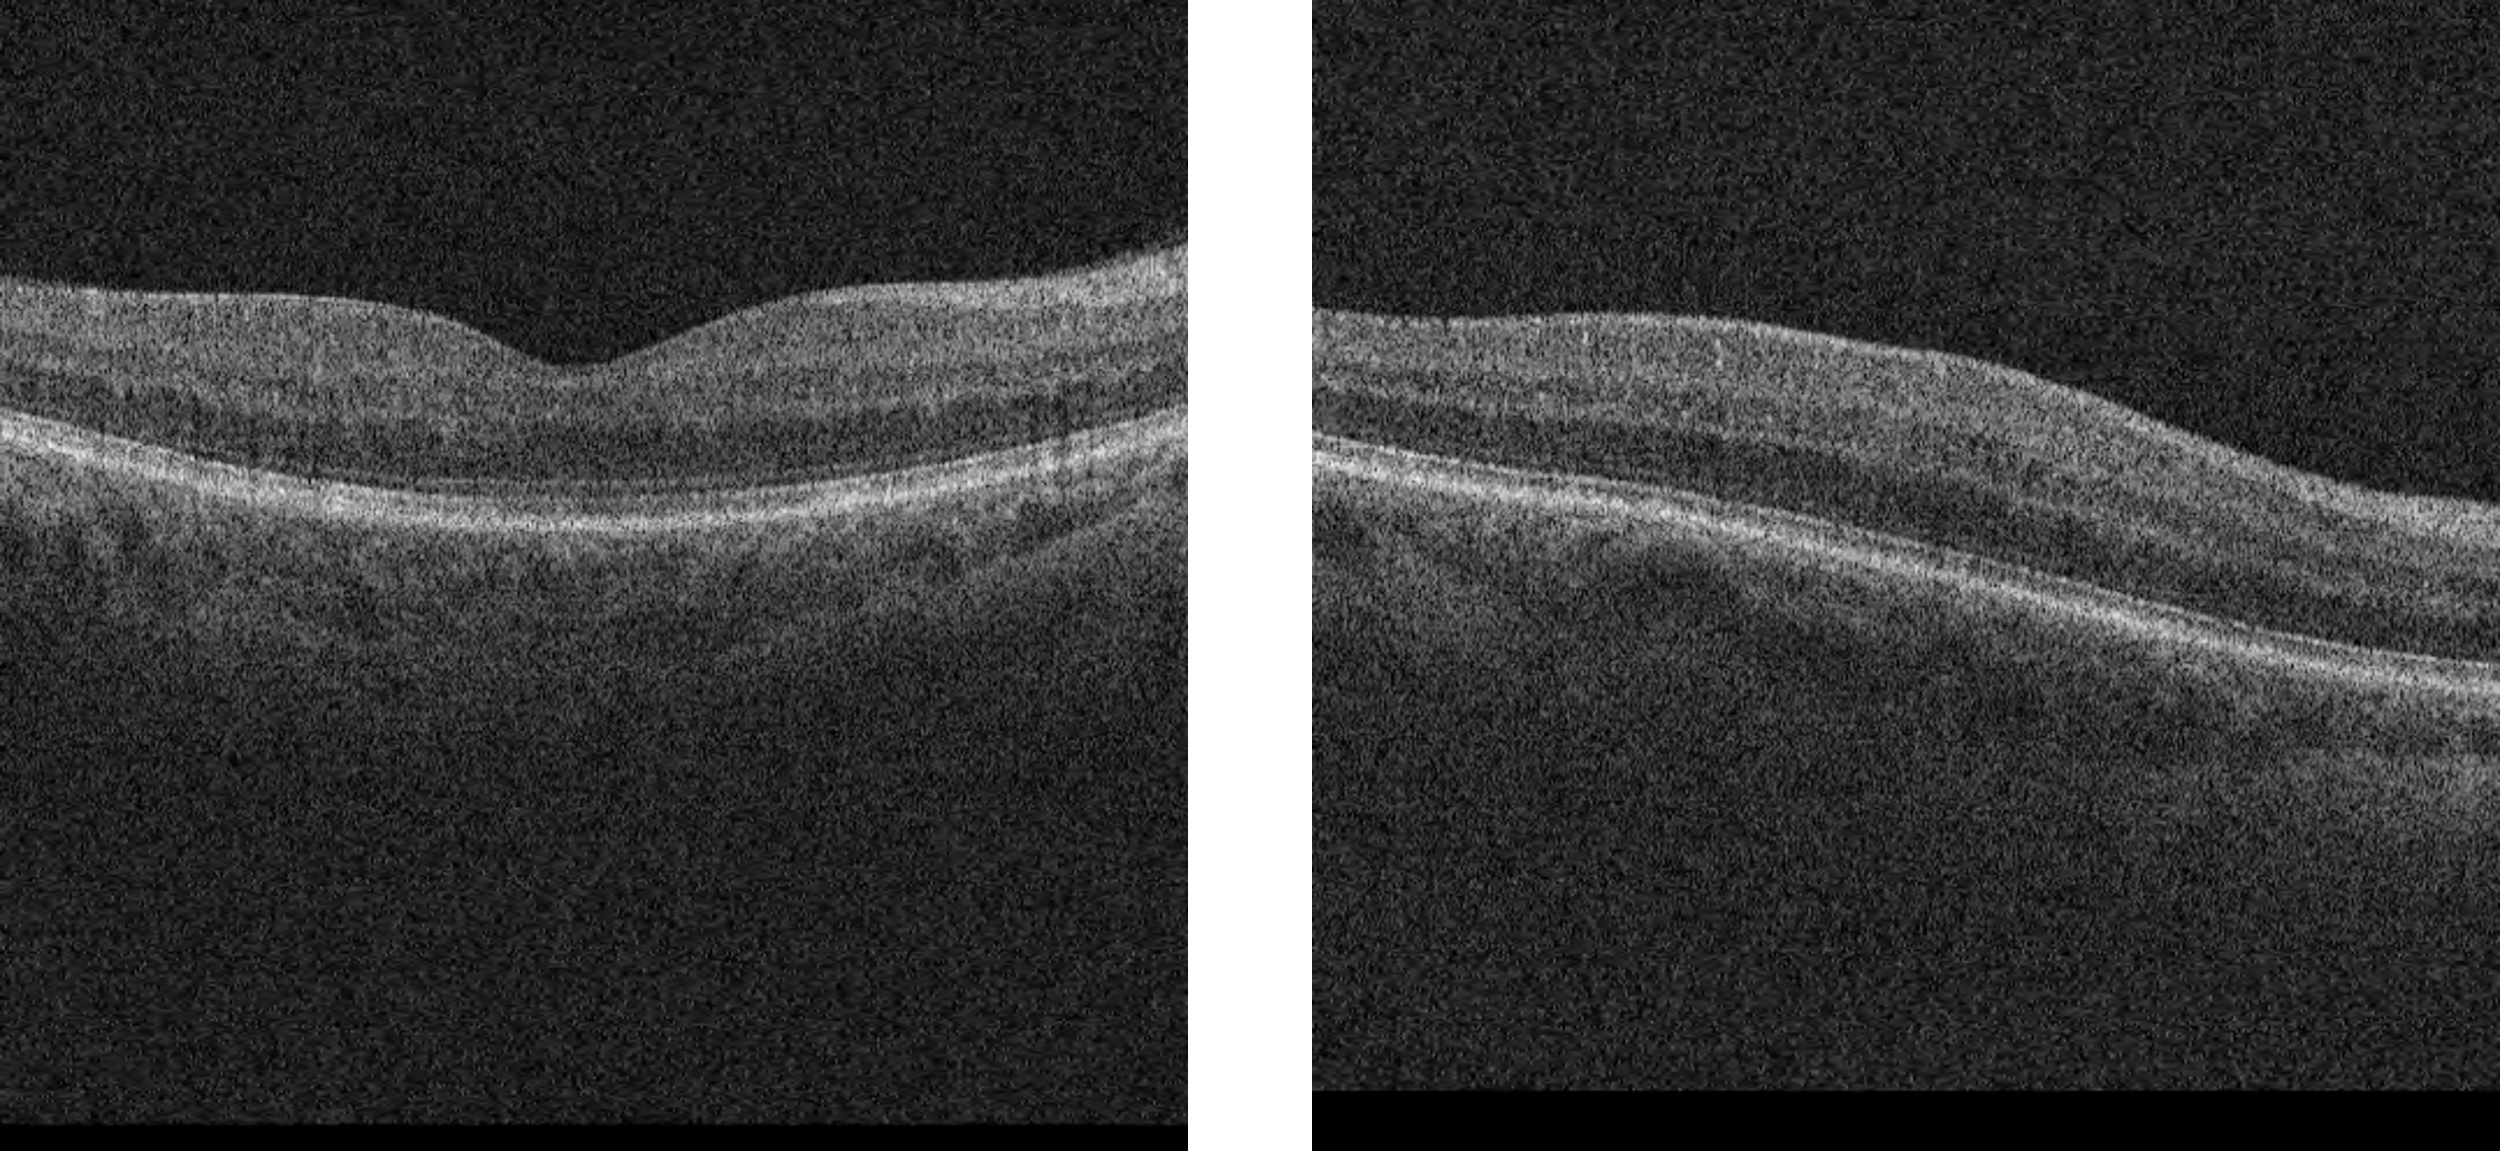
\includegraphics[width=0.7\linewidth]{figures/DifferentRetinaOrientation.png}
	\caption{Example of two B-scans in which the retina is oriented differently. The retina present in the right image is significantly more inclined. Both B-scans were obtained using a Cirrus device and do not present fluid.}
	\label{fig:DifferentRetinaOrientation}
\end{figure}

\begin{figure}[!ht]
	\centering
	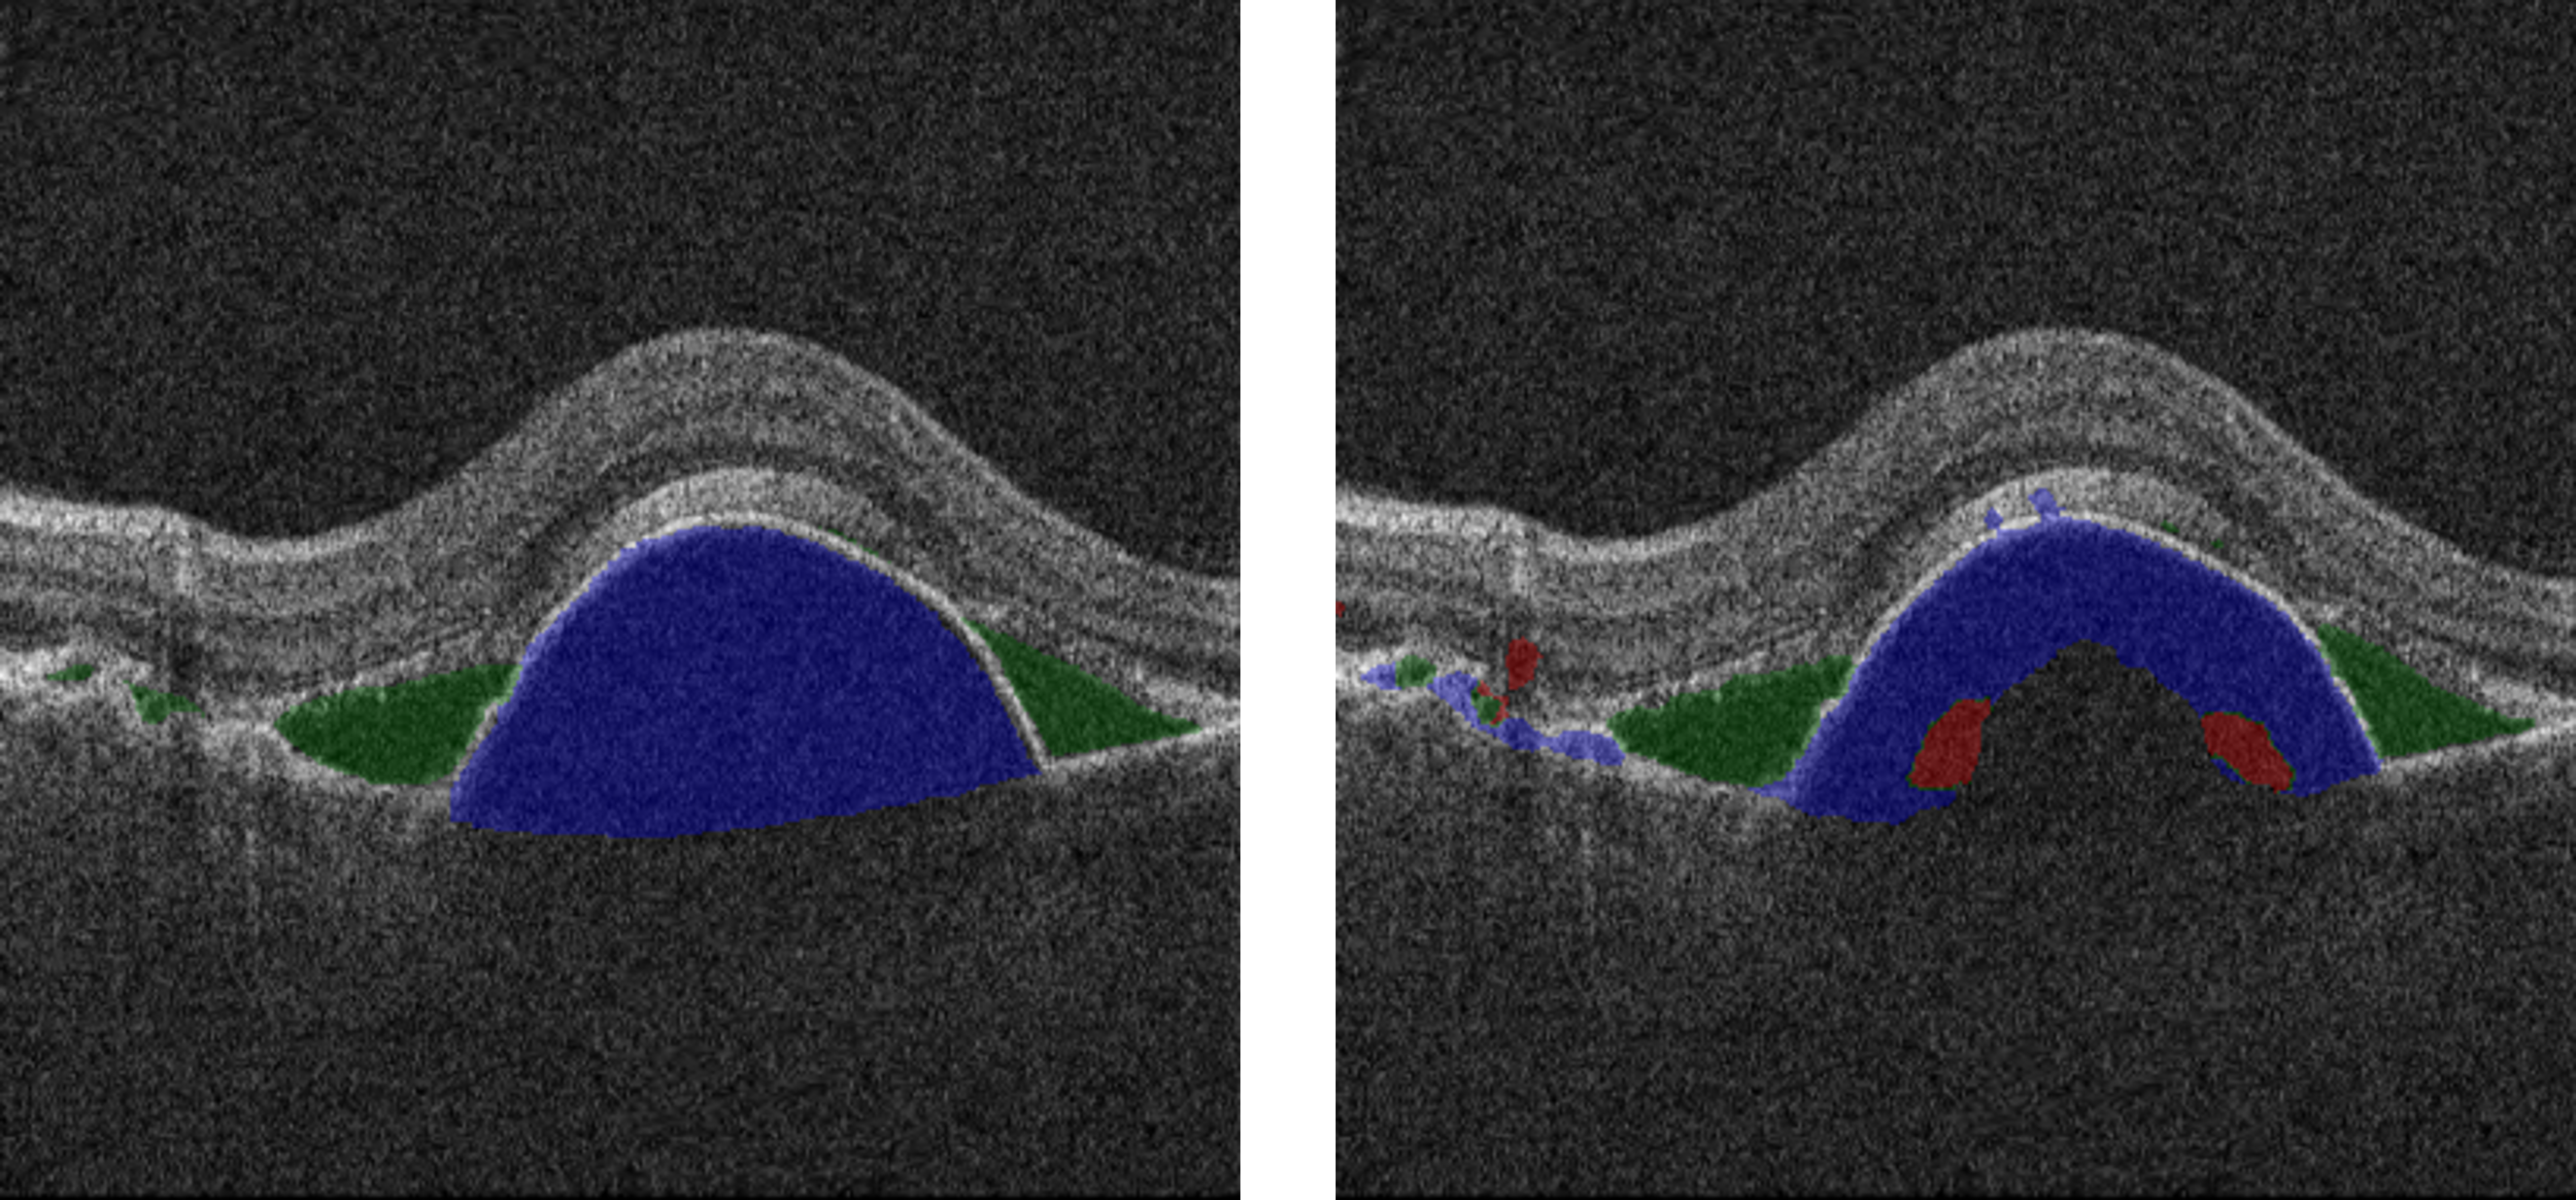
\includegraphics[width=0.7\linewidth]{figures/SegmentationErrorsNoRotation.png}
	\caption{Segmentation errors in Cirrus B-scans when trained without random rotations, in the same B-scan as in Figure \ref{fig:CirrusSegmentationErrors}. In the left, the GT masks are shown, while in the right the predicted masks are exhibited.}
	\label{fig:SegmentationErrorsNoRotation}
\end{figure}

In order to find an equilibrium between the robustness that training a model with rotated patches brings and the respect for the vertical order and relationships of the fluids, new runs were performed with a maximum $5^{\circ}$ rotation combined with the horizontal flipping. This rotation does not remove as much information from the patches as a $10^{\circ}$ rotation. The results obtained in these runs are shown in Table \ref{tab:Experiment1.3SevenPatches5DegreeRotation}.

\begin{table*}[!ht]
	\caption{Dice scores for every vendor and fluid using seven vertical patches. In these runs, horizontal flipping and $5^{\circ}$ rotation were used, instead of the usual $10^{\circ}$. The results obtained in Runs 21 and 22 are also shown, enabling a smoother comparison.}
	\centering
	\resizebox{\textwidth}{!}{\begin{tabular}{|c|c|ccc|ccc|ccc|c|c|c|c|}
		\hline
		% Headers
		\multirow{2}{*}{\textbf{Runs}} & 
		\multirow{2}{*}{\textbf{VF}} & 
		\multicolumn{3}{c|}{\textbf{Cirrus}} & 
		\multicolumn{3}{c|}{\textbf{Spectralis}} & 
		\multicolumn{3}{c|}{\textbf{Topcon}} & 
		\multicolumn{1}{c|}{\multirow{2}{*}{\textbf{IRF}}} & 
		\multirow{2}{*}{\textbf{SRF}} & 
		\multirow{2}{*}{\textbf{PED}} & 
		\multirow{2}{*}{\textbf{Fluid}} \\ \cline{3-11} & &
		\multicolumn{1}{c}{\textbf{IRF}} & 
		\multicolumn{1}{c}{\textbf{SRF}} & 
		\textbf{\textbf{PED}} & 
		\multicolumn{1}{c}{\textbf{IRF}} & 
		\multicolumn{1}{c}{\textbf{SRF}} & 
		\textbf{PED} & 
		\textbf{IRF} & 
		\textbf{SRF} & 
		\textbf{PED} & 
		\multicolumn{1}{c|}{} & & & \\ 
		
		\hline
		
		\textbf{Run 29} & 2 & \multicolumn{1}{c|}{0.497} & \multicolumn{1}{c|}{0.783} & 0.609 & \multicolumn{1}{c|}{0.763} & \multicolumn{1}{c|}{0.851} & 0.822 & \multicolumn{1}{c|}{0.832} & \multicolumn{1}{c|}{\textbf{0.904}} & 0.799 & 0.658 & 0.836 & 0.712 & 0.666 \\
		
		\textbf{Run 30} & 3 & \multicolumn{1}{c|}{0.475} & \multicolumn{1}{c|}{0.747} & 0.613 & \multicolumn{1}{c|}{0.656} & \multicolumn{1}{c|}{0.846} & 0.757 & \multicolumn{1}{c|}{\textbf{0.856}} & \multicolumn{1}{c|}{0.869} & \textbf{0.835} & 0.646 & 0.809 & 0.720 & 0.646 \\
		
		\textbf{Run 31} & 4 & \multicolumn{1}{c|}{0.643} & \multicolumn{1}{c|}{0.709} & 0.747 & \multicolumn{1}{c|}{0.627} & \multicolumn{1}{c|}{0.800} & 0.635 & \multicolumn{1}{c|}{0.457} & \multicolumn{1}{c|}{0.599} & 0.529 & 0.560 & 0.673 & 0.638 & 0.523 \\
		
		\textbf{Run 32} & 0 & \multicolumn{1}{c|}{\textbf{0.794}} & \multicolumn{1}{c|}{\textbf{0.878}} & \textbf{0.770} & \multicolumn{1}{c|}{\textbf{0.807}} & \multicolumn{1}{c|}{\textbf{0.902}} & \textbf{0.862} & \multicolumn{1}{c|}{0.796} & \multicolumn{1}{c|}{0.842} & 0.830 & \textbf{0.797} & \textbf{0.869} & \textbf{0.808} & \textbf{0.698} \\
		
		\hline
		
		\textbf{Set 7} & - & \multicolumn{1}{c|}{0.60} & \multicolumn{1}{c|}{0.78} & 0.68 & \multicolumn{1}{c|}{0.71} & \multicolumn{1}{c|}{0.85} & 0.77 & \multicolumn{1}{c|}{0.74} & \multicolumn{1}{c|}{0.80} & 0.75 & 0.67 & 0.80 & 0.72 & 0.63 \\
		
		\hline
		\hline
		
		\textbf{Run 21} & 2 & \multicolumn{1}{c|}{0.556} & \multicolumn{1}{c|}{0.837} & 0.672 & \multicolumn{1}{c|}{0.761} & \multicolumn{1}{c|}{0.853} & 0.848 & \multicolumn{1}{c|}{0.829} & \multicolumn{1}{c|}{0.908} & 0.858 & 0.685 & 0.864 & 0.767 & 0.681 \\

		\textbf{Run 22} & 3 & \multicolumn{1}{c|}{0.734} & \multicolumn{1}{c|}{0.855} & 0.836 & \multicolumn{1}{c|}{0.636} & \multicolumn{1}{c|}{0.846} & 0.689 & \multicolumn{1}{c|}{0.686} & \multicolumn{1}{c|}{0.781} & 0.731 & 0.700 & 0.822 & 0.771 & 0.672 \\

		\hline
			
	\end{tabular}}
	\label{tab:Experiment1.3SevenPatches5DegreeRotation}
\end{table*}

When looking at the results in Table \ref{tab:Experiment1.3SevenPatches5DegreeRotation}, the runs trained using a maximum $10^{\circ}$ rotation attain a better Dice coefficient than those that are trained using $5^{\circ}$. However, it is important to also compare the performances only in the slices that have fluid, which are shown in Table \ref{tab:Experiment1.3SevenPatches5DegreeRotationFluid}.

\begin{table*}[!ht]
	\caption{Dice scores for every vendor and fluid using seven vertical patches. The mean scores are calculated only for the B-scans that contain that fluid. For example, Cirrus IRF is the mean of the IRF Dice coefficient across all the Cirrus slices in the validation fold that contain IRF. The transformations utilized were the same as in Table \ref{tab:Experiment1.3SevenPatches5DegreeRotation}.}
	\centering
	\resizebox{\textwidth}{!}{\begin{tabular}{|c|c|ccc|ccc|ccc|c|c|c|c|}
			\hline
			% Headers
			\multirow{2}{*}{\textbf{Runs}} & 
			\multirow{2}{*}{\textbf{VF}} & 
			\multicolumn{3}{c|}{\textbf{Cirrus}} & 
			\multicolumn{3}{c|}{\textbf{Spectralis}} & 
			\multicolumn{3}{c|}{\textbf{Topcon}} & 
			\multicolumn{1}{c|}{\multirow{2}{*}{\textbf{IRF}}} & 
			\multirow{2}{*}{\textbf{SRF}} & 
			\multirow{2}{*}{\textbf{PED}} & 
			\multirow{2}{*}{\textbf{Fluid}} \\ \cline{3-11} & &
			\multicolumn{1}{c}{\textbf{IRF}} & 
			\multicolumn{1}{c}{\textbf{SRF}} & 
			\textbf{\textbf{PED}} & 
			\multicolumn{1}{c}{\textbf{IRF}} & 
			\multicolumn{1}{c}{\textbf{SRF}} & 
			\textbf{PED} & 
			\textbf{IRF} & 
			\textbf{SRF} & 
			\textbf{PED} & 
			\multicolumn{1}{c|}{} & & & \\ 
			
			\hline
			
			\textbf{Run 29} & 2 & \multicolumn{1}{c|}{0.499} & \multicolumn{1}{c|}{0.730} & \textbf{0.603} & \multicolumn{1}{c|}{0.596} & \multicolumn{1}{c|}{0.854} & 0.583 & \multicolumn{1}{c|}{\textbf{0.696}} & \multicolumn{1}{c|}{0.629} & 0.577 & 0.575 & 0.731 & 0.588 & 0.645 \\

			
			\textbf{Run 30} & 3 & \multicolumn{1}{c|}{0.535} & \multicolumn{1}{c|}{0.675} & 0.584 & \multicolumn{1}{c|}{0.519} & \multicolumn{1}{c|}{0.837} & 0.592 & \multicolumn{1}{c|}{0.646} & \multicolumn{1}{c|}{\textbf{0.735}} & 0.605 & 0.561 & 0.721 & 0.595 & 0.623 \\
			

			\textbf{Run 31} & 4 & \multicolumn{1}{c|}{\textbf{0.691}} & \multicolumn{1}{c|}{0.637} & 0.602 & \multicolumn{1}{c|}{0.619} & \multicolumn{1}{c|}{\textbf{0.899}} & 0.623 & \multicolumn{1}{c|}{0.506} & \multicolumn{1}{c|}{0.651} & \textbf{0.656} & 0.603 & 0.709 & \textbf{0.635} & \textbf{0.646} \\
			
			
			\textbf{Run 32} & 0 & \multicolumn{1}{c|}{0.627} & \multicolumn{1}{c|}{\textbf{0.815}} & 0.590 & \multicolumn{1}{c|}{\textbf{0.705}} & \multicolumn{1}{c|}{0.808} & \textbf{0.646} & \multicolumn{1}{c|}{0.563} & \multicolumn{1}{c|}{0.489} & 0.521 & \textbf{0.627} & \textbf{0.761} & 0.585 & 0.645 \\

			
			\hline
			
			\textbf{Set 7} & - & \multicolumn{1}{c|}{0.61} & \multicolumn{1}{c|}{0.74} & 0.59 & \multicolumn{1}{c|}{0.65} & \multicolumn{1}{c|}{0.85} & 0.65 & \multicolumn{1}{c|}{0.58} & \multicolumn{1}{c|}{0.62} & 0.55 & 0.60 & 0.75 & 0.59 & 0.64 \\

			\hline
			\hline
			
			\textbf{Run 21} & 2 & \multicolumn{1}{c|}{0.626} & \multicolumn{1}{c|}{0.795} & 0.449 & \multicolumn{1}{c|}{0.681} & \multicolumn{1}{c|}{0.842} & 0.771 & \multicolumn{1}{c|}{0.613} & \multicolumn{1}{c|}{0.697} & 0.524 & 0.636 & 0.791 & 0.518 & 0.636 \\
			
			
			\textbf{Run 22} & 3 & \multicolumn{1}{c|}{0.720} & \multicolumn{1}{c|}{0.687} & 0.554 & \multicolumn{1}{c|}{0.653} & \multicolumn{1}{c|}{0.914} & 0.543 & \multicolumn{1}{c|}{0.569} & \multicolumn{1}{c|}{0.679} & 0.615 & 0.647 & 0.738 & 0.583 & 0.651 \\
			
			
			\hline
			
	\end{tabular}}
	\label{tab:Experiment1.3SevenPatches5DegreeRotationFluid}
\end{table*}

The results shown in Table \ref{tab:Experiment1.3SevenPatches5DegreeRotationFluid} depict comparable results between the models trained with rotations of $5^{\circ}$ and $10^{\circ}$ degrees. While the results still slightly favor those trained with $10^{\circ}$ rotation, the difference between models is much smaller than it was in Table \ref{tab:Experiment1.3SevenPatches5DegreeRotation}. The differences observed indicate that the Dice coefficient measured in the models trained with $10^{\circ}$ rotation leverage on the high capability of detecting fluid. 
\par
This model is particularly good at detecting which slices have and do not have fluid. When the model does not detect fluid in a slice that does not have fluid, the Dice coefficient for that slice is 1. Meanwhile, in case the slices do not have fluid but the model still detects fluid in them, the B-scan's Dice coefficient for that fluid is 0.
\par
Due to the large quantity of slices that do not have fluid, which is larger than the slices that have fluid, a segmentation model can considerably improve its Dice performance by enhancing its capability of detecting fluid. Despite the model trained with $5^{\circ}$ performing worse at detecting fluid, most of these wrongful predictions are just a small quantity of sparse pixels (less than 100 pixels in each $496 \times 512$ image).
\par
It is also of interest to look into the predictions made by each model. While the Dice coefficient is a good metric to represent the models performance, some relevant segmentation characteristics can not be expressed by this measurement.
\par
When looking at the predictions made by both models, the model trained with $5^{\circ}$ rotations attains performances that are closer to the GT. An example of this can be seen in Figure \ref{fig:SegmentationsComparisonBetweenDifferentRotations}, where a comparison between the predictions made by different models are shown. In this image, it is seen that the masks predicted (middle image) by the model trained with $10^{\circ}$ rotation segments all the PED region, but also segments much more PED overall. Meanwhile, the model trained with $5^{\circ}$ rotation also identifies the PED region correctly, but segments less PED in the image (right image). The segmentation of IRF and SRF are really similar between both models.

\begin{figure}[!ht]
	\centering
	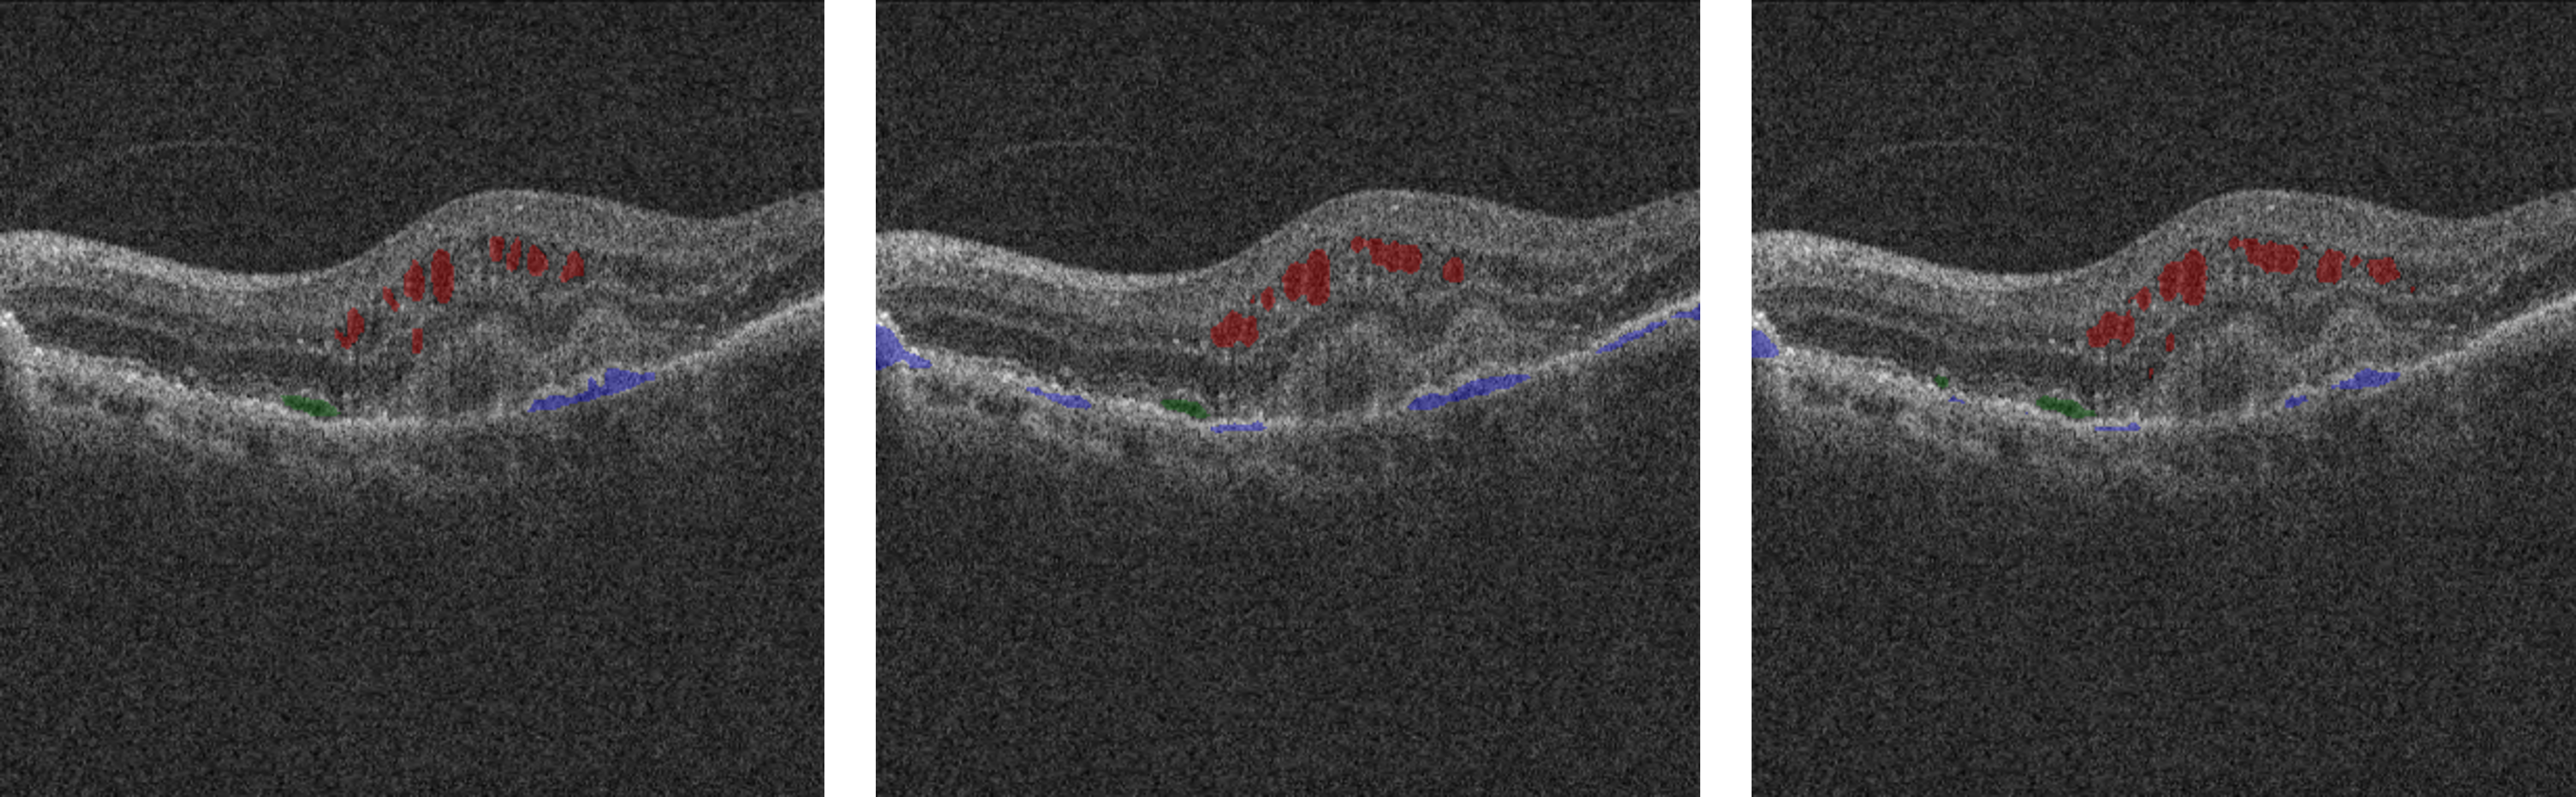
\includegraphics[width=1.0\linewidth]{figures/SegmentationsComparisonBetweenDifferentRotations.png}
	\caption{Predictions by the models trained using $5^{\circ}$ (middle image) and $10^{\circ}$ (right image) rotations, compared with the respective GT (left image).}
	\label{fig:SegmentationsComparisonBetweenDifferentRotations}
\end{figure}

This is an example of how the model trained with $5^{\circ}$ rotations tends to be more conservative in the fluid segmentation, despite not being as good at identifying fluid in the B-scans. For this reason, it was expected that this model would perform better on unseen data than the model trained with $10^{\circ}$ which tends to oversegment. Therefore, the maximum rotation selected for further experiments was $5^{\circ}$.
\par
Following the experiments that applied a $5^{\circ}$ rotation to the seven vertical patches extracted from each B-scan, additional runs were made using the same rotation, but with only four patches extracted from each B-scan instead. The objective of these runs was to verify if model still performs better on seven patches than on four patches when the applied rotation is changed from $10^{\circ}$ to $5^{\circ}$. The results are shown in Table \ref{tab:Experiment1.3FourPatches5DegreeRotation}.

\begin{table*}[!ht]
	\caption{Dice scores for every vendor and fluid using four vertical patches. The rotation applied in these runs was of $5^{\circ}$, instead of the previously used $10^{\circ}$. ``Set 7'' and the best performing run in this set (Run 32) are also shown, promoting an easier comparison between the use of four and seven patches. The underlined values correspond to the best performances between the models trained in Run 32 and Run 33.}
	\centering
	\resizebox{\textwidth}{!}{\begin{tabular}{|c|c|ccc|ccc|ccc|c|c|c|c|}
		\hline
		% Headers
		\multirow{2}{*}{\textbf{Runs}} & 
		\multirow{2}{*}{\textbf{VF}} & 
		\multicolumn{3}{c|}{\textbf{Cirrus}} & 
		\multicolumn{3}{c|}{\textbf{Spectralis}} & 
		\multicolumn{3}{c|}{\textbf{Topcon}} & 
		\multicolumn{1}{c|}{\multirow{2}{*}{\textbf{IRF}}} & 
		\multirow{2}{*}{\textbf{SRF}} & 
		\multirow{2}{*}{\textbf{PED}} & 
		\multirow{2}{*}{\textbf{Fluid}} \\ \cline{3-11} & &
		\multicolumn{1}{c}{\textbf{IRF}} & 
		\multicolumn{1}{c}{\textbf{SRF}} & 
		\textbf{\textbf{PED}} & 
		\multicolumn{1}{c}{\textbf{IRF}} & 
		\multicolumn{1}{c}{\textbf{SRF}} & 
		\textbf{PED} & 
		\textbf{IRF} & 
		\textbf{SRF} & 
		\textbf{PED} & 
		\multicolumn{1}{c|}{} & & & \\ 
			
		\hline
		
		\textbf{Run 33} & 2 & \multicolumn{1}{c|}{0.598} & \multicolumn{1}{c|}{\textbf{0.824}} & 0.719 & \multicolumn{1}{c|}{\textbf{0.805}} & \multicolumn{1}{c|}{0.873} & \underline{\textbf{0.887}} & \multicolumn{1}{c|}{\underline{\textbf{0.848}}} & \multicolumn{1}{c|}{\underline{\textbf{0.947}}} & \underline{\textbf{0.863}} & \textbf{0.720} & \underline{\textbf{0.874}} & \textbf{0.798} & \underline{\textbf{0.733}} \\
		
		\textbf{Run 34} & 3 & \multicolumn{1}{c|}{0.298} & \multicolumn{1}{c|}{0.701} & 0.436 & \multicolumn{1}{c|}{0.442} & \multicolumn{1}{c|}{0.785} & 0.720 & \multicolumn{1}{c|}{0.717} & \multicolumn{1}{c|}{0.814} & 0.746 & 0.477 & 0.757 & 0.599 & 0.530 \\
		
		\textbf{Run 35} & 4 & \multicolumn{1}{c|}{0.670} & \multicolumn{1}{c|}{0.796} & \textbf{0.850} & \multicolumn{1}{c|}{0.531} & \multicolumn{1}{c|}{0.825} & 0.701 & \multicolumn{1}{c|}{0.509} & \multicolumn{1}{c|}{0.703} & 0.674 & 0.582 & 0.759 & 0.754 & 0.578 \\
		
		\textbf{Run 36} & 0 & \multicolumn{1}{c|}{\textbf{0.695}} & \multicolumn{1}{c|}{0.816} & 0.737 & \multicolumn{1}{c|}{0.761} & \multicolumn{1}{c|}{\textbf{0.882}} & 0.838 & \multicolumn{1}{c|}{0.728} & \multicolumn{1}{c|}{0.867} & 0.775 & 0.719 & 0.846 & 0.769 & 0.635 \\
		
		\hline
		
		\textbf{Set 8} & - & \multicolumn{1}{c|}{0.57} & \multicolumn{1}{c|}{\textbf{0.78}} & \textbf{0.69} & \multicolumn{1}{c|}{0.63} & \multicolumn{1}{c|}{0.84} & \textbf{0.79} & \multicolumn{1}{c|}{0.70} & \multicolumn{1}{c|}{\textbf{0.83}} & \textbf{0.76} & 0.62 & \textbf{0.81} & \textbf{0.73} & 0.62 \\
		
		\hline
		\hline
		
		\textbf{Run 32} & 0 & \multicolumn{1}{c|}{\underline{0.794}} & \multicolumn{1}{c|}{\underline{0.878}} & \underline{0.770} & \multicolumn{1}{c|}{\underline{0.807}} & \multicolumn{1}{c|}{\underline{0.902}} & 0.862 & \multicolumn{1}{c|}{0.796} & \multicolumn{1}{c|}{0.842} & 0.830 & \underline{0.797} & 0.869 & \underline{0.808} & 0.698 \\
		
		\hline
		
		\textbf{Set 7} & - & \multicolumn{1}{c|}{\textbf{0.60}} & \multicolumn{1}{c|}{\textbf{0.78}} & 0.68 & \multicolumn{1}{c|}{\textbf{0.71}} & \multicolumn{1}{c|}{\textbf{0.85}} & 0.77 & \multicolumn{1}{c|}{\textbf{0.74}} & \multicolumn{1}{c|}{0.80} & 0.75 & \textbf{0.67} & 0.80 & 0.72 & \textbf{0.63} \\
		
		\hline
			
	\end{tabular}}
	\label{tab:Experiment1.3FourPatches5DegreeRotation}
\end{table*}

Contrasting with the results shown in Table \ref{tab:Experiment1.3FourPatches} and Table \ref{tab:Experiment1.3SevenVsThirteenPatches}, which show a significant improvement when using seven vertical patches over four, the results exhibited in Table \ref{tab:Experiment1.3FourPatches5DegreeRotation} present a similar performance between the models trained on four and seven vertical patches. The main performance differences are in the IRF segmentation, where the difference is more significant depending on the number of patches used, favoring the models trained with seven patches.
\par
However, it is necessary to select a single segmentation model to perform inference in the fold that was reserved. The best performing model from those trained with seven vertical patches obtained from each B-scan and a maximum rotation of $5^{\circ}$ is the model trained in Run 32. Meanwhile, the best performing model from ``Set 8'' is Run 33. In Table \ref{tab:Experiment1.3FourPatches5DegreeRotation}, the underlined values correspond to the best performance attained between Run 32 and 33.
\par
In most metrics, the model trained on Run 32 performs better than the model trained on Run 33. Nevertheless, both performances are really similar in most metrics, with the only significant difference being the IRF segmentation, which is superior in Run 32. It is important to note that the models were nor trained nor validated on the same data and an assumption that this would directly translate to the performance in unseen data was made. However, it is possible that the data in which one model was trained prepares it better for the data on the reserved fold. Therefore, the U-Net model selected to represent the multi-class segmentation approach was the one trained in Run 32. This model subsequently performed the inference in the unseen fold (fold 1) and its results are shown in Table \ref{tab:Experiment1.3FinalResults}. In this table, the rows correspond to the model performances on different sets of slices. In the first row the performance across all slices is considered. In the second row only the slices with the fluid indicated in the column are quantified, while in the third row only those that do not present that fluid are considered.

\begin{table*}[!ht]
	\caption{Dice scores for every vendor and fluid in the reserved fold (fold 1). The first row reports the mean Dice across all slices. The second row shows the mean for slices containing the fluid specified in the column, while the third shows the mean for the slices without that fluid.}
	\centering
	\resizebox{\textwidth}{!}{\begin{tabular}{|c|c|c|ccc|ccc|ccc|c|c|c|c|}
		\hline
		% Headers
		\multirow{2}{*}{\textbf{Runs}} &
		\multirow{2}{*}{\textbf{Slices}} &  
		\multirow{2}{*}{\textbf{VF}} & 
		\multicolumn{3}{c|}{\textbf{Cirrus}} & 
		\multicolumn{3}{c|}{\textbf{Spectralis}} & 
		\multicolumn{3}{c|}{\textbf{Topcon}} & 
		\multicolumn{1}{c|}{\multirow{2}{*}{\textbf{IRF}}} & 
		\multirow{2}{*}{\textbf{SRF}} & 
		\multirow{2}{*}{\textbf{PED}} & 
		\multirow{2}{*}{\textbf{Fluid}} \\ \cline{4-12} & & &
		\multicolumn{1}{c}{\textbf{IRF}} & 
		\multicolumn{1}{c}{\textbf{SRF}} & 
		\textbf{\textbf{PED}} & 
		\multicolumn{1}{c}{\textbf{IRF}} & 
		\multicolumn{1}{c}{\textbf{SRF}} & 
		\textbf{PED} & 
		\textbf{IRF} & 
		\textbf{SRF} & 
		\textbf{PED} & 
		\multicolumn{1}{c|}{} & & & \\ 
			
		\hline
			
		\multirow{3}{*}{\textbf{Run 32}} & All & 1 & \multicolumn{1}{c|}{0.852} & \multicolumn{1}{c|}{0.918} & 0.934 & \multicolumn{1}{c|}{0.645} & \multicolumn{1}{c|}{0.821} & 0.852 & \multicolumn{1}{c|}{0.818} & \multicolumn{1}{c|}{0.929} & 0.755 & 0.799 & 0.905 & 0.841 & 0.742 \\
		
		& Fluid & 1 & \multicolumn{1}{c|}{0.654} & \multicolumn{1}{c|}{0.799} & 0.767 & \multicolumn{1}{c|}{0.645} & \multicolumn{1}{c|}{0.687} & 0.703 & \multicolumn{1}{c|}{0.624} & \multicolumn{1}{c|}{0.744} & 0.588 & 0.641 & 0.756 & 0.716 & 0.702 \\
		
		& No Fluid & 1 & \multicolumn{1}{c|}{0.941} & \multicolumn{1}{c|}{0.972} & 0.978 & \multicolumn{1}{c|}{0.646} & \multicolumn{1}{c|}{0.889} & 0.885 & \multicolumn{1}{c|}{0.884} & \multicolumn{1}{c|}{0.960} & 0.766 & 0.873 & 0.952 & 0.862 & 0.786 \\
		
		\hline
			
	\end{tabular}}
	\label{tab:Experiment1.3FinalResults}
\end{table*}

The results shown in the table indicate that the model generalized well. The performance obtained in the reserved fold, whose data had not been used in training or validation, reveals the model's robustness across different fluids and vendors. Since the model performs equally well across the three vendors, a good cross-device generalization has been achieved. Therefore, the model is not dependent on the image quality of the B-scans to produce accurate predictions.
\par
The model behaved differently depending on the fluid expected to segment. The Dice coefficient was considerably larger in SRF and PED than in IRF. This is associated with the larger variety of IRF shape and position in the retina. IRF regions are usually irregular in shape, smaller, and less well-defined than the other fluids, often appearing as small structures. This fluid is also located between the retinal layers, making it harder for the model to distinguish from the surrounding tissue and often leading to labeling ambiguity. Still, the model attained a better performance in fluid segmentation than those seen in Table \ref{tab:Experiment1.3SevenPatches5DegreeRotationFluid}, where only fluid is considered.
\par
When considering all the slices, the Dice coefficient improves significantly, when compared to its performance where only slices with fluid are considered. At the same time, the Dice coefficient obtained in the slices without fluid is also better than the fluid segmentation. This reflects the greater difficulty of accurately segmenting the fluids, when compared to the task of detecting their presence. Since most slices in the dataset do not present fluid, an accurate detection of it can significantly increase the Dice mean across all slices, as explained previously.
\par
Overall, the performance obtained when validating in this unseen fold is significantly better than any other validation performance in previously seen in Table \ref{tab:Experiment1.3SevenPatches5DegreeRotation}. This indicates that the model did not overfit on training data, benefiting from the diversity introduced in training both through varying images and the transformations applied to them. This performance also benefits from selecting the best performing model in cross-validation, which allows the choice of a robust model. 
\par
In Figures \ref{fig:Experiment1FinalModelPredictionsCirrus}, \ref{fig:Experiment1FinalModelPredictionsSpectralis}, and \ref{fig:Experiment1FinalModelPredictionsTopcon}, some examples of predictions performed by the model in the unseen data are shown. In the IRF segmentations, it is seen that the model can not correctly identify the retinal tissue that separates the fluid regions and connects nearby fluid regions. The PED segmentation is marked by accurate delimitation of the large PED regions, with some predictions made in B-scans without PED. Lastly, SRF is the fluid in which the prediction segmentation more resembles the GT.
\par
The performance seen by this model in the reserved fold was subsequently compared with the best performing models from the following experiment.

\begin{figure}[!ht]
	\centering
	\includegraphics[width=0.9\linewidth]{figures/Experiment1FinalModelPredictionsCirrus.png}
	\caption{Predictions by the model trained on Run 32 in unseen Cirrus volumes of fold 1.}
	\label{fig:Experiment1FinalModelPredictionsCirrus}
\end{figure}

\begin{figure}[!ht]
	\centering
	\includegraphics[width=0.9\linewidth]{figures/Experiment1FinalModelPredictionsSpectralis.png}
	\caption{Predictions by the model trained on Run 32 in unseen Spectralis volumes of fold 1.}
	\label{fig:Experiment1FinalModelPredictionsSpectralis}
\end{figure}

\begin{figure}[!ht]
	\centering
	\includegraphics[width=0.9\linewidth]{figures/Experiment1FinalModelPredictionsTopcon.png}
	\caption{Predictions by the model trained on Run 32 in unseen Topcon volumes of fold 1.}
	\label{fig:Experiment1FinalModelPredictionsTopcon}
\end{figure}

\subsection{Experiment 2 - Fluid Segmentation Using Binary U-Nets}
The results shown in this subsection correspond to the use of three separate U-Nets, one for each fluid, to perform multi-class fluid segmentation. In Experiment 2.1, the loss function was the same as in Experiment 1, while in Experiment 2.2 the loss function was changed to the weighted cross-entropy. The results in these experiments were compared with each other.

\subsubsection{Experiment 2.1 - Multi-class Segmentation Loss}
In this experiment, for each fluid, eight models were trained. One model was trained for each fold in the multi-class 5-fold split and then one model was trained for each fold in a fluid-specific 5-fold split.
\par
Table \ref{tab:Experiment2IRF} illustrates the performance of the models trained to segment IRF, with the upper block corresponding to the models trained on the multi-class split while the second block shows the performances for the models trained on the split specifically made for IRF segmentation.

\begin{table*}[!ht]
	\caption{IRF Dice scores for every vendor. Runs 37 to 40 utilize the multi-class 5-fold split from Experiment 1, while the Runs 41 to 44 use the fluid-specific 5-fold split. The results are presented both for every slice and for the slices which contain IRF.}
	\centering
	\begin{tabular}{|c|c|cc|cc|cc|cc|}
			\hline
			\multirow{2}{*}{\textbf{Runs}} &
			\multirow{2}{*}{\textbf{VF}} & 
			\multicolumn{2}{c|}{\textbf{Cirrus}} & 
			\multicolumn{2}{c|}{\textbf{Spectralis}} & 
			\multicolumn{2}{c|}{\textbf{Topcon}} & 
			\multicolumn{2}{c|}{\textbf{IRF}} \\ 
			\cline{3-10} & &
			\multicolumn{1}{c}{\textbf{All}} &  
			\textbf{\textbf{Fluid}} & 
			\multicolumn{1}{c}{\textbf{All}} &  
			\textbf{\textbf{Fluid}} & 
			\multicolumn{1}{c}{\textbf{All}} & 
			\textbf{\textbf{Fluid}} & 
			\multicolumn{1}{c}{\textbf{All}} & 
			\textbf{\textbf{Fluid}}\\ 
			
			\hline
			
			\textbf{Run 37} & 2 & 0.478 & 0.634 & 0.695 & 0.669 & 0.735 & 0.569 & 0.604 & 0.625 \\
			
			\textbf{Run 38} & 3 & 0.536 & 0.452 & 0.514 & 0.588 & \textbf{0.820} & \textbf{0.706} & 0.637 & 0.553 \\
			
			\textbf{Run 39} & 4 & 0.545 & \textbf{0.683} & 0.617 & 0.670 & 0.540 & 0.484 & 0.552 & 0.600 \\
			
			\textbf{Run 40} & 0 & 0.576 & 0.619 & 0.695 & 0.682 & 0.661 & 0.599 & 0.628 & 0.628 \\
			
			\hline
			
			\textbf{Set 9} & - & 0.53 & 0.60 & 0.63 & 0.65 & 0.69 & \textbf{0.59} & 0.61 & 0.60 \\
			
			\hline
			\hline
			
			\textbf{Run 41} & 2 & \textbf{0.654} & 0.663 & 0.541 & 0.606 & 0.648 & 0.619 & 0.632 & 0.635 \\
			
			\textbf{Run 42} & 3 & 0.507 & 0.641 & \textbf{0.741} & 0.670 & 0.775 & 0.675 & \textbf{0.649} & \textbf{0.656} \\
			
			\textbf{Run 43} & 4 & 0.583 & 0.516 & 0.689 & 0.660 & 0.310 & 0.451 & 0.502 & 0.546 \\
			
			\textbf{Run 44} & 0 & 0.618 & 0.566 & 0.644 & \textbf{0.686} & 0.588 & 0.600 & 0.611 & 0.594 \\
			
			\hline
			
			\textbf{Set 10} & - & 0.59 & 0.60 & 0.65 & \textbf{0.66} & 0.58 & \textbf{0.59} & 0.60 & \textbf{0.61} \\
			
			\hline
			\hline
			
			\textbf{Set 7} & - & \textbf{0.60} & \textbf{0.61} & \textbf{0.71} & 0.65 & \textbf{0.74} & 0.58 & \textbf{0.67} & 0.60 \\
			
			\hline
			
	\end{tabular}
	\label{tab:Experiment2IRF}
\end{table*}

The results shown in this table follow a well defined trend: the IRF segmentation in the slices which contain this fluid performs similarly to the segmentation predicted by multi-class models, while the performance when considering all the slices is significantly worse.
\par
The Dice obtained in segmentation in the slices with IRF is really similar to the values obtained when training multi-class models, as the difference between the mean of the runs performed is around 0.01 for all vendors. Changing the split in which the models were trained barely made a difference in the performances' average. However, while the segmentation in slices with IRF almost did not change, the mean performance in all the slices saw a significant improvement in Cirrus and a slight increase in Spectralis, combined with a significant decrease in Topcon. 
\par
The reason Topcon behaves differently is because, overall, the volumes obtained with devices from this vendor present less fluid than the volumes obtained with the other devices. Therefore, the model has to analyze the Topcon images more carefully and be more attentive of the smaller details, as the fluid regions are not as big as those seen in the other vendors. This leads to the model being better at separating the slices with fluid from those that do not present fluid. As seen in Experiment 1, an effective detection of fluid can significantly improve the model's Dice coefficient. The implications this has in model performance's are also visible in the multi-class segmentation results, as shown in the performance differences in B-scans from Topcon between Table \ref{tab:Experiment1.3SevenPatches5DegreeRotation} and Table \ref{tab:Experiment1.3SevenPatches5DegreeRotationFluid}.
\par
When comparing the results across all slices between these binary models with the multi-class, it is seen a significant decrease in Dice coefficient in the models tasked to segment exclusively IRF. There are two main causes for this decrease, with the first being an increment in the number of pixels labeled as background. As the model attempts to exclusively segment IRF, all the pixels that are not labeled as IRF, are classified as background. This means that the regions of SRF and PED are also interpreted as background. The images in the dataset are predominantly composed of non-fluid pixels, but, by re-assigning the other fluids' pixels in the retina as background, the proportion of fluid pixels in the image, and particularly in the retina, becomes even smaller. As the number of background pixels increase, the more chances the model has of mislabeling them as fluid.
\par
The increased number of background pixels is further impacted with the lack of inter-class competition. This inter-class competition is particularly helpful in the segmentation of other ambiguous regions such as other fluids, which, in binary segmentation, is not contested by other classes. This does not motivate the model to learn the anatomical characteristics of the retina that are key to identifying the region corresponding to each fluid, often leading to over-segmentation. 
\par
This translates to a decrease in the IRF segmentation model's performance, particularly in the slices that do not present this fluid, with two examples shown in Figure \ref{fig:Experiment2IRFSegmentation}. The same performance decrease is also seen in SRF and PED, as shown further, due to the same reasons.

\begin{figure}[!ht]
	\centering
	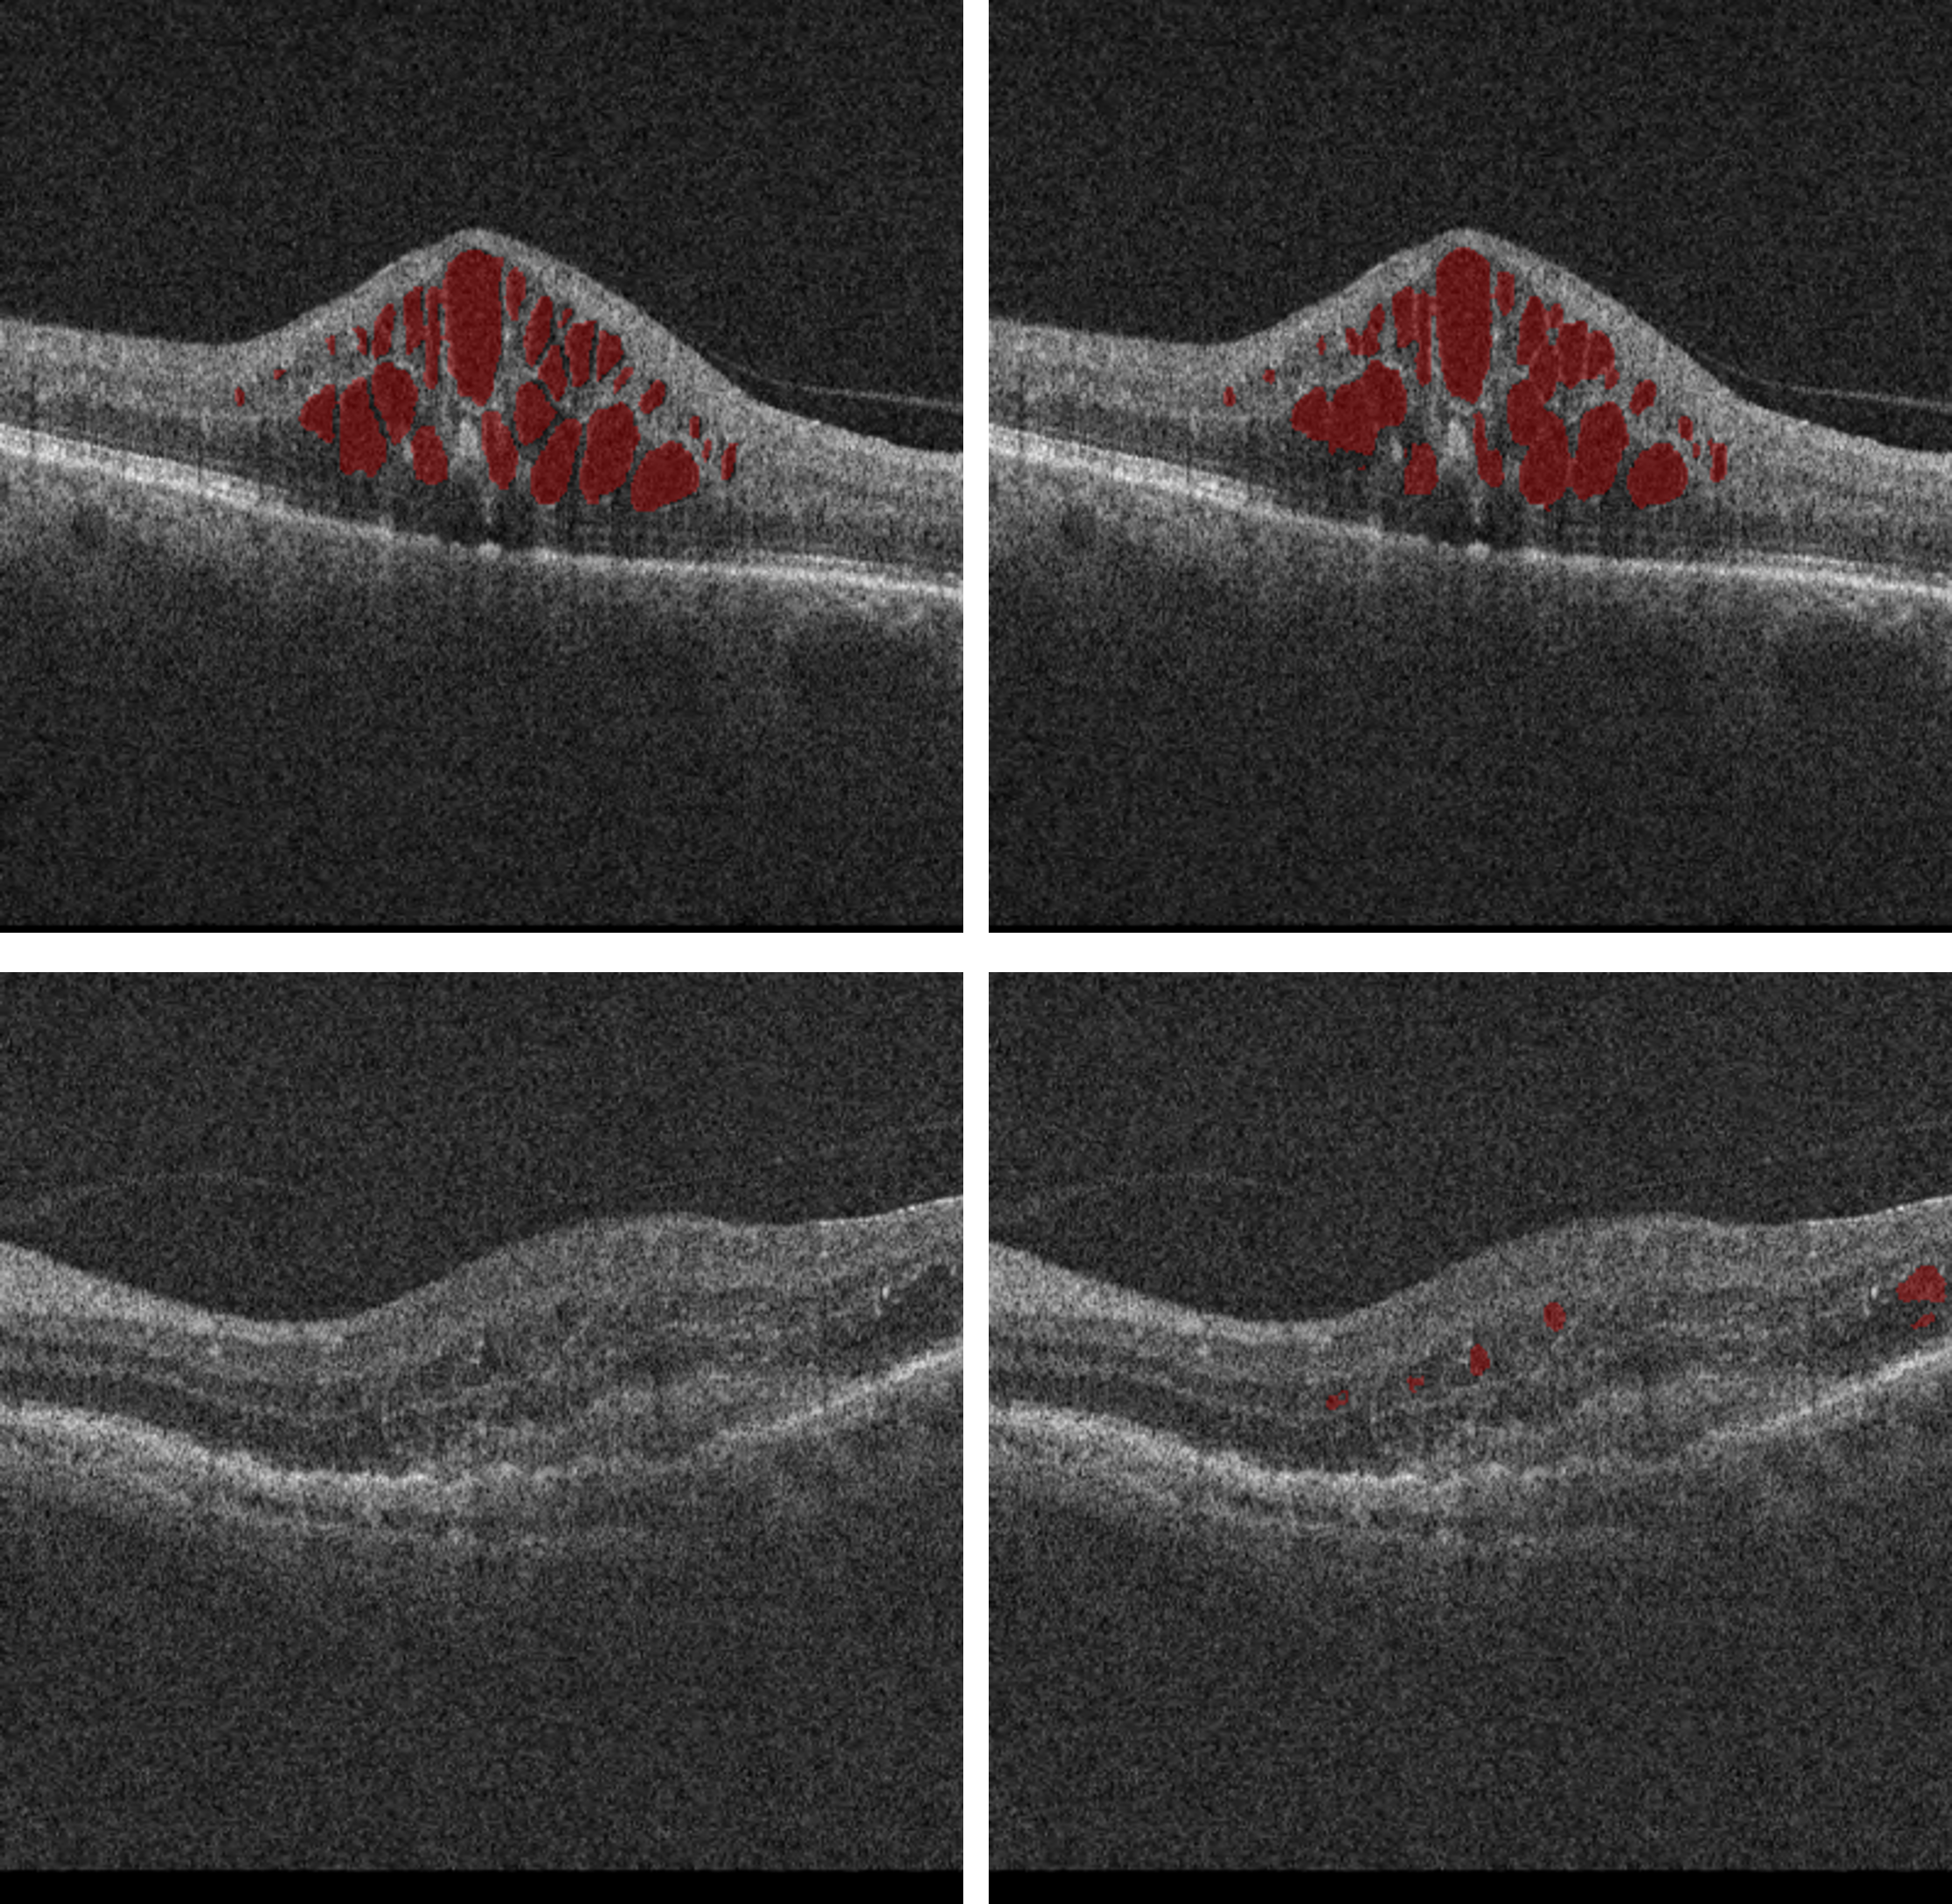
\includegraphics[width=0.7\linewidth]{figures/Experiment2IRFSegmentation.png}
	\caption{Predictions (right) performed by the binary IRF segmentation model and their respective GT (left). The prediction represented in the top show an example of an accurate IRF segmentation, while the bottom prediction reveals an oversegmentation in a slice that does not contain fluid.}
	\label{fig:Experiment2IRFSegmentation}
\end{figure}

Table \ref{tab:Experiment2SRF} shows the performance of the models trained on the same conditions as those trained to segment IRF, but now with the goal of segmenting SRF. Similarly, on the second block of this table, the models were trained using a 5-fold split specifically made to evenly distribute the OCT volumes according to the quantity of SRF in them.

\begin{table*}[!ht]
	\caption{SRF Dice scores for every vendor. Runs 45 to 48 utilize the multi-class 5-fold split from Experiment 1, while the Runs 49 to 52 use the fluid-specific 5-fold split. The results are presented both for every slice and for the slices which present SRF.}
	\centering
	\begin{tabular}{|c|c|cc|cc|cc|cc|}
		\hline
		\multirow{2}{*}{\textbf{Runs}} &
		\multirow{2}{*}{\textbf{VF}} & 
		\multicolumn{2}{c|}{\textbf{Cirrus}} & 
		\multicolumn{2}{c|}{\textbf{Spectralis}} & 
		\multicolumn{2}{c|}{\textbf{Topcon}} & 
		\multicolumn{2}{c|}{\textbf{SRF}} \\ 
		\cline{3-10} & &
		\multicolumn{1}{c}{\textbf{All}} &  
		\textbf{\textbf{Fluid}} & 
		\multicolumn{1}{c}{\textbf{All}} &  
		\textbf{\textbf{Fluid}} & 
		\multicolumn{1}{c}{\textbf{All}} & 
		\textbf{\textbf{Fluid}} & 
		\multicolumn{1}{c}{\textbf{All}} & 
		\textbf{\textbf{Fluid}}\\ 
		
		\hline
		
		\textbf{Run 45} & 2 & \textbf{0.866} & 0.784 & 0.882 & 0.826 & \textbf{0.956} & 0.645 & \textbf{0.899} & 0.774 \\
		
		\textbf{Run 46} & 3 & 0.599 & 0.574 & 0.741 & 0.843 & 0.820 & 0.737 & 0.705 & 0.666 \\
		
		\textbf{Run 47} & 4 & 0.769 & 0.645 & \textbf{0.874} & 0.873 & 0.845 & 0.689 & 0.816 & 0.728 \\
		
		\textbf{Run 48} & 0 & 0.667 & 0.795 & 0.765 & 0.776 & 0.773 & 0.643 & 0.723 & 0.765 \\
		
		\hline
		
		\textbf{Set 11} & - & 0.73 & 0.70 & 0.82 & 0.83 & \textbf{0.85} & 0.68 & 0.79 & 0.73 \\
		
		\hline		
		\hline
		
		\textbf{Run 49} & 2 & 0.509 & 0.758 & 0.617 & 0.793 & 0.759 & 0.607 & 0.613 & 0.745 \\
		
		\textbf{Run 50} & 3 & 0.743 & 0.733 & 0.776 & \textbf{0.885} & 0.901 & 0.801 & 0.807 & 0.779 \\
		
		\textbf{Run 51} & 4 & 0.720 & 0.722 & 0.864 & 0.875 & 0.816 & \textbf{0.803} & 0.781 & 0.809 \\
		
		\textbf{Run 52} & 0 & 0.775 & \textbf{0.872} & 0.810 & 0.826 & 0.879 & 0.676 & 0.819 & \textbf{0.826} \\
		
		\hline
		
		\textbf{Set 12} & - & 0.69 & \textbf{0.77} & 0.77 & 0.84 & 0.84 & \textbf{0.72} & 0.75 & \textbf{0.79} \\
		
		\hline
		\hline
		
		\textbf{Set 7} & - & \textbf{0.78} & 0.74 & \textbf{0.85} & \textbf{0.85} & 0.80 & 0.62 & \textbf{0.80} & 0.75 \\
		
		\hline
		
	\end{tabular}
	\label{tab:Experiment2SRF}
\end{table*}

As seen in this table, the performances in the segmentation of SRF in slices that contain this fluid have attained improved results when compared to those obtained using the multi-class model, especially when using the volume's distribution specific for SRF. In these conditions, the binary model significantly outperformed the multi-class model in the segmentation of slices with SRF from Cirrus and Topcon, while performing almost equally in the Spectralis slices.
\par
When looking at the models trained on the SRF 5-fold split, similarly to what happened in the IRF model, a significant performance decrease is seen when all the slices are considered. In these metrics, the model is outperformed by the multi-class model in every column except in the Topcon slices, where the performance increases. Similar to what was seen in the IRF segmentation, the performances in the Topcon volumes are not affected as much when performing binary segmentation due to the low quantity of fluid present in the OCT scans from this vendor.
\par
The results obtained using the multi-class split follow the same trend in Topcon. However, in Cirrus, it is seen a small increase in the Dice coefficient when considering all the slices. This is caused by the not so even volumes distribution, resulting in some folds having easier volumes for fluid detection, which have less fluid. This reflects in the high variance seen in the performance considering all slices in Cirrus. Contrasting, when the data is split equally, the dispersion is less pronounced, with only one outlier in that device (Run 49). Despite being more noticeable in Cirrus, Spectralis presents the same issue, where the results when using the multi-class split differ from what is expected and have sparser values.
\par
Overall, the Dice coefficient obtained in the SRF binary segmentation is better than the Dice obtained in the IRF. This same trend is also seen in Experiment 1, where SRF is the best performing fluid.
\par
The runs in which a binary segmentation U-Net was trained to segment PED are shown in Table \ref{tab:Experiment2PED}, where the behavior is comparable with the ones seen in IRF and SRF.

\begin{table*}[!ht]
	\caption{PED Dice scores for every vendor. Runs 53 to 56 utilize the multi-class 5-fold split from Experiment 1, while the Runs 57 to 60 use the fluid-specific 5-fold split. The results are presented both for every slice and for the slices which present PED.}
	\centering
	\begin{tabular}{|c|c|cc|cc|cc|cc|}
		\hline
		\multirow{2}{*}{\textbf{Runs}} &
		\multirow{2}{*}{\textbf{VF}} & 
		\multicolumn{2}{c|}{\textbf{Cirrus}} & 
		\multicolumn{2}{c|}{\textbf{Spectralis}} & 
		\multicolumn{2}{c|}{\textbf{Topcon}} & 
		\multicolumn{2}{c|}{\textbf{PED}} \\ 
		\cline{3-10} & &
		\multicolumn{1}{c}{\textbf{All}} &  
		\textbf{\textbf{Fluid}} & 
		\multicolumn{1}{c}{\textbf{All}} &  
		\textbf{\textbf{Fluid}} & 
		\multicolumn{1}{c}{\textbf{All}} & 
		\textbf{\textbf{Fluid}} & 
		\multicolumn{1}{c}{\textbf{All}} & 
		\textbf{\textbf{Fluid}}\\ 
		
		\hline
		
		\textbf{Run 53} & 2 & 0.305 & 0.482 & 0.555 & 0.623 & 0.626 & 0.552 & 0.459 & 0.522 \\
		
		\textbf{Run 54} & 3 & 0.447 & 0.508 & 0.437 & 0.628 & \textbf{0.769} & 0.623 & 0.563 & 0.583 \\
		
		\textbf{Run 55} & 4 & 0.368 & 0.594 & 0.346 & 0.566 & 0.328 & 0.618 & 0.348 & 0.600 \\
		
		\textbf{Run 56} & 0 & 0.484 & 0.547 & 0.326 & 0.639 & 0.697 & 0.460 & 0.534 & 0.545 \\
		
		\hline
		
		\textbf{Set 13} & - & 0.40 & 0.53 & 0.42 & 0.61 & 0.61 & 0.56 & 0.48 & 0.56 \\
		
		\hline
		\hline
		
		\textbf{Run 57} & 2 & 0.357 & 0.561 & 0.304 & 0.720 & 0.456 & 0.593 & 0.381 & 0.594 \\
		
		\textbf{Run 58} & 3 & 0.232 & 0.581 & 0.305 & 0.574 & 0.361 & 0.568 & 0.292 & 0.574 \\
		
		\textbf{Run 59} & 4 & 0.456 & \textbf{0.648} & 0.345 & 0.601 & 0.588 & \textbf{0.775} & 0.499 & \textbf{0.703} \\
		
		\textbf{Run 60} & 0 & \textbf{0.515} & 0.620 & \textbf{0.558} & \textbf{0.769} & 0.672 & 0.529 & \textbf{0.580} & 0.630 \\
		
		\hline
		
		\textbf{Set 14} & - & 0.39 & \textbf{0.60} & 0.38 & \textbf{0.67} & 0.52 & \textbf{0.62} & 0.44 & \textbf{0.63} \\
		
		\hline
		\hline
		
		\textbf{Set 7} & - & \textbf{0.68} & 0.59 & \textbf{0.77} & 0.65 & \textbf{0.75} & 0.55 & \textbf{0.72} & 0.59 \\
		
		\hline
		
	\end{tabular}
	\label{tab:Experiment2PED}
\end{table*}

In the binary segmentation of PED, the Dice coefficients obtained in the segmentation of slices with this fluid attained slightly better results when compared with those obtained in Experiment 1. However, this is only true when using the 5-fold split specifically made for this fluid. As seen in the previous experiments, the performance declines when considering all the slices.
\par
In the context of PED, it is important to understand the distribution of the fluid across the OCT volumes. While in IRF and SRF all volumes contain at least one of these fluids, in varying quantities, PED appears only in a smaller number of volumes and, in general, in large quantities. This makes the fair division across folds harder, since in each fold the B-scans that compose it are either with a large deformation caused by PED or, in most cases, without PED at all. This happens because most of the OCT volumes that present PED are in severe cases, where large quantities of all fluids appear. This large intra-class variability significantly affects the performance as it increases the difficulty of segmentation, leading to multiple occurrences of oversegmentation.
\par
This uneven distribution contributes to a poor performance when using all slices. It was already exposed that the models attained better fluid detection when dealing with smaller quantities of fluid, which resulted in a better detection performance in Topcon, where IRF and SRF appear in smaller areas. Now, when dealing with PED, the same trend is seen. However, in the other vendors, where PED appears in a larger quantity, the regions with this fluid generally occupy either larger areas or do not appear at all. This confuses the models, often leading to a segmentation of PED in slices where it is not present. This issue did not affect multi-class segmentation as the model capability of understanding the retina anatomy was more developed, as it was required to attribute the correct label to each pixel, which motivated the association between PED regions and the deformations seen in the retina.
\par
This translates to a good performance in the slices with fluid, but poor performance when all slices are considered. When the data partition is made specifically for PED, the quantity of fluid is fair in training and validation and the performances tend to what is expected: a significant decrease when all slices are considered, when compared to the segmentation in the slices with fluid, where the performance is decent. When using the multi-class segmentation split, fluid is not as evenly distributed, resulting in folds with more slices with PED and other folds with more slices without this fluid. In this case, and particularly in Topcon, models trained in folds that contain less fluid perform better at detecting fluid. For example, in Run 54, the models are trained on Topcon volumes with lower quantities of PED while fold 4 contains larger amounts, leading to correct detection of fluid in B-scans without any pixels labeled with this fluid. Inversely, in Run 55, the validation fold is composed of Topcon volumes with small amounts of PED, but trained on volumes with larger quantities. This results in oversegmentation in validation, thus attaining small Dice values when considering all the slices, but a decent score in the slices that have PED. Two examples of the segmentation performed by the binary PED model are shown in Figure \ref{fig:Experiment2PEDSegmentation}.

\begin{figure}[!ht]
	\centering
	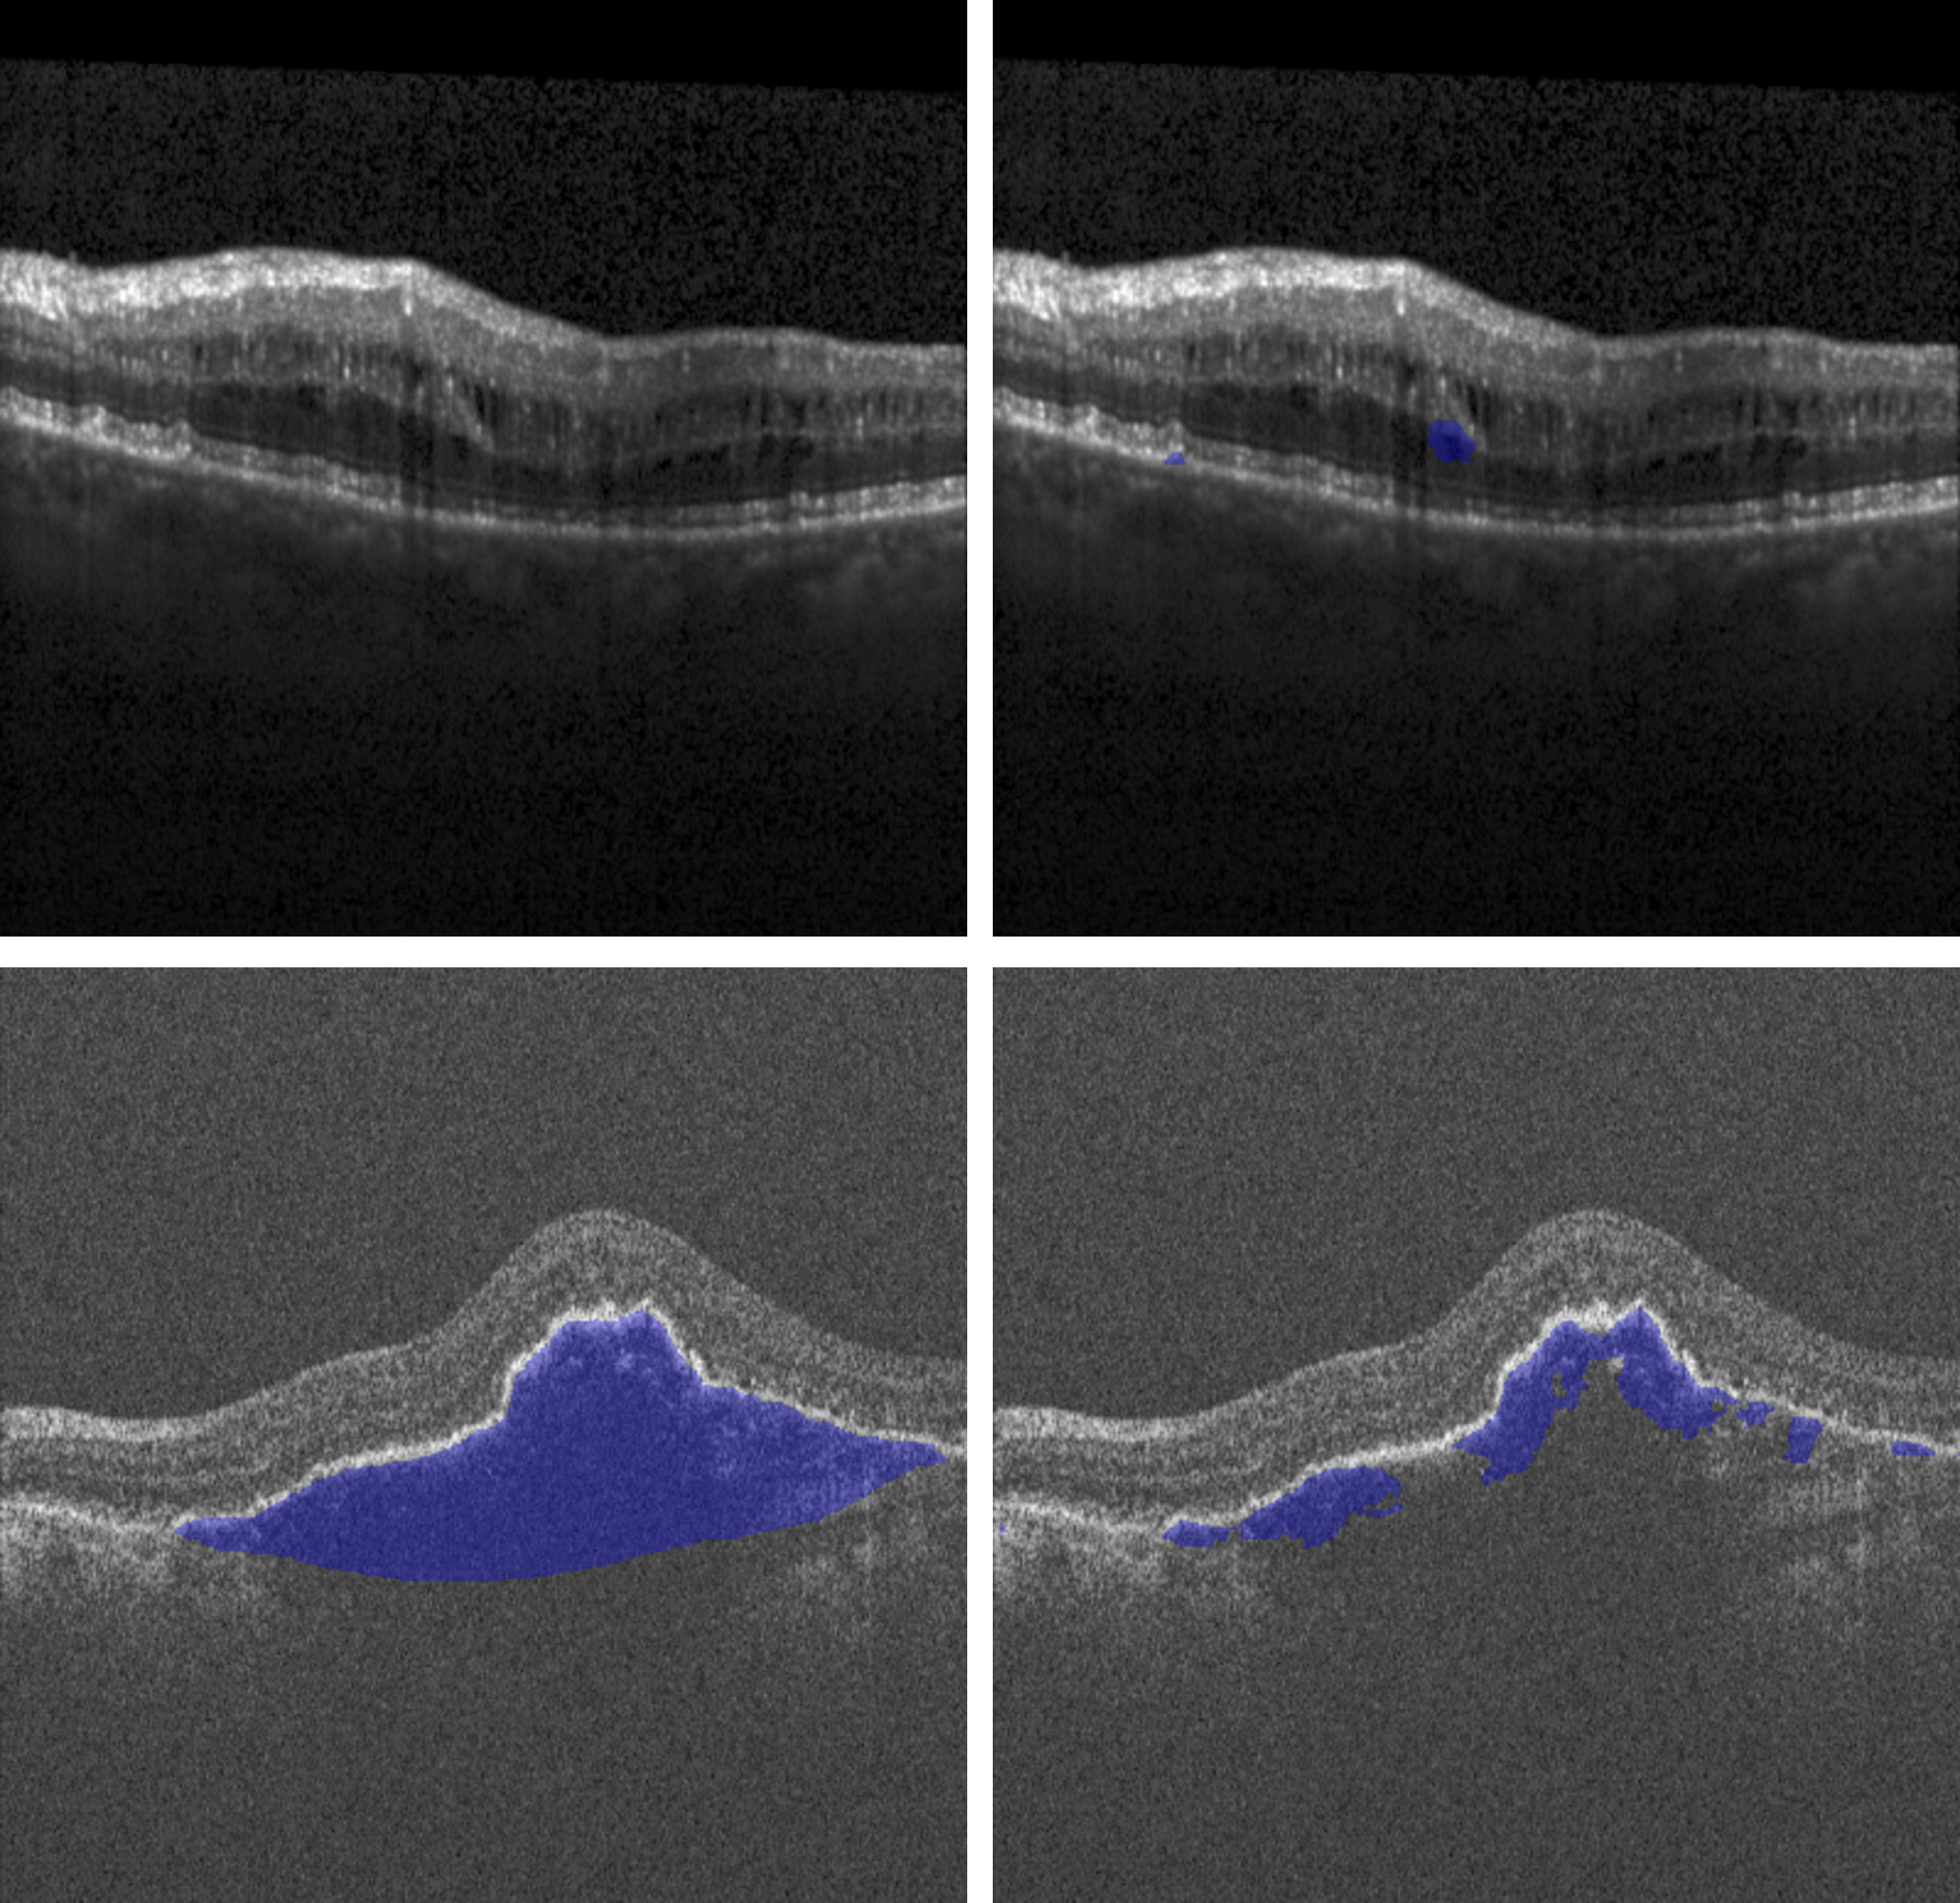
\includegraphics[width=0.7\linewidth]{figures/Experiment2PEDSegmentation.png}
	\caption{Predictions (right) performed by the binary PED segmentation model and their respective GT (left). In top right, the model predicted PED fluid in a region where it does not exist. The bottom images show the undersegmentation of the model trained in Run 59. While this model is capable of detecting the fluid location, it fails to segment its entirety.}
	\label{fig:Experiment2PEDSegmentation}
\end{figure}

In order to compare the results from this Experiment to the ones obtained in Experiment 1, three models had to be selected: one for IRF, one for SRF, and one for PED. Since the results obtained in Experiment 2.2 were much worse than the results reached in this experiment, the models selected for the inference in the unseen fold were selected from the runs performed in Experiment 2.1.
\par
From the models trained for IRF segmentation, ranging from Run 37 to Run 44, the model which obtained the best performance was the one trained on Run 42, as seen in Table \ref{tab:Experiment2IRF}. This model reached the best average performance in the segmentation of IRF both in all slices and when only slices with IRF were considered. In the other metrics, this model's performance were consistently similar to the best performing model in each metric. When compared to the average model from ``Set 7'', this model reached better performances in most metrics.
\par
The model selected to infer the SRF masks in the unseen fold was the model trained on Run 52. This model was the best performing SRF model in fluid segmentation in slices where SRF is present. In the other metrics, it performed closely to the best models, surpassing the average model from ``Set 7'' in most metrics.
\par
In PED, the selected model was the one trained on Run 59. This model was the best model in PED segmentation in slices that contain this fluid, with a significant difference from the other models. When considering all the slices, the model was the second best, but with a weak performance. Regarding the slices with fluid, this model outperformed the average from ``Set 7'' in all vendors. However, similar to all the other models trained for the binary segmentation of PED, it achieved a significantly worse performance when compared to the ones obtained in multi-class.
\par
When merging the masks from three independent binary segmentation models with the goal of outputting a multi-class segmentation, overlaps may occur, where multiple models assign different fluid labels to the same pixel. To resolve this conflict, two alternatives were explored in this fold: a priority-based approach, where the SRF takes precedence over IRF, which in turn takes precedence over PED; and a probability-based approach, where the predicted probabilities for the pixel are compared, attributing the label with highest predicted probability to it. An example of merging using probability-based approach compared to the priority based approach is seen in Figure .

\begin{figure}[!ht]
	\centering
	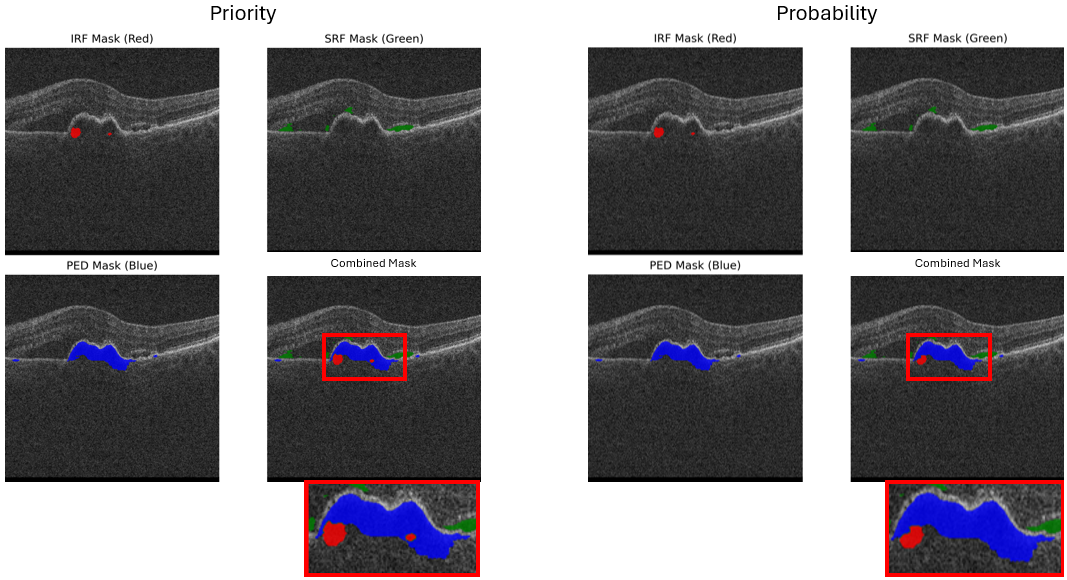
\includegraphics[width=1.0\linewidth]{figures/ProbabilityVsPrioritySegmentation.png}
	\caption{Comparison between the priority (left) and probability (right) merging approach.}
	\label{fig:ProbabilityVsPrioritySegmentation}
\end{figure}

The results obtained using the three selected models are shown in Table \ref{tab:Experiment2FinalResults}, where the first block corresponds to the results when using the priority-based merging approach and the second block presents the results when using the probability-based approach.

\begin{table*}[!ht]
	\caption{Dice scores for every vendor and fluid in the reserved fold (fold 1), using the models from Runs 42, for IRF, 52, for SRF, and 59, for PED. The first block corresponds to the results when using the priority rule merging strategy, while the second block is associated with the results when using highest probability as the merging strategy. In each block, the first row reports the mean Dice across all slices. The second row shows the mean for slices containing the fluid specified in the column, while the third shows the mean for the slices without that fluid. The values marked in bold are the best values when corresponding rows are compared, so that, for example, the row ``All'' in the first block is compared to the row of same name in the second.}
	\centering
	\resizebox{\textwidth}{!}{\begin{tabular}{|c|c|c|ccc|ccc|ccc|c|c|c|c|}
			\hline
			% Headers
			\multirow{2}{*}{\textbf{Runs}} &
			\multirow{2}{*}{\textbf{Slices}} &  
			\multirow{2}{*}{\textbf{VF}} & 
			\multicolumn{3}{c|}{\textbf{Cirrus}} & 
			\multicolumn{3}{c|}{\textbf{Spectralis}} & 
			\multicolumn{3}{c|}{\textbf{Topcon}} & 
			\multicolumn{1}{c|}{\multirow{2}{*}{\textbf{IRF}}} & 
			\multirow{2}{*}{\textbf{SRF}} & 
			\multirow{2}{*}{\textbf{PED}} & 
			\multirow{2}{*}{\textbf{Fluid}} \\ \cline{4-12} & & &
			\multicolumn{1}{c}{\textbf{IRF}} & 
			\multicolumn{1}{c}{\textbf{SRF}} & 
			\textbf{\textbf{PED}} & 
			\multicolumn{1}{c}{\textbf{IRF}} & 
			\multicolumn{1}{c}{\textbf{SRF}} & 
			\textbf{PED} & 
			\textbf{IRF} & 
			\textbf{SRF} & 
			\textbf{PED} & 
			\multicolumn{1}{c|}{} & & & \\ 
			
			\hline
			
			\multirow{3}{*}{\parbox{2cm}{\textbf{Runs 42, 52, and 59}}} & All & 1 & \multicolumn{1}{c|}{0.693} & \multicolumn{1}{c|}{0.776} & 0.425 & \multicolumn{1}{c|}{0.587} & \multicolumn{1}{c|}{0.623} & 0.177 & \multicolumn{1}{c|}{0.808} & \multicolumn{1}{c|}{0.858} & \textbf{0.531} & 0.723 & 0.783 & 0.425 & \textbf{0.544} \\
			
			& Fluid & 1 & \multicolumn{1}{c|}{0.687} & \multicolumn{1}{c|}{\textbf{0.670}} & 0.573 & \multicolumn{1}{c|}{\textbf{0.660}} & \multicolumn{1}{c|}{\textbf{0.659}} & 0.632 & \multicolumn{1}{c|}{\textbf{0.634}} & \multicolumn{1}{c|}{\textbf{0.560}} & \textbf{0.484} & \textbf{0.661} & \textbf{0.640} & 0.570 & \textbf{0.639} \\
			
			& No Fluid & 1 & \multicolumn{1}{c|}{0.695} & \multicolumn{1}{c|}{0.824} & \textbf{0.387} & \multicolumn{1}{c|}{\textbf{0.520}} & \multicolumn{1}{c|}{0.605} & \textbf{0.075} & \multicolumn{1}{c|}{0.867} & \multicolumn{1}{c|}{0.907} & \textbf{0.534} & 0.752 & 0.830 & \textbf{0.402} & \textbf{0.440} \\
			
			\hline
			\hline
			
			\multirow{3}{*}{\parbox{2cm}{\textbf{Runs 42, 52, and 59}}} & All & 1 & \multicolumn{1}{c|}{\textbf{0.697}} & \multicolumn{1}{c|}{\textbf{0.787}} & \textbf{0.428} & \multicolumn{1}{c|}{\textbf{0.628}} & \multicolumn{1}{c|}{\textbf{0.631}} & \textbf{0.178} & \multicolumn{1}{c|}{\textbf{0.810}} & \multicolumn{1}{c|}{\textbf{0.864}} & \textbf{0.531} & \textbf{0.733} & \textbf{0.792} & \textbf{0.427} & \textbf{0.544} \\
			
			& Fluid & 1 & \multicolumn{1}{c|}{\textbf{0.688}} & \multicolumn{1}{c|}{0.663} & \textbf{0.586} & \multicolumn{1}{c|}{\textbf{0.660}} & \multicolumn{1}{c|}{0.646} & \textbf{0.636} & \multicolumn{1}{c|}{0.632} & \multicolumn{1}{c|}{0.537} & \textbf{0.484} & \textbf{0.661} & 0.627 & \textbf{0.578} & \textbf{0.639} \\
			
			& No Fluid & 1 & \multicolumn{1}{c|}{\textbf{0.701}} & \multicolumn{1}{c|}{\textbf{0.844}} & \textbf{0.387} & \multicolumn{1}{c|}{\textbf{0.520}} & \multicolumn{1}{c|}{\textbf{0.623}} & \textbf{0.075} & \multicolumn{1}{c|}{\textbf{0.870}} & \multicolumn{1}{c|}{\textbf{0.917}} & \textbf{0.534} & \textbf{0.766} & \textbf{0.844} & \textbf{0.402} & \textbf{0.440} \\
			
			\hline
			
	\end{tabular}}
	\label{tab:Experiment2FinalResults}
\end{table*}

The performances of the models shown in this table, indicate that the best merging strategy is the probability-based. In the slices that contain the evaluated fluid, the priority-based approach performs better in SRF, since it is the fluid of highest priority. Regarding IRF, in the slices where this fluid is present, the performance is equal for both approaches, while in PED the probability-based approach is better.
\par
However, when considering all the slices, the approach based on the probability of each model is significantly better. This is tied to the better performance in the slices that do not contain at least on type of fluid. In these slices, this approach prevents the segmentation of the fluids which are not present in the slice. These oversegmentations can be wrongfully predicted in the region of other fluids. However, since the models responsible for correctly segmenting this region are more confident than the models that are wrongfully segmenting it, the labels are attributed to the correct class.
\par
It is important to note that the ``Fluid'' column does not change when using different merging approaches. This is because the region of fluid segmented stays the same, since the only changes performed are in pixels contested by multiple fluids, and if all the fluids belonged to a single class, as considered in this column, no changes would be made.
\par
The overall segmentation performance was comparable to the values obtained in the validation folds, during training. In IRF, the model trained in Run 42 reaches better results in this unseen fold than in the fold in which it was originally validated. This is true when considering all the slices, just those with IRF, or the slices without IRF, which signals the good generalization by the model.
\par
In the segmentation of SRF, the model did not perform as good in this fold. The fluid detection was better, seen by the significant increase in Dice coefficient when considering all the slices instead of just those with fluid, which opposes the results obtained in the validation in Run 52, where the performance decreases in this situation. However, the segmentation worsened significantly in the slices with SRF, as the Dice coefficient dropped from 0.819 in its original validation fold to 0.627. Nevertheless, when considering all the slices, the Dice coefficients are still similar, largely due to the improved Dice in the slices without SRF.
\par
When segmenting IRF and SRF, the models benefited from a good generalization in fluid detection task, which surpassed the performances originally obtained in validation. However, in PED, where the models were the most sensitive in this matter, the performance in this task was worse. It is the only fluid in which the Dice is worse when considering all the slices than when considering just the slices with the fluid. This performance is tied to the model selected for PED segmentation. As seen in Table \ref{tab:Experiment2PED}, the model trained in Run 59 already presents a subpar performance in fluid detection, seen by the decrease in Dice coefficient when considering all the slices instead of those that contain PED. Therefore, the poor detection in unseen images is not unexpected. Note that the model selected detects fluid worse in the Spectralis volumes, similar to what was seen in the model validation. Similarly, the vendor in which the best performance is attained is the Topcon, where the model also performed best during validation. Moreover, all the PED models were expected to generalize worse in the unseen fold in the fluid detection task, due to the reasons previously presented that justify the lack of robustness in these models, such as the heterogeneous distribution of PED in OCT volumes.
\par
In Figures \ref{fig:Experiment2FinalModelPredictionsCirrus}, \ref{fig:Experiment2FinalModelPredictionsSpectralis}, and \ref{fig:Experiment2FinalModelPredictionsTopcon}, it is possible to see the predictions made by the multi-class segmentation performed by binary models specific for each fluid, in Cirrus, Spectralis, and Topcon, respectively. The B-scans presented in these figures are the same as those shown in Experiment 1. In the first row, the GT of each B-scans segmentation is shown, while in the second row the segmentations were performed by the best multi-class model selected in Experiment 1. In the last row, the predictions made by the best models from Experiment 2 are shown.

\begin{figure}[!ht]
	\centering
	\includegraphics[width=0.7\linewidth]{figures/Experiment2FinalModelPredictionsCirrus.png}
	\caption{Predictions by the models trained on Run 42, 52, and 59 in unseen Cirrus volumes of fold 1 (last row), contrasting with predictions made by the multi-class model from Experiment 1.}
	\label{fig:Experiment2FinalModelPredictionsCirrus}
\end{figure}

\begin{figure}[!ht]
	\centering
	\includegraphics[width=0.7\linewidth]{figures/Experiment2FinalModelPredictionsSpectralis.png}
	\caption{Predictions by the models trained on Run 42, 52, and 59 in unseen Spectralis volumes of fold 1 (last row), contrasting with predictions made by the multi-class model from Experiment 1.}
	\label{fig:Experiment2FinalModelPredictionsSpectralis}
\end{figure}

\begin{figure}[!ht]
	\centering
	\includegraphics[width=0.7\linewidth]{figures/Experiment2FinalModelPredictionsTopcon.png}
	\caption{Predictions by the models trained on Run 42, 52, and 59 in unseen Topcon volumes of fold 1 (last row), contrasting with predictions made by the multi-class model from Experiment 1.}
	\label{fig:Experiment2FinalModelPredictionsTopcon}
\end{figure}

\subsubsection{Experiment 2.2 - Balanced Cross-entropy Loss}

In this experiment, the loss function used in the training of the segmentation models was changed from a combination of a weighted cross-entropy and Dice coefficient of the foreground to the weighted cross-entropy. The results are shown in Table \ref{tab:Experiment2.2Results}, where only two runs were performed for the segmentation of IRF, one in each 5-fold split. 

\begin{table*}[!ht]
	\caption{IRF Dice scores for every vendor, using the binary segmentation U-Net for IRF. The loss function used in Runs 61 and 62 is the weighted cross-entropy. This model was trained on two different validation folds: validation fold 0 from the multi-class 5-fold split, and validation fold 4 from the 5-fold split specific for IRF. These results can be compared, respectively, to those obtained in Runs 40 and 43. The metrics are compared between rows with the same name, so that the values in bold are the best across the four experiments.}
	\centering
	\begin{tabular}{|c|c|c|c|c|c|c|}
			\hline
			% Headers
			\textbf{Runs} &
			\textbf{Slices} &  
			\textbf{VF} & 
			\textbf{Cirrus} & 
			\textbf{Spectralis} & 
			\textbf{Topcon} & 
			\textbf{IRF} \\ 
			
			\hline
			
			\multirow{3}{*}{\textbf{Run 61}} & All & 0 & 0.088 & 0.164 & 0.121 & 0.113 \\
			
			& Fluid & 0 & 0.320 & 0.390 & 0.472 & 0.378 \\
			
			& No Fluid & 0 & 0.002 & 0.044 & 0.041 & 0.024 \\
			
			\hline
			
			\multirow{3}{*}{\textbf{Run 62}} & All & 4 & 0.130 & 0.250 & 0.142 & 0.151 \\
			
			& Fluid & 4 & 0.399 & 0.531 & 0.549 & 0.466 \\
						
			& No Fluid & 4 & 0.000 & 0.052 & 0.053 & 0.030 \\
			
			\hline
			\hline
			
			\multirow{3}{*}{\textbf{Run 40}} & All & 0 & 0.576 & \textbf{0.695} & \textbf{0.661} & \textbf{0.628} \\
			
			& Fluid & 0 & \textbf{0.619} & \textbf{0.682} & \textbf{0.599} & \textbf{0.628} \\
			
			& No Fluid & 0 & 0.555 & 0.705 & \textbf{0.686} & \textbf{0.628} \\
			
			\hline
			
			\multirow{3}{*}{\textbf{Run 43}} & All & 4 & \textbf{0.583} & 0.689 & 0.310 & 0.502 \\
			
			& Fluid & 4 & 0.516 & 0.660 & 0.451 & 0.546 \\
			
			& No Fluid & 4 & \textbf{0.601} & \textbf{0.719} & 0.272 & 0.486 \\
			
			\hline
			
	\end{tabular}
	\label{tab:Experiment2.2Results}
\end{table*}

The results seen in the table are much worse than those obtained in the same conditions with the previous loss. In the slices with IRF, the segmentation was poor, but with a performance almost comparable to the values obtained in Run 40 and 43.
\par
However, what really worsens the overall performance is fluid detection. All the Dice coefficients in the slices with no fluid were inferior than 0.05, while most of the models studied in Experiment 2.1 reached values superior than 0.5.
\par
The reason these values were so low is related with the loss function used. By keeping the Dice loss as a component of the training loss, the model is highly penalized when predicting fluid in an image which does not have fluid. Whenever any fluid is predicted in such image, the Dice coefficient is 0. This motivates the model to carefully predict pixels in regions of the image where it highly believes there is fluid.
\par
When removing the Dice component from the loss, the wrongful predictions are only penalized by the cross-entropy component. This component does not penalize as much the predictions of fluid in empty images. The cross-entropy of each B-scan is calculated adjusted to the number of pixels belonging to a class in the image, as shown in \ref{Methods} Materials and Methods. Whenever a background pixel is wrongfully classified as fluid, the resulting penalty is really small, due to the large quantity of background pixels in the mask. Therefore, the motivation to not segment fluid in images which are solely composed of background is much smaller than it is when the Dice is considered. This results in segmentations such as the one seen in Figure \ref{fig:BCESegmentationError}.
\par
The cross-entropy is much more useful when regularizing the wrong labeling, especially in fluid. Since this loss component is adjusted to the representation of each class in the image, wrongfully labeling a fluid region as another fluid or background brings a large penalty to the model. This is why it is combined with the Dice loss in the original loss: while the Dice ensures that the correct areas of fluid are segmented, the cross-entropy makes sure that the correct labels are assigned to each pixel. For this reason, most of the segmentation errors that are seen in the predictions made by the models trained in Run 61 and 62 are oversegmentations, and not as many incorrect labelings. An example of how this translates to the model's segmentation is seen in Figure \ref{fig:BCESegmentationDecent}.

\begin{figure}[!ht]
	\centering
	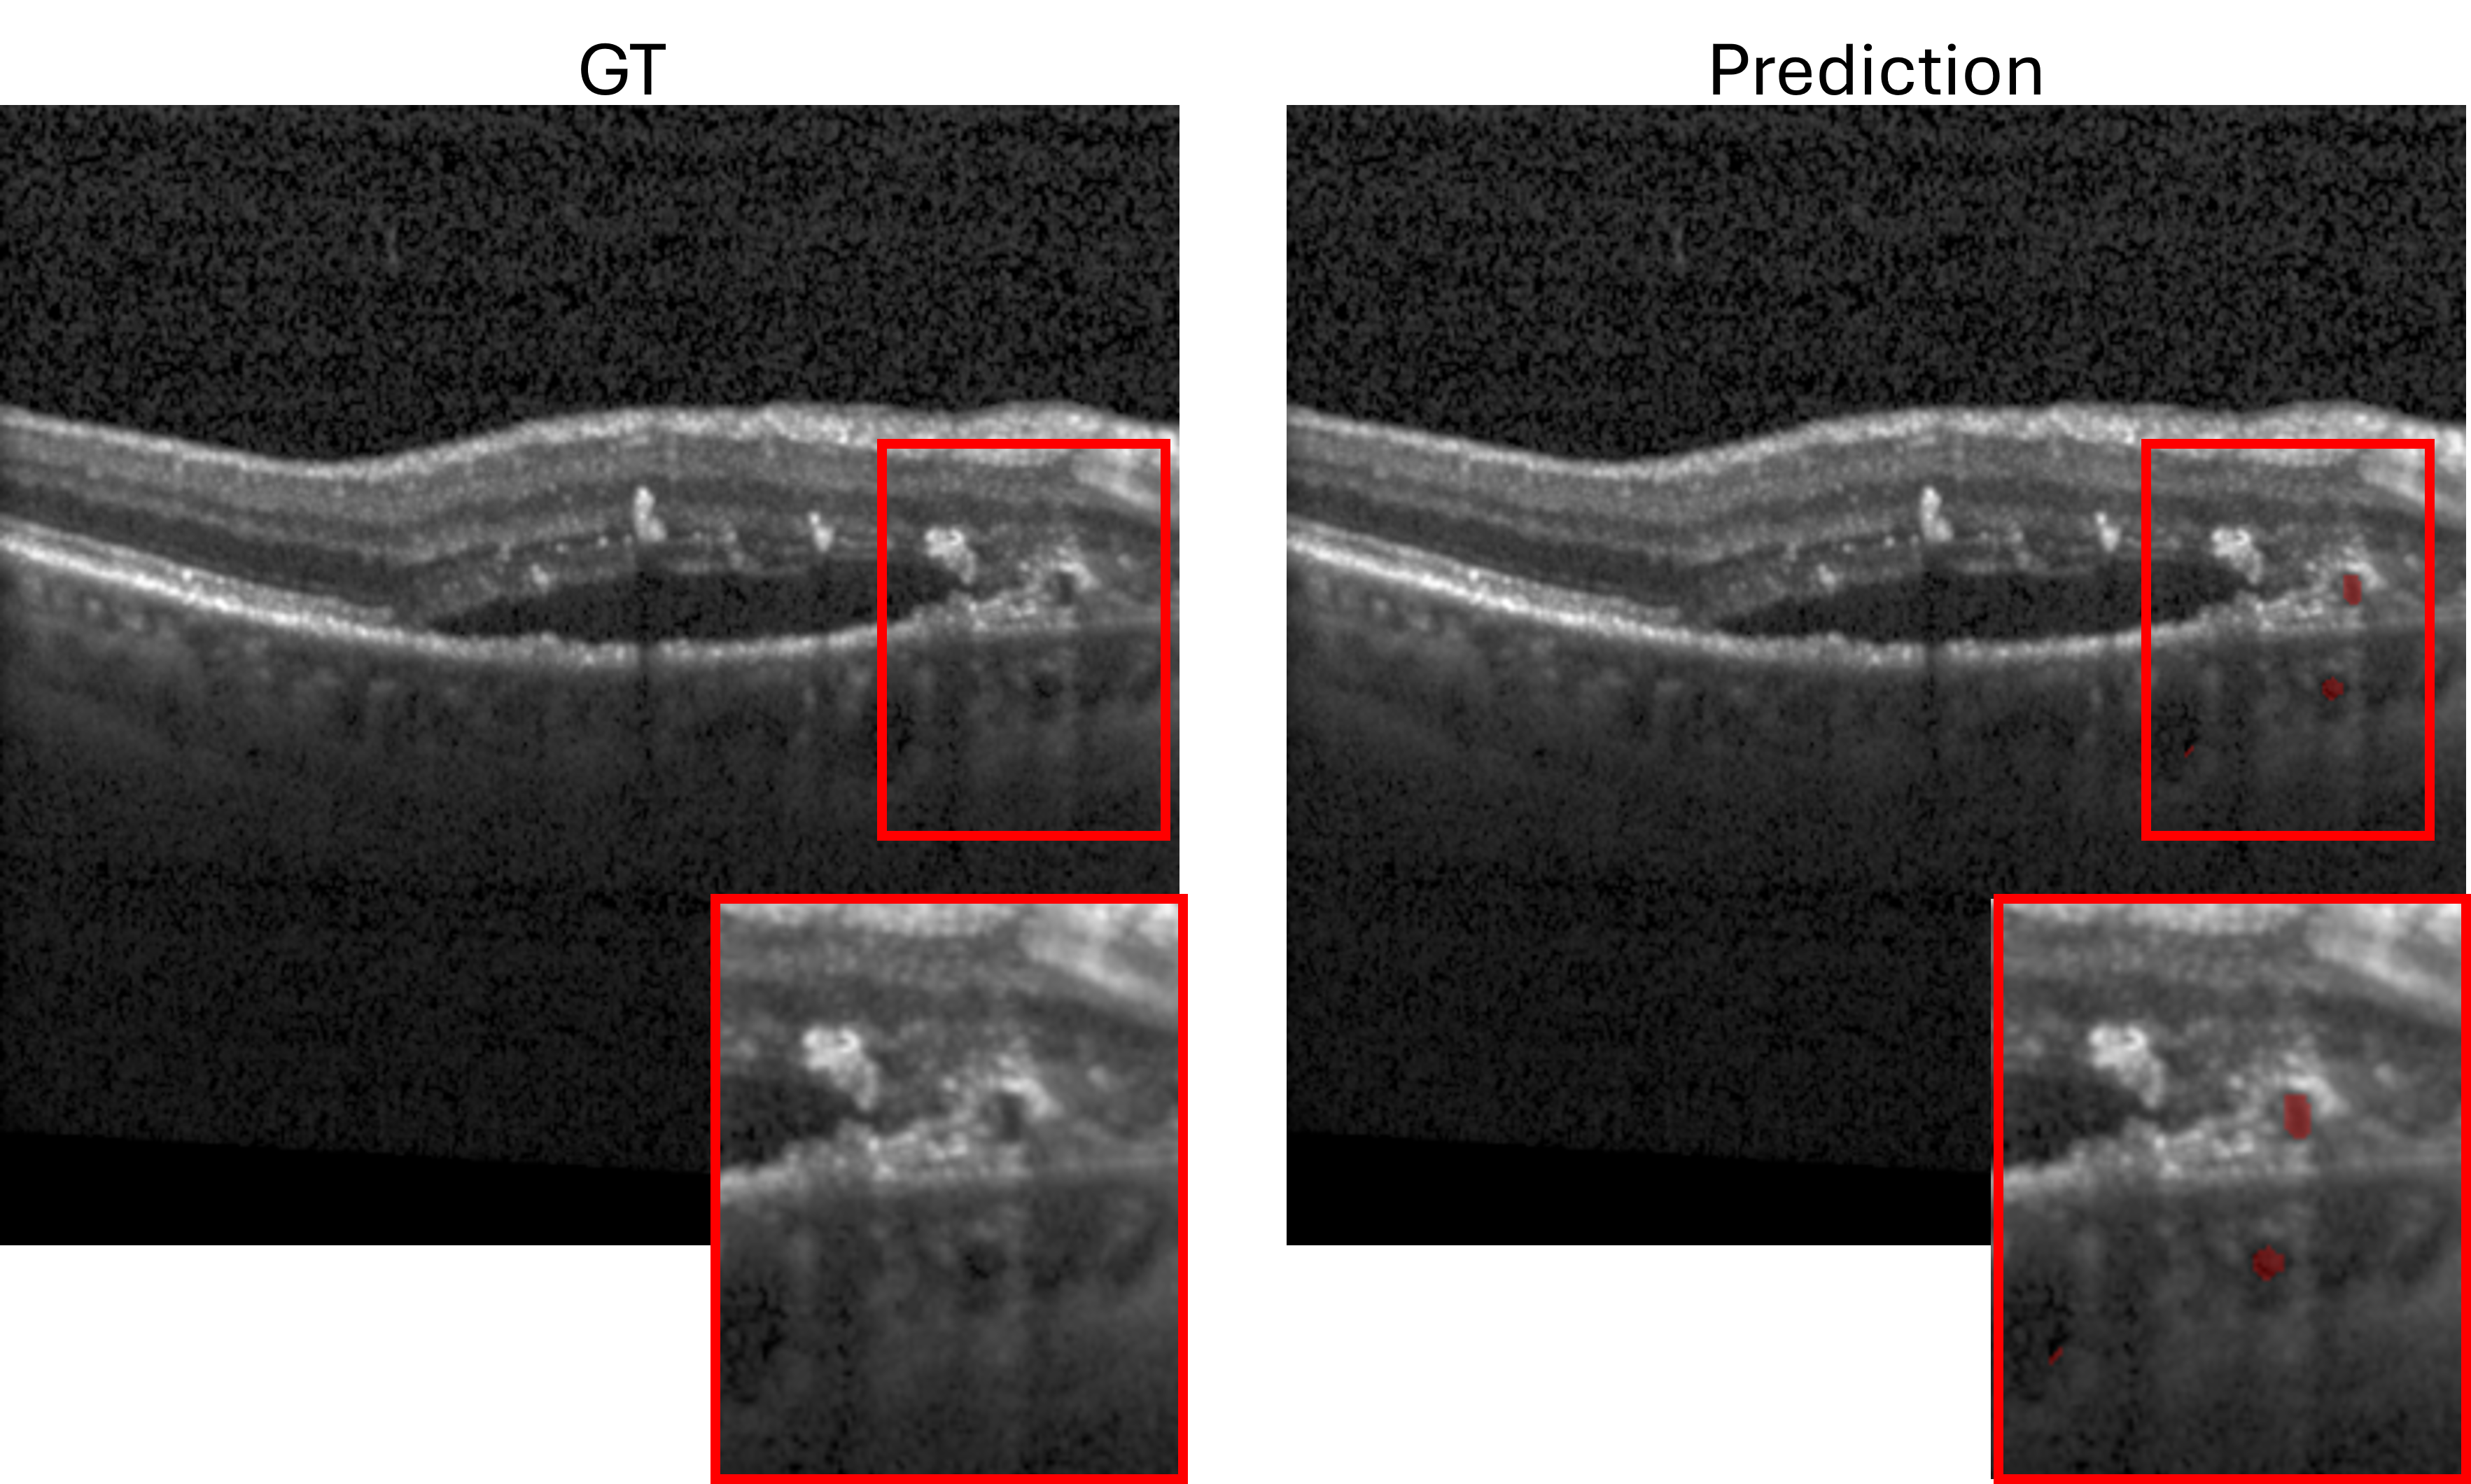
\includegraphics[width=0.8\linewidth]{figures/BCESegmentationError.png}
	\caption{Small oversegmentation performed in a Spectralis B-scan. This type of predictions appear commonly across multiple B-scans.}
	\label{fig:BCESegmentationError}
\end{figure}

\begin{figure}[!ht]
	\centering
	\includegraphics[width=0.8\linewidth]{figures/BCESegmentationDecent.png}
	\caption{Cirrus IRF segmentation performed by a model trained using BCE shown on the right, compared to its GT on the left. While this example has a decent segmentation, significant oversegmentation is seen on the top left of the image.}
	\label{fig:BCESegmentationDecent}
\end{figure}

\subsection{Experiment 1 and Experiment 2 Comparison in RETOUCH Dataset}

In order to compare Experiment 1 with Experiment 2, both their performances were presented in Table \ref{tab:Experiment1VsExperiment2}. These experiments are compared by evaluating each experiment's performance on the reserved fold. In the table, the first block corresponds to the performance obtained with the selected multi-class segmentation model, while the second block shows the performance of the combination of models from Experiment 2, with their masks combined in a probability-based approach.

\begin{table*}[!ht]
	\caption{Dice scores for every vendor and fluid in the reserved fold (fold 1), using the best models from Experiment 1 and Experiment 2. In Experiment 1, the model trained on Run 32 was selected, while in Experiment 2 the chosen models were those from Runs 42, for IRF, 52, for SRF, and 59, for PED. The rows with the same name must be compared with each other.}
	\centering
	\resizebox{\textwidth}{!}{\begin{tabular}{|c|c|c|ccc|ccc|ccc|c|c|c|c|}
			\hline
			% Headers
			\multirow{2}{*}{\textbf{Runs}} &
			\multirow{2}{*}{\textbf{Slices}} &  
			\multirow{2}{*}{\textbf{VF}} & 
			\multicolumn{3}{c|}{\textbf{Cirrus}} & 
			\multicolumn{3}{c|}{\textbf{Spectralis}} & 
			\multicolumn{3}{c|}{\textbf{Topcon}} & 
			\multicolumn{1}{c|}{\multirow{2}{*}{\textbf{IRF}}} & 
			\multirow{2}{*}{\textbf{SRF}} & 
			\multirow{2}{*}{\textbf{PED}} & 
			\multirow{2}{*}{\textbf{Fluid}} \\ \cline{4-12} & & &
			\multicolumn{1}{c}{\textbf{IRF}} & 
			\multicolumn{1}{c}{\textbf{SRF}} & 
			\textbf{\textbf{PED}} & 
			\multicolumn{1}{c}{\textbf{IRF}} & 
			\multicolumn{1}{c}{\textbf{SRF}} & 
			\textbf{PED} & 
			\textbf{IRF} & 
			\textbf{SRF} & 
			\textbf{PED} & 
			\multicolumn{1}{c|}{} & & & \\ 
			
			\hline

			\multirow{3}{*}{\textbf{Run 32}} & All & 1 & \multicolumn{1}{c|}{\textbf{0.852}} & \multicolumn{1}{c|}{\textbf{0.918}} & \textbf{0.934} & \multicolumn{1}{c|}{\textbf{0.645}} & \multicolumn{1}{c|}{\textbf{0.821}} & \textbf{0.852} & \multicolumn{1}{c|}{\textbf{0.818}} & \multicolumn{1}{c|}{\textbf{0.929}} & \textbf{0.755} & \textbf{0.799} & \textbf{0.905} & \textbf{0.841} & \textbf{0.742} \\
			
			& Fluid & 1 & \multicolumn{1}{c|}{0.654} & \multicolumn{1}{c|}{\textbf{0.799}} & \textbf{0.767} & \multicolumn{1}{c|}{0.645} & \multicolumn{1}{c|}{\textbf{0.687}} & \textbf{0.703} & \multicolumn{1}{c|}{0.624} & \multicolumn{1}{c|}{\textbf{0.744}} & \textbf{0.588} & 0.641 & \textbf{0.756} & \textbf{0.716} & \textbf{0.702} \\
			
			& No Fluid & 1 & \multicolumn{1}{c|}{\textbf{0.941}} & \multicolumn{1}{c|}{\textbf{0.972}} & \textbf{0.978} & \multicolumn{1}{c|}{\textbf{0.646}} & \multicolumn{1}{c|}{\textbf{0.889}} & \textbf{0.885} & \multicolumn{1}{c|}{\textbf{0.884}} & \multicolumn{1}{c|}{\textbf{0.960}} & \textbf{0.766} & \textbf{0.873} & \textbf{0.952} & \textbf{0.862} & \textbf{0.786} \\
			
			\hline
			\hline
			
			\multirow{3}{*}{\parbox{2cm}{\textbf{Runs 42, 52, and 59}}} & All & 1 & \multicolumn{1}{c|}{0.697} & \multicolumn{1}{c|}{0.787} & 0.428 & \multicolumn{1}{c|}{0.628} & \multicolumn{1}{c|}{0.631} & 0.178 & \multicolumn{1}{c|}{0.810} & \multicolumn{1}{c|}{0.864} & 0.531 & 0.733 & 0.792 & 0.427 & 0.544 \\
			
			& Fluid & 1 & \multicolumn{1}{c|}{\textbf{0.688}} & \multicolumn{1}{c|}{0.663} & 0.586 & \multicolumn{1}{c|}{\textbf{0.660}} & \multicolumn{1}{c|}{0.646} & 0.636 & \multicolumn{1}{c|}{\textbf{0.632}} & \multicolumn{1}{c|}{0.537} & 0.484 & \textbf{0.661} & 0.627 & 0.578 & 0.639 \\
			
			& No Fluid & 1 & \multicolumn{1}{c|}{0.701} & \multicolumn{1}{c|}{0.844} & 0.387 & \multicolumn{1}{c|}{0.520} & \multicolumn{1}{c|}{0.623} & 0.075 & \multicolumn{1}{c|}{0.870} & \multicolumn{1}{c|}{0.917} & 0.534 & 0.766 & 0.844 & 0.402 & 0.440 \\
			
			\hline
			
	\end{tabular}}
	\label{tab:Experiment1VsExperiment2}
\end{table*}

By looking at this table, the best segmentation performance becomes evident. The multi-class model consistently outperforms the binary models in across all fluids, vendors, and slice groups.
\par
Regarding the performances in fluids, the multi-class segmentation performs better than the binary models in all fluids when all the slices are considered and when only the slices which do not contain a certain fluid are considered. The only metrics in which the binary models outperform the multi-class is the segmentation of IRF in slices which contain this fluid. In these metrics, the binary models attain small improvements over the multi-class model. This fluid was also the one with the best performance in the set of slices with IRF, in Experiment 2.1. However, the segmentation of IRF in the slices which contain this fluid is not enough to compensate for the worse performance in fluid detection, when considering the slices without IRF. This was seen the major flaw of the binary segmentation models, which is tied to the models' weaker capability of understanding anatomical structures. This leads to a worse overall performance in IRF even when the segmentation is better. An example of similar performances between these models is seen in the IRF segmentations of Figures \ref{fig:Experiment2FinalModelPredictionsCirrus}, \ref{fig:Experiment2FinalModelPredictionsSpectralis}, and \ref{fig:Experiment2FinalModelPredictionsTopcon}.
\par
The performances reached by the binary model in SRF are worse than those obtained with the multi-class. While the predictions made with the binary model are still satisfactory, they are not as good as those made by the multi-class, as seen in the first case of the Figures \ref{fig:Experiment2FinalModelPredictionsCirrus} and \ref{fig:Experiment2FinalModelPredictionsTopcon}. This model shows a great detection of fluid, with a Dice coefficient greater than 0.85 in all classes, and the best fluid segmentation of all classes.
\par
The biggest performance difference between models are those observed in the PED class. The segmentation of PED in slices which contain this fluid is worse in the binary model than in multi-class. Despite the segmentation being worse across all vendors, the performance in the binary model is still acceptable. However, in the detection of fluid, the binary model performs poorly, especially when compared to the multi-class. These results are tied to the models' capabilities in identifying the region in which PED is located, which was seen to be much superior in multi-class. Two examples which show this are seen in the left side of Figure \ref{fig:Experiment2FinalModelPredictionsCirrus} and the segmentation in the bottom of Figure \ref{fig:Experiment2PEDSegmentation}, where the region segmented by PED does not occupy the entirety of the fluid, but only the section closest to its upper boundary.
\par
It is important to compare the results in the RETOUCH dataset with those obtained in the literature to better understand the impact and effect of the chosen methodology. \textcite{Alsaih2020} present an insightful study on the performance of multiple networks, including the U-Net, in the RETOUCH dataset. This paper was chosen as a benchmark for comparison due to the used dataset and the similarity with the selected methods. 
\par
In this article, the networks were trained and evaluated following a 3-fold approach, with the OCT volumes being equally distributed across the folds while still keeping a fair representation of vendors. The implementations in Experiment 1 and Experiment 2 were compared to two other base U-Net implementations in this paper: one trained with the entire image and another trained with patches. Multiple patch shapes (32 $\times$ 32, 64 $\times$ 64, 96 $\times$ 96, 128 $\times$ 128, 256 $\times$ 256, and 512 $\times$ 512) extracted with different overlapping percentages were tested, but the selected was 128 $\times$ 128 with 80\% overlapping as they obtained the best results. All the B-scans were previously resized to 572 $\times$ 572.
\par
For each model, \textcite{Alsaih2020} trained three networks with different optimizers: one using the stochastic gradient descent while the other two were trained using the Adam. Then, the results from each network were fused through majority voting. The results were also post-processed using a median filter.
\par
These differences bring advantages to the implementations by \textcite{Alsaih2020}, as they enhance the robustness and overall segmentation performance. While these changes provide a performance edge, it is challenging to find other studies with a comparable setup in terms of network architecture, dataset, and evaluation protocol. For these reasons, this paper was considered the most similar and, overall, suitable for comparison with the experiments presented here.
\par
In Table \ref{tab:Experiment1VsExperiment2VsLiterature}, the mean of the results in three validation folds of the models trained in \textcite{Alsaih2020} are shown, as well as the results from ``Set 7'' and ``Sets 10, 12, and 14'' together, representing the multiple binary models used in Experiment 2.

\begin{table*}[!ht]
	\caption{Dice scores for every fluid in ``Set 7'', ``Set 10, 12, and 14'', compared with the results obtained in the two networks by \textcite{Alsaih2020}.}
	\centering
	\begin{tabular}{|c|c|c|c|}
			\hline
			% Headers
			\textbf{Runs} & \textbf{IRF} & 
			\textbf{SRF} & 
			\textbf{PED} \\
						
			\hline
			
			\textbf{Set 7} & 0.67 & \textbf{0.80} & 0.72 \\
			
			\hline
			
			\textbf{Sets 10, 12, and 14} & 0.60 & 0.75 & 0.44 \\
			
			\hline
			\hline
			
			\textbf{U-Net \parencite{Alsaih2020}} & 0.29 & 0.47 & 0.18 \\
			
			\hline
			
			\textbf{U-Net with Patches \parencite{Alsaih2020}} & \textbf{0.68} & 0.61 & \textbf{0.84} \\
			
			\hline
			
	\end{tabular}
	\label{tab:Experiment1VsExperiment2VsLiterature}
\end{table*}

In this table, the first difference which presents a clear advantage in fluid segmentation is the use of patches as input. It becomes clear that the best segmentation performances in all fluids were achieved in the models which used patches. This enhances the model's capability of perceiving the image's finer details, which is deemed particularly helpful in IRF and PED.
\par
Despite the significant performance differences between the U-Net trained with the full image and the U-Net trained with patches implemented by \textcite{Alsaih2020}, the variation of performance in SRF is smaller than that seen in IRF and PED. This is because the use of patch-based inputs particularly favors the segmentation of localized fluids like IRF and PED, but not so much the SRF, since it depends on model capability to capture broader anatomical context. Since the SRF is often visually similar to the background, the patch-based approaches are more prone to misclassify it.
\par 
The use of vertical patches in Experiment 1 and 2 provides the anatomical context necessary for the segmentation of SRF, as reflected in the significantly better performance to that reported by \textcite{Alsaih2020}. In IRF segmentation, the difference in Dice scores between the two approaches is less pronounced. While the smaller patches used by \textcite{Alsaih2020} allow the model to focus on finer details, such as pixel intensity in fluid regions, the vertical patches from Experiment 1 and 2 offer a broader field of view that captures the structural references helpful for segmentation.
\par
For PED, the difference between experiments is also significant, though smaller than in SRF. However, the trend seen in this fluid is reversed to the one in SRF, as the models trained on smaller patches tend to perform better for PED. While models trained with vertical patches are more effective at determining the boundaries of PED fluid, they often lack the attention to the finer details. This is particularly relevant in cases with large PED regions, where the significant deformation of the retina causes parts of the fluid being positioned further away from key anatomical landmarks like the retinal layers. In such scenarios, models trained on smaller patches, which are attentive to details such as pixel intensity and less dependent on anatomical context, perform better. This contributes to the overall improved performance of models trained with smaller patches in segmenting PED.
\par
Overall, the models trained in Experiments 1 and 2 perform comparably or better than the U-Nets implemented by \textcite{Alsaih2020}, despite relying on a single network per task (one for multi-class segmentation in ``Set 7'' and one for binary segmentation in ``Sets 10, 12, and 14'') and excluding any post-processing steps. This highlights the effectiveness of the patch shape explored in these experiments, where it is both capable of capturing details fine enough to segment IRF, but also large enough to detect SRF. The absence of ensemble networks used for the same task or refinement techniques further emphasizes the robustness of the proposed approach, making it competitive and more efficient alternative for multi-class fluid segmentation in retinal OCT images.
\par
In a previous work, the authors also implemented the network developed by \textcite{Tennakoon2018}, using the same dataset. This network is a 2.5D segmentation network which receives three consecutive B-scans and segments the intermediate one. This model was trained in patches of shape 256 $\times$ 128, as done in Experiment 1.1 and the results from this model are shown in Table \ref{tab:Experiment1VsExperiment2VsTennakoon}. The implementation exhibited in this table corresponds to a single model performance, which was trained for 100 epochs using a 80\% training and 20\% testing split. A fair vendor representation was ensured in the split, but the quantities of fluid were not considered.

\begin{table*}[!ht]
	\caption{Dice scores for every vendor and fluid in Set 7, Set 10, 12, and 14, compared with the results obtained in the authors' previous implementation of the work by \textcite{Tennakoon2018}.}
	\centering
	\begin{tabular}{|c|c|c|c|c|}
		\hline
		% Headers
		\textbf{Runs} & \textbf{IRF} & 
		\textbf{SRF} & 
		\textbf{PED} &
		\textbf{Fluid} \\
		
		\hline
		
		\textbf{Set 7} & 0.67 & 0.80 & \textbf{0.72} & \textbf{0.63} \\
		
		\hline
		
		\textbf{Sets 10, 12, and 14} & 0.60 & 0.75 & 0.44 & - \\
		
		\hline
		\hline
		
		\textbf{\textcite{Tennakoon2018} Implementation} & \textbf{0.71} & \textbf{0.85} & 0.71 & 0.62 \\
		
		\hline
		
	\end{tabular}
	\label{tab:Experiment1VsExperiment2VsTennakoon}
\end{table*}

In this table, it is seen that the 2.5D implementation performs better than the models in ``Set 7'' and ``Sets 10, 12, and 14'' in IRF and SRF, but worse in PED and in overall fluid.
\par
The main advantage when using this model is the use of the surrounding slices as a way to capture the context around the fluid regions. The small transitions, which are noticeable when seeing three consecutive slices, allow the model to learn the limiting regions of the fluids. This understanding of surrounding areas, combined with the attention to small changes motivated by the training in small patches, makes this model capable of both fine and coarse segmentation, as it is able to know the limits of fluid regions independently of their size. 
\par
This explains the improved segmentation of SRF, as the model better captures the small transitions in the SRF regions while still understanding the changes in the space around it which allow for the identification of this fluid. Similarly, the small patches also promote a better segmentation of IRF, where the understanding of small transitions is required for a correct segmentation.
\par
In PED, the performance is worse, but mainly due to the conditions in which this model was trained. Since the data was split randomly, the training volumes contained large quantities of PED, which led to the prediction of significant quantities of this fluid in multiple B-scans. For this reason, the Dice coefficient when considering all the fluid as binary was also deeply penalized, as seen in the table. 
\par
However, it is important to note that the results shown do not come from a cross-validation, and instead of a single split. This means that not only the 2.5D segmentation model was trained on more data than the those in Experiment 1 and 2 (approximately 60\% of the RETOUCH dataset), it could also have a split which benefits or harms the models performance.

\subsection{Experiment 1 and Experiment 2 Comparison in CHUSJ Dataset}

The results obtained in the CHUSJ private dataset were not as good as those obtained in the \hbox{RETOUCH}, in which the model was trained. The main cause for this poor segmentation is difference between the RETOUCH and CHUSJ dataset regarding image quality and segmentation criteria. In Table \ref{tab:CHUSJSegmentationResults}, the Dice coefficients across multiple vendors and fluids are shown, both for the images in their original shape and resized to $496 \times 512$. Since the segmentation U-Net is a fully convolutional network and does not contain any shape-dependent layer, the trained models can be applied to dataset B-scans in their original shape or resized.

\begin{table*}[!ht]
	\caption{Dice scores for every vendor and fluid in the CHUSJ dataset, using the best models from Experiment 1 and Experiment 2.}
	\centering
	\begin{tabular}{|c|c|c|c|c|c|c|}
			\hline
			% Headers
			\textbf{Runs} &
			\textbf{Resized} &
			\textbf{Slices} &  
			\textbf{IRF} & 
			\textbf{SRF} & 
			\textbf{PED} & 
			\textbf{Fluid} \\
			
			\hline
			
			\multirow{3}{*}{\textbf{Run 32}} & \multirow{3}{*}{No} & All & 0.167 & 0.441 & \textbf{0.141} & \textbf{0.209} \\
			
			& & Fluid & \textbf{0.510} & \textbf{0.541} & 0.011 & \textbf{0.317} \\
			
			& & No Fluid & 0.142 & 0.380 & \textbf{0.143} & \textbf{0.125} \\
			
			\hline
			
			\multirow{3}{*}{\textbf{Run 32}} & \multirow{3}{*}{Yes} & 
			All & \textbf{0.191} & 0.455 & 0.132 & 0.176 \\
			
			& & 
			Fluid & 0.475 & 0.533 & 0.023 & 0.300 \\
			
			& & 
			No Fluid & \textbf{0.170} & 0.408 & 0.134 & 0.078 \\
			
			\hline
			\hline
			
			\multirow{3}{*}{\parbox{2cm}{\textbf{Runs 42, 52, and 59}}} & \multirow{3}{*}{No} & All & 0.046 & 0.498 & 0.001 & 0.079 \\
			
			& & 
			Fluid & 0.403 & 0.460 & \textbf{0.054} & 0.180 \\
			
			& & 
			No Fluid & 0.019 & 0.521 & 0.000 & 0.000\\
			
			\hline
			
			\multirow{3}{*}{\parbox{2cm}{\textbf{Runs 42, 52, and 59}}} & \multirow{3}{*}{Yes} & 
			All & 0.038 & \textbf{0.563} & 0.001 & 0.078 \\
			
			& & 
			Fluid & 0.412 & 0.468 & 0.040 & 0.178 \\
			
			& & 
			No Fluid & 0.009 & \textbf{0.620} & 0.000 & 0.000\\
			
			\hline
			
	\end{tabular}
	\label{tab:CHUSJSegmentationResults}
\end{table*}

In the RETOUCH dataset, the volumes were extracted with consistent dimensions and noise levels across the same vendor. This results in visually similar images, whose differences can be attributed to the patient's characteristics. Therefore, while the differences seen in the CHUSJ dataset are a good test to understand the models' robustness, those trained in RETOUCH did not generalize well to this new dataset, as the visually similar images seen in training do not prepare the model for images with different visual appearances. In Figure \ref{fig:CHUSJProblematicImages}, three B-scans with really different characteristics are shown. The left B-scan is well oriented, but the choroid region is very defined, as opposed to the RETOUCH images where this region is blurry. The middle and right B-scan present an odd orientation and are much noisier than the examples seen in training.

\begin{figure}[!ht]
	\centering
	\includegraphics[width=1.0\linewidth]{figures/CHUSJProblematicImages.png}
	\caption{Three B-scans with characteristics different from those in RETOUCH. The left scan shows definition on the choroid, while the middle and right scan present an odd orientation and significant noise.}
	\label{fig:CHUSJProblematicImages}
\end{figure}

The last problem when considering segmentation masks from different sources is the criteria used in the segmentation. In medical images, the segmentation performed by different professionals may result in different outcomes, as shown in Figure \ref{fig:RETOUCHSegmentationDifferences}. Therefore, the criteria followed to segment fluid by the evaluator on CHUSJ dataset may be different from the criteria followed in the RETOUCH dataset. Furthermore, considering that in RETOUCH the approach to merge predictions by different evaluators is to consider both correct, the models trained in this data are prone to oversegment in unseen volumes.
\par
An example of different segmentation criteria between the RETOUCH and CHUSJ datasets is seen in Figure \ref{fig:RETOUCHvsCHUSJSegmentationCriteria}, where visually and anatomically similar regions are segmented only in one dataset. While in manual segmentation the context from the surrounding slices is relevant, the visual similarity between regions is the most important characteristic in the segmentation using CNNs. Therefore, when visually similar regions are not segmented equally or following the same criteria in the training and testing data, the predicted segmentation masks for the testing volumes did not coincide with the GT.

\begin{figure}[!ht]
	\centering
	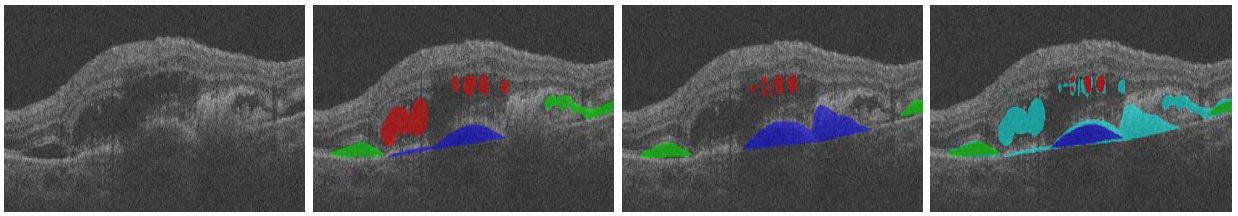
\includegraphics[width=1.0\linewidth]{figures/RETOUCHSegmentationDifferences.png}
	\caption{Significantly different segmentations (middle images) of the same B-scan (left image) by different evaluators, in the RETOUCH dataset. The mask seen in cyan in the last image represents the final fluid regions when considering both evaluations \parencite{Bogunovic2019b}.}
	\label{fig:RETOUCHSegmentationDifferences}
\end{figure}

\begin{figure}[!ht]
	\centering
	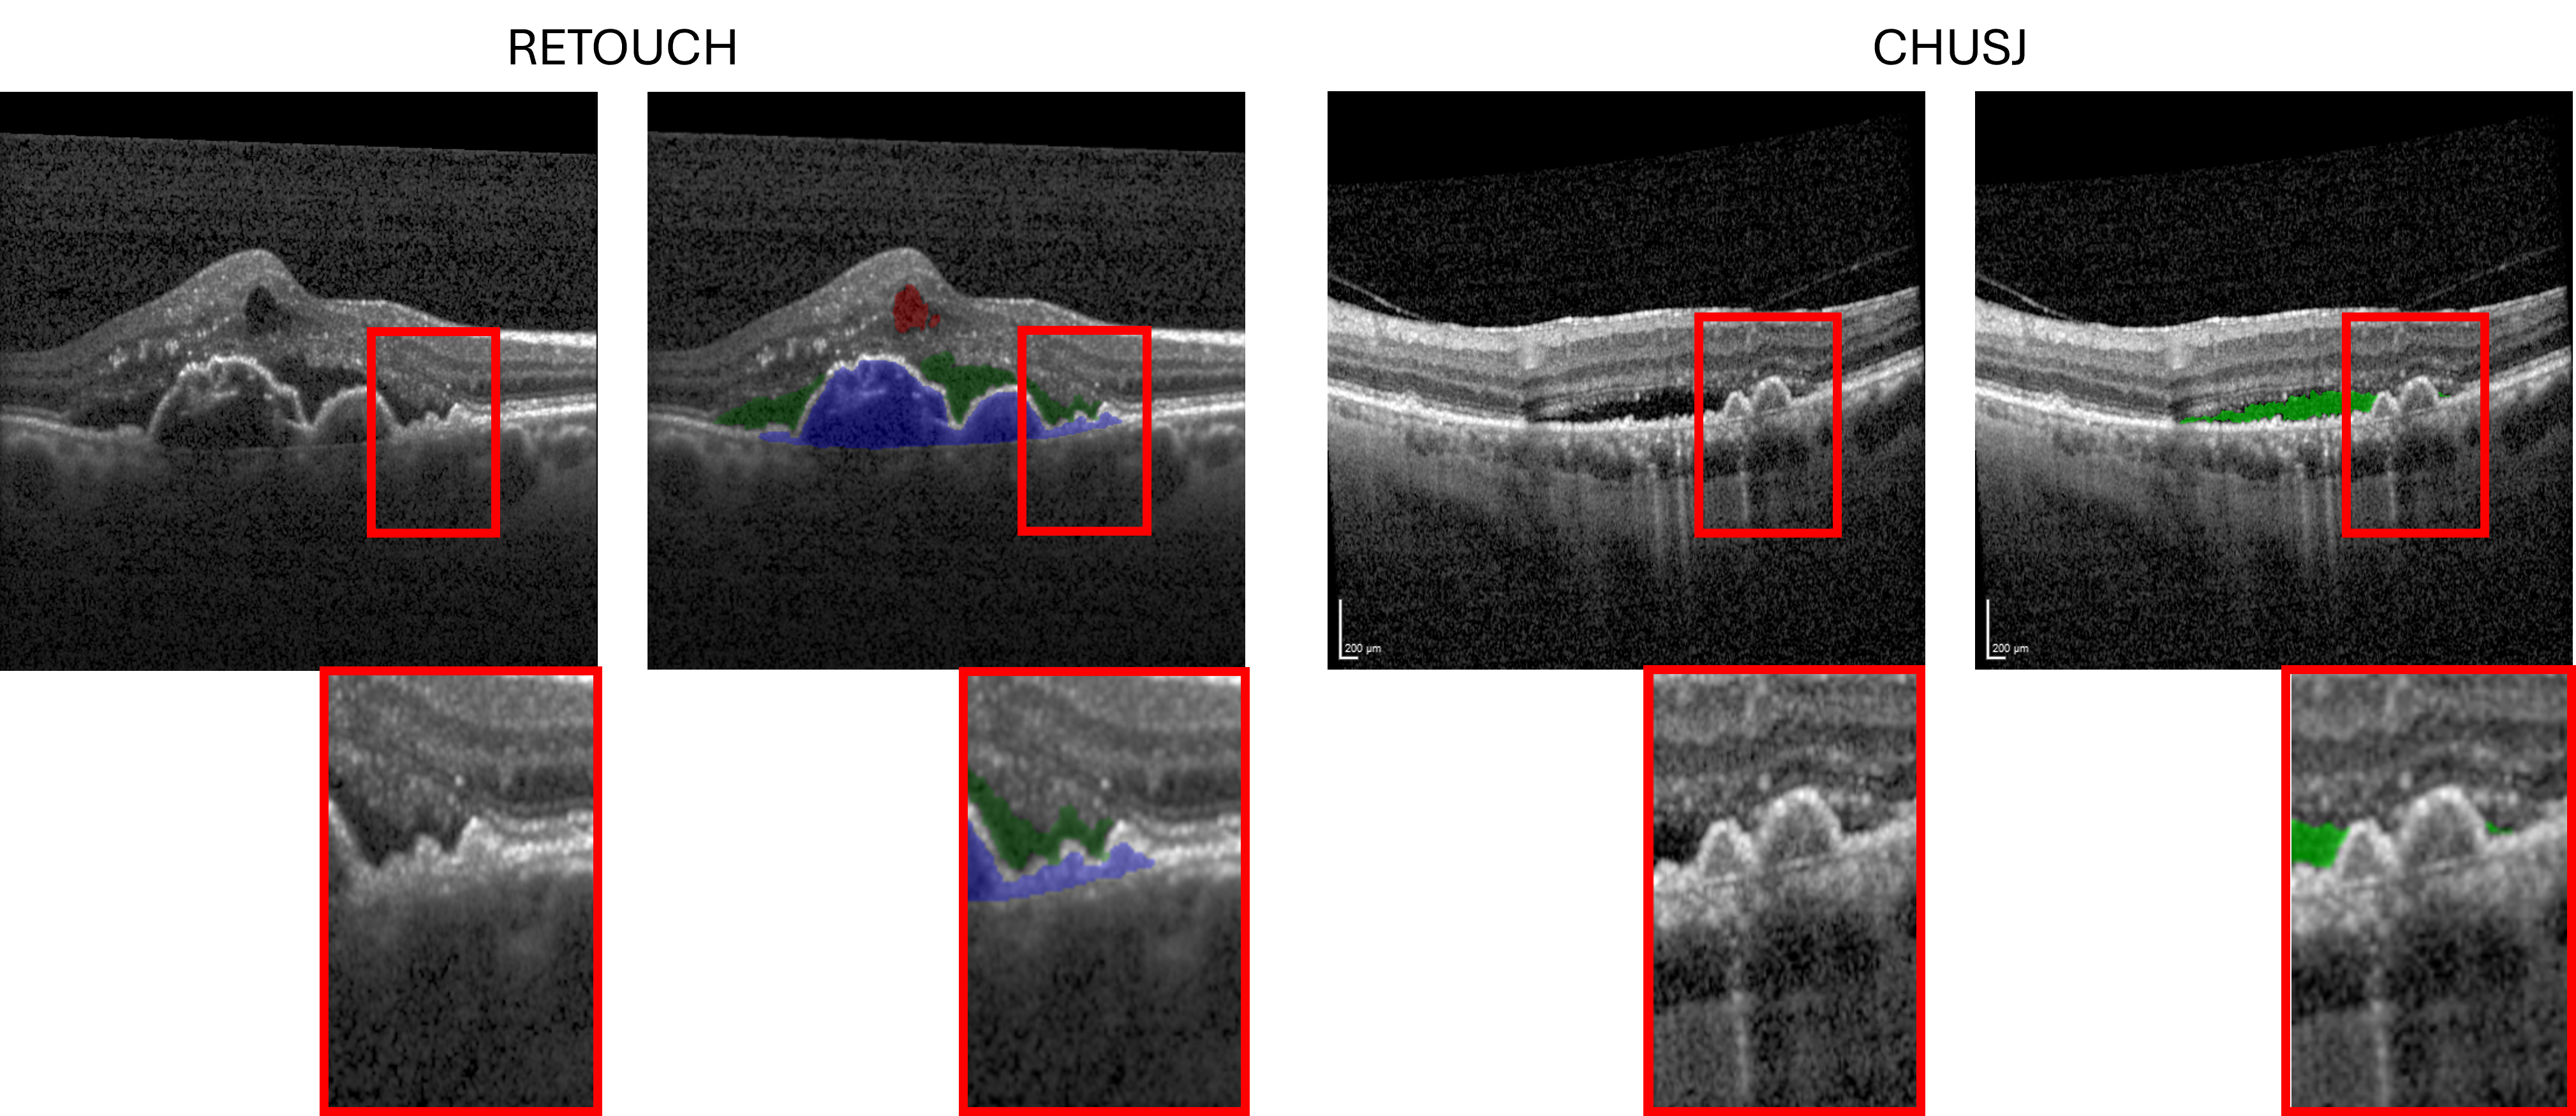
\includegraphics[width=1.0\linewidth]{figures/RETOUCHvsCHUSJSegmentationCriteria.png}
	\caption{Visually similar PED regions are segmented in one dataset but not on the other. This ambiguous segmentation can translate to worse performances in the model testing.}
	\label{fig:RETOUCHvsCHUSJSegmentationCriteria}
\end{figure}

The worst performing fluid segmented in this dataset is the PED. In the binary models, this fluid was wrongfully detected in every slice. The oversegmentation and prediction of PED was already a problem seen in previous experiment, especially in the Spectralis volumes during Experiment 2. The segmentation in slices with PED also resulted in small Dice coefficients. While this is largely due to the oversegmentations across multiple slices, it is also impacted by the small quantity of PED present across the entire dataset. However, it is important to note that many of the oversegmentations are in regions where the presence of PED could vary according to the applied segmentation criteria. In Figure \ref{fig:CHUSJPEDSegmentation}, two slices and their respective GT are shown, highlighting the segmentation of PED in a region which could be segmented with this fluid and a satisfying segmentation of SRF.

\begin{figure}[!ht]
	\centering
	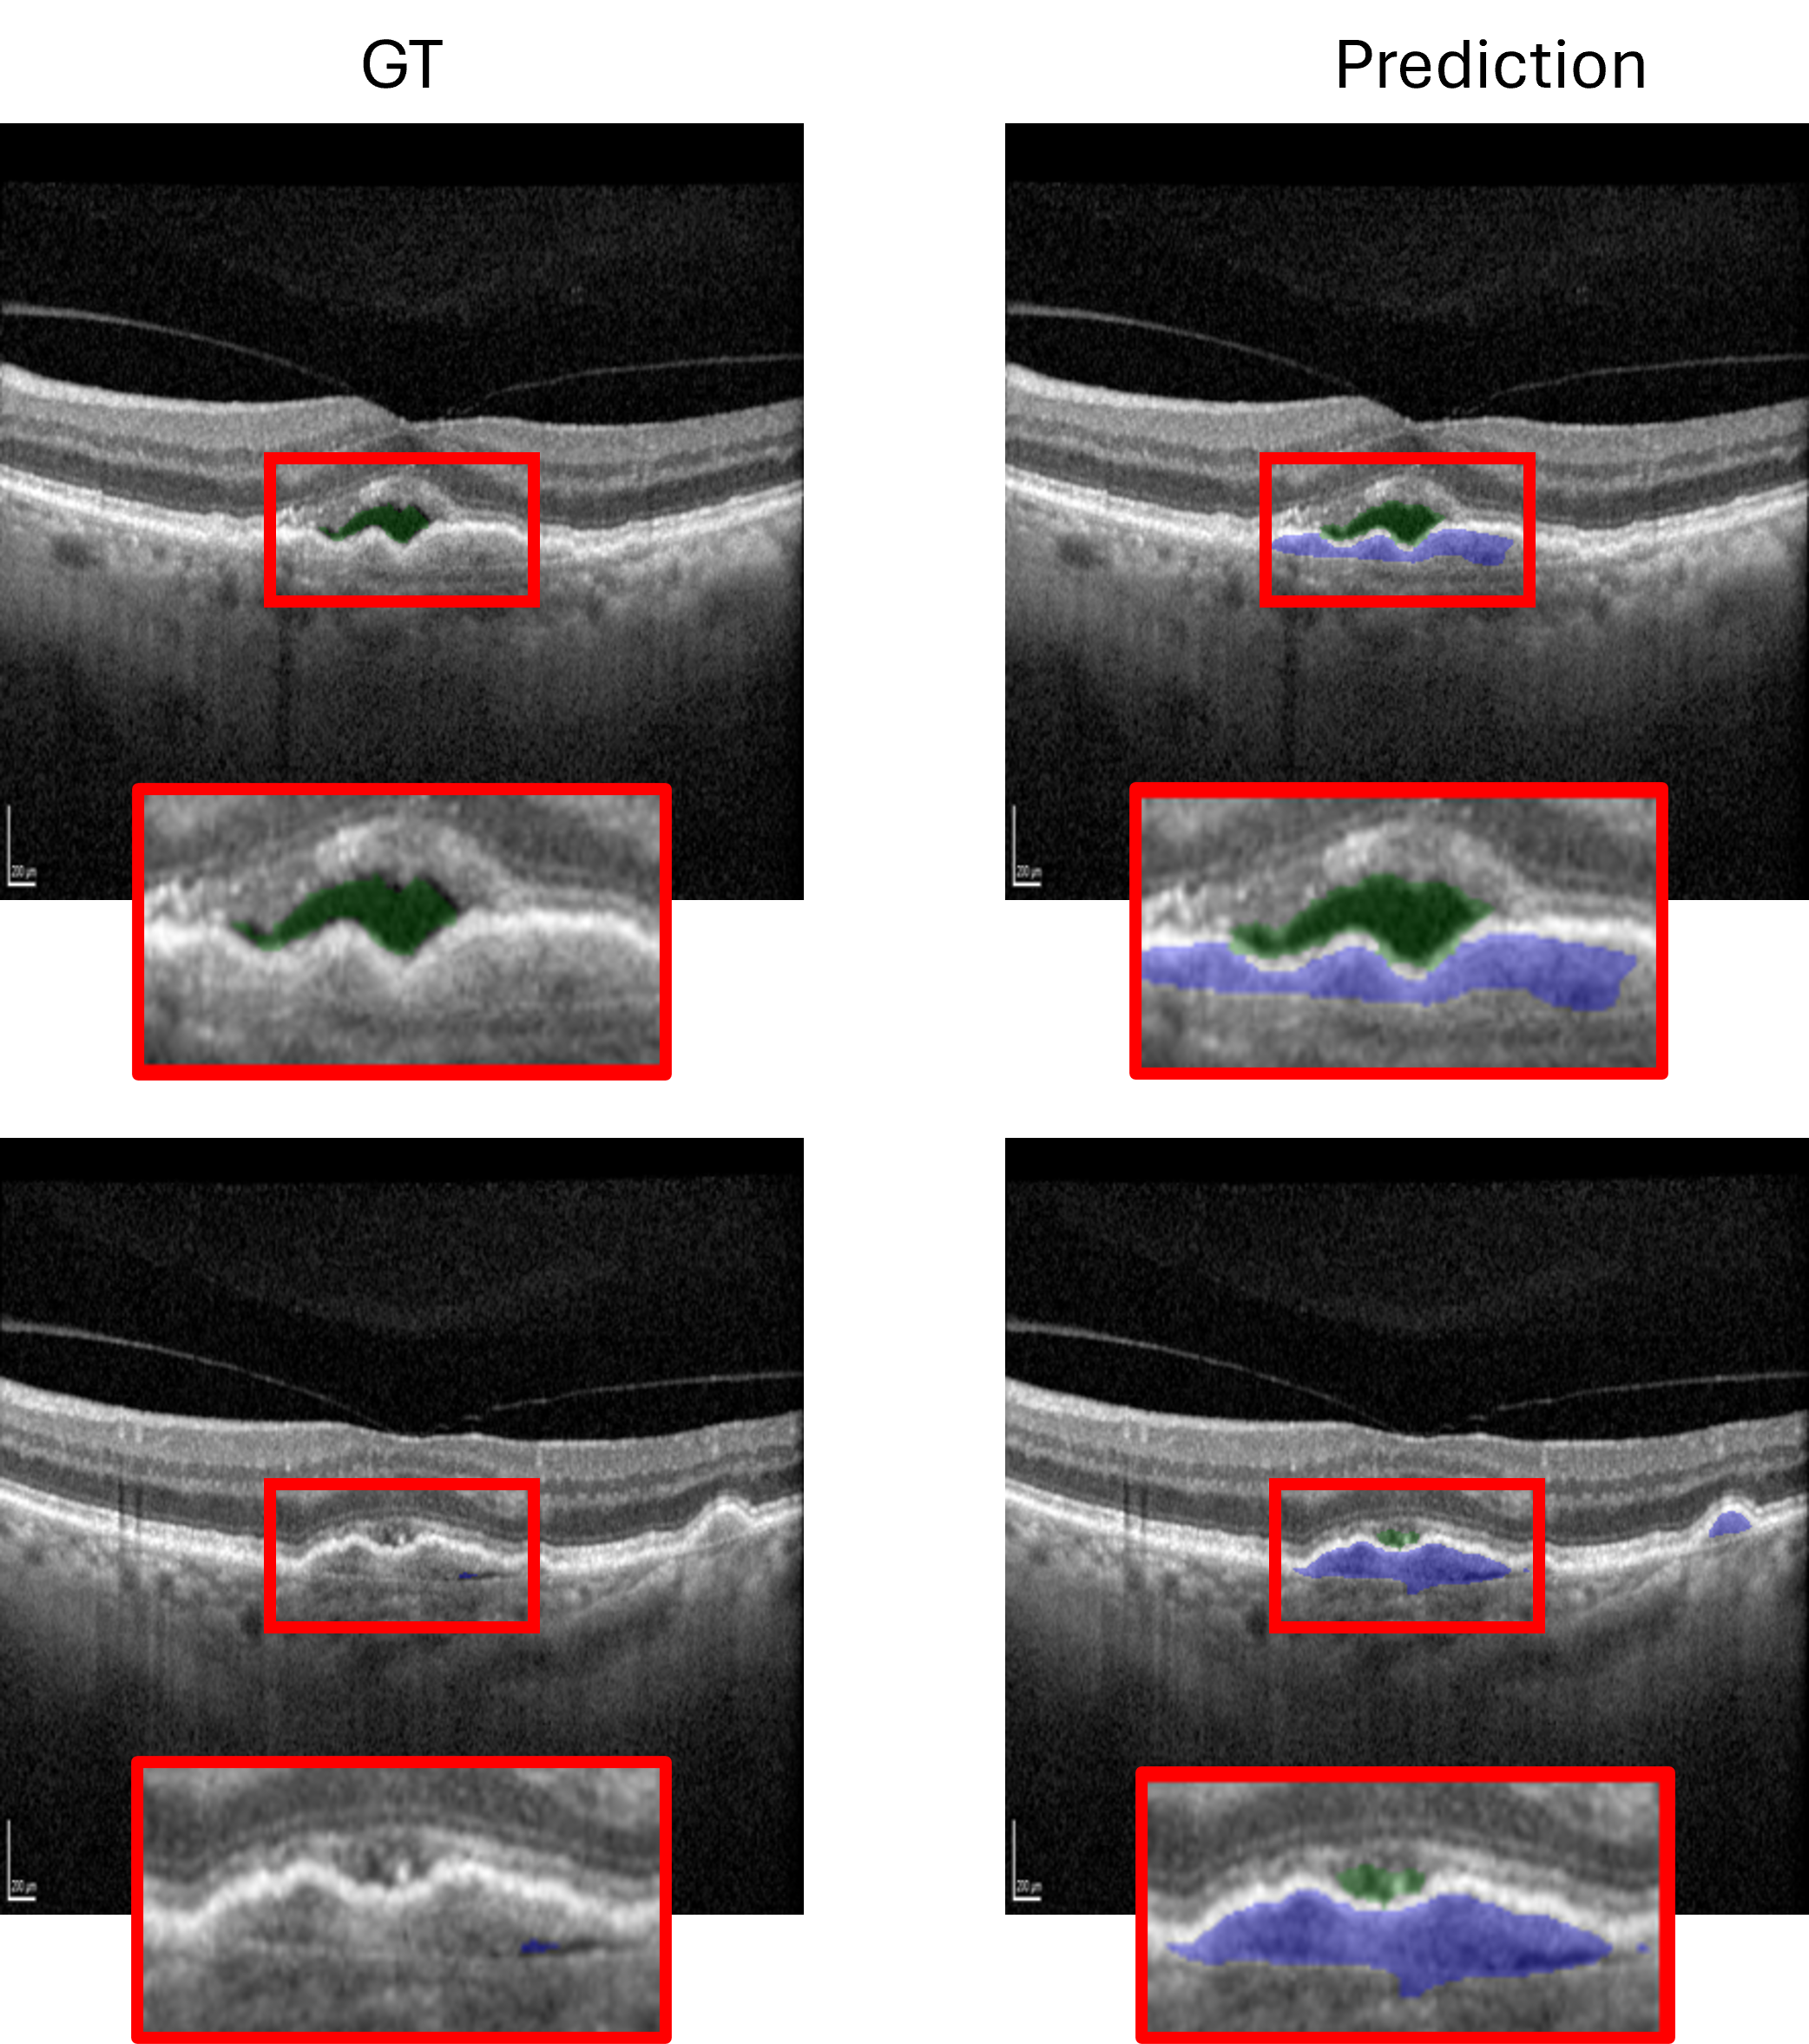
\includegraphics[width=0.65\linewidth]{figures/CHUSJPEDSegmentation.png}
	\caption{SRF and PED segmentation in two B-scans from CHUSJ. The regions segmented by the model as PED could also be considered fluid, depending on the criteria applied.}
	\label{fig:CHUSJPEDSegmentation}
\end{figure}

The segmentation of SRF was the most consistent in this dataset. While the Dice coefficients are smaller than those obtained in the RETOUCH dataset, a worse performance was expected in the CHUSJ, highlighted by its diversity of images and different criteria than those applied in RETOUCH. In Figure \ref{fig:CHUSJSRFSegmentation}, the segmentation of a B-scan with SRF is shown. While the segmentation by the model correctly identifies the SRF region, a slight oversegmentation is performed. This is seen across multiple B-scans, influenced by the data in which it was trained, resulting in a worse Dice score in the slices with fluid.

\begin{figure}[!ht]
	\centering
	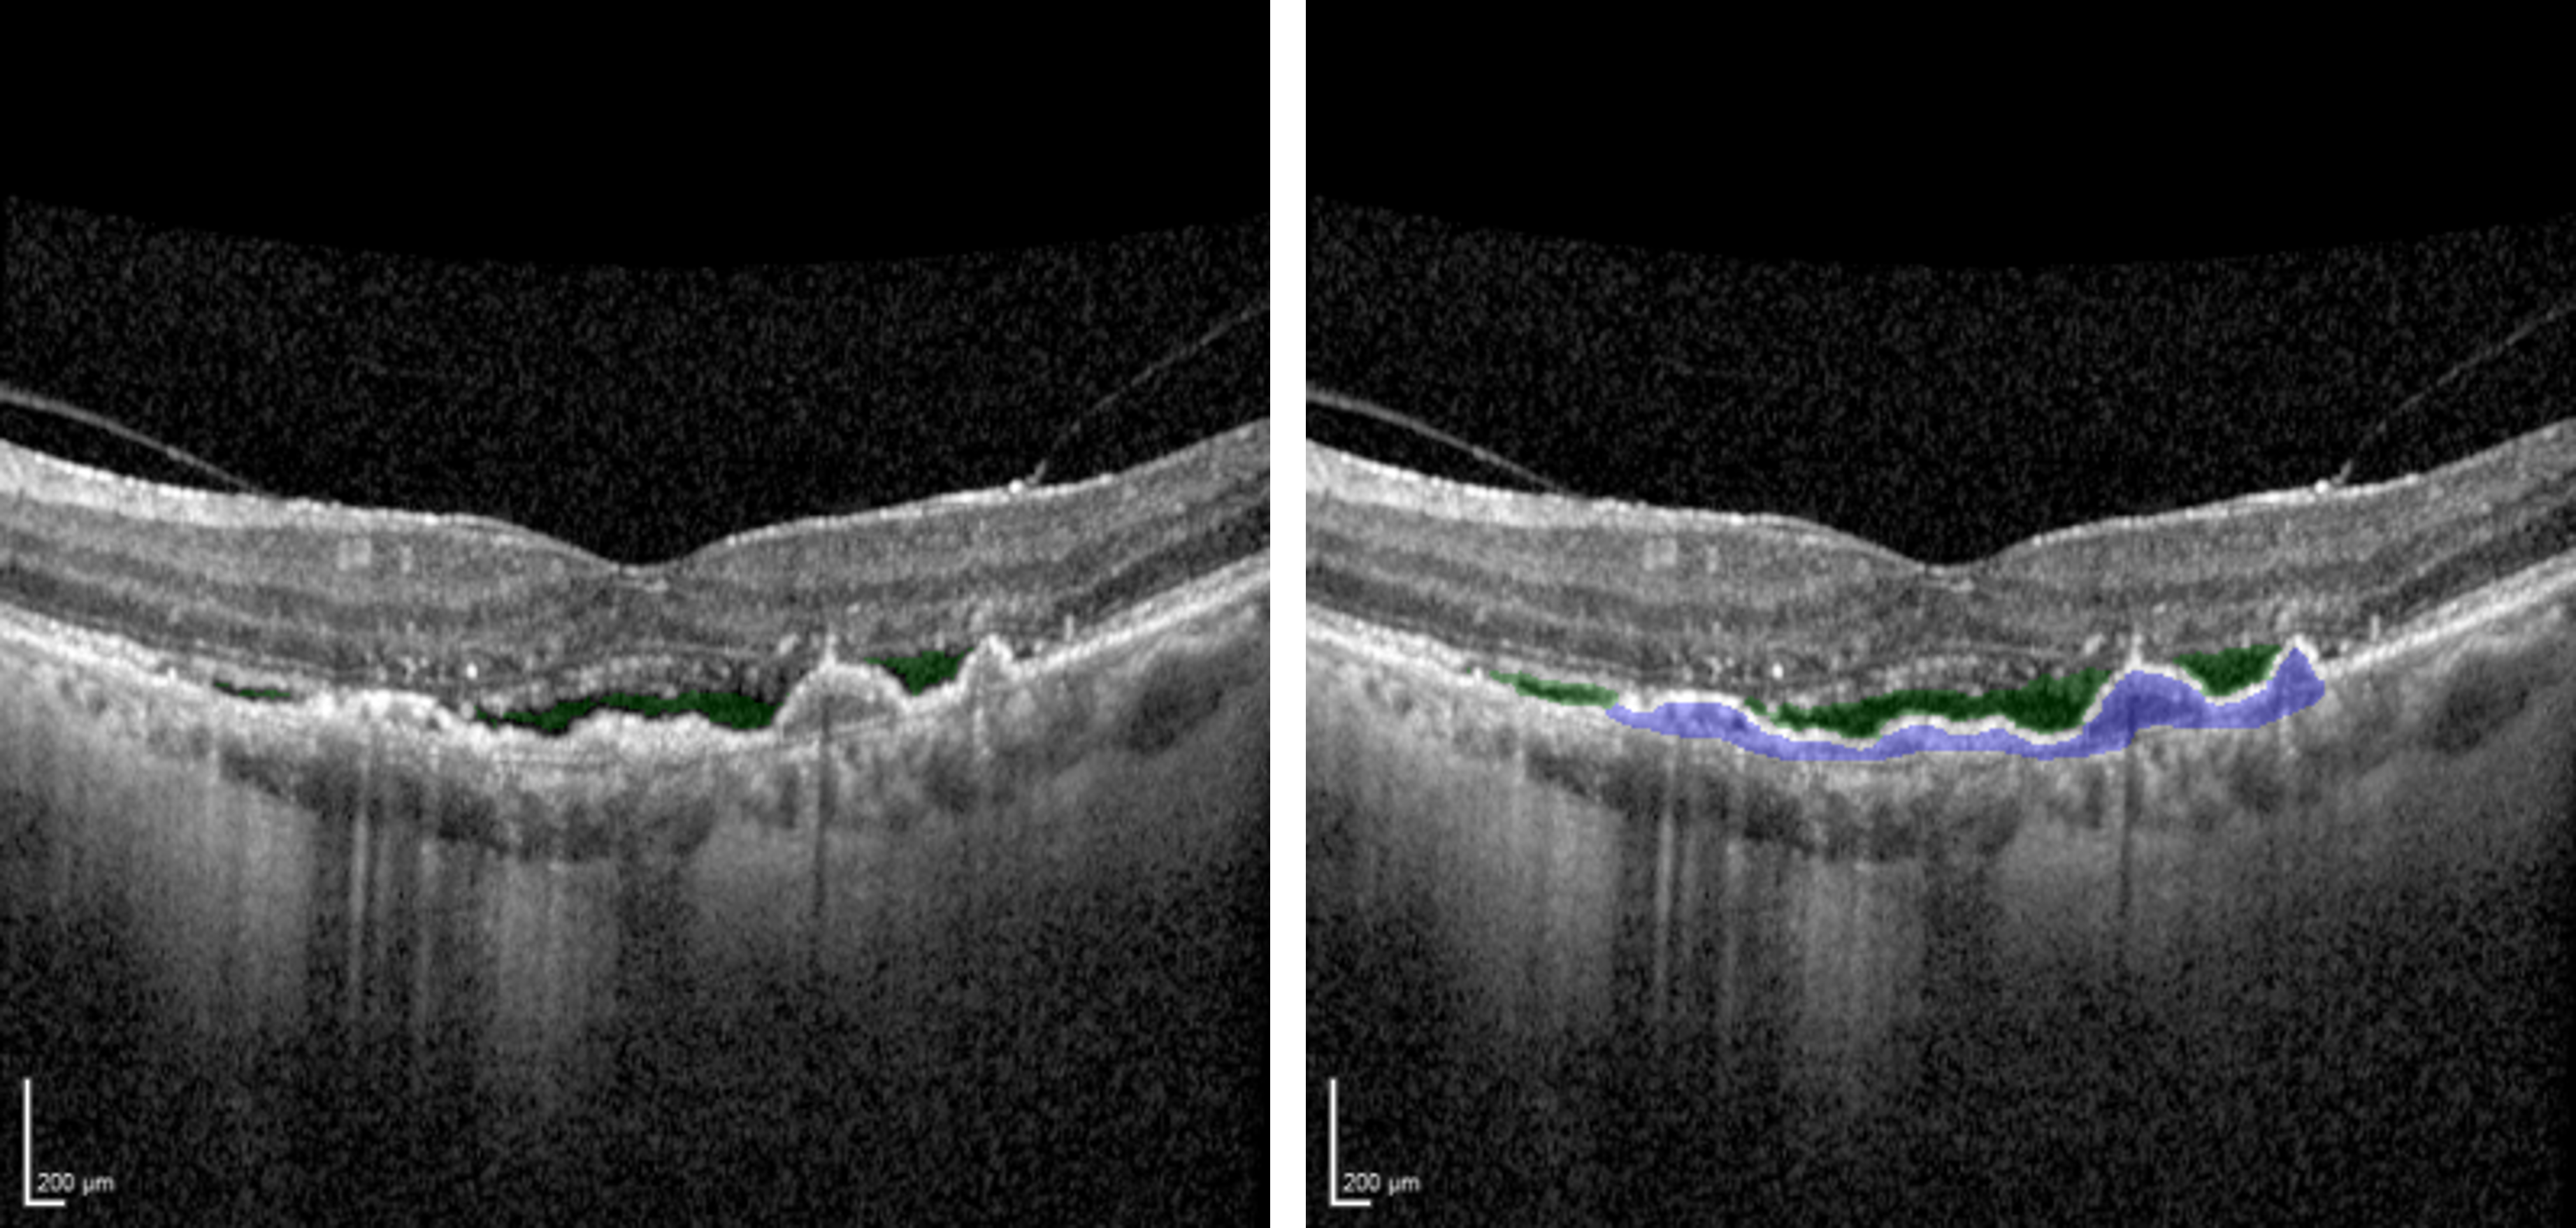
\includegraphics[width=0.60\linewidth]{figures/CHUSJSRFSegmentation.png}
	\caption{SRF and PED segmentation (right) in a B-scan from CHUSJ, compared to its GT (left). This shows the tendency to oversegmentation by the model.}
	\label{fig:CHUSJSRFSegmentation}
\end{figure}

Similar to SRF, the IRF segmentation is also decent in the slices which contain this fluid. Likewise, the model tends to slightly oversegment the fluid regions, as seen in Figure \ref{fig:CHUSJIRFSegmentation}. 

\begin{figure}[!ht]
	\centering
	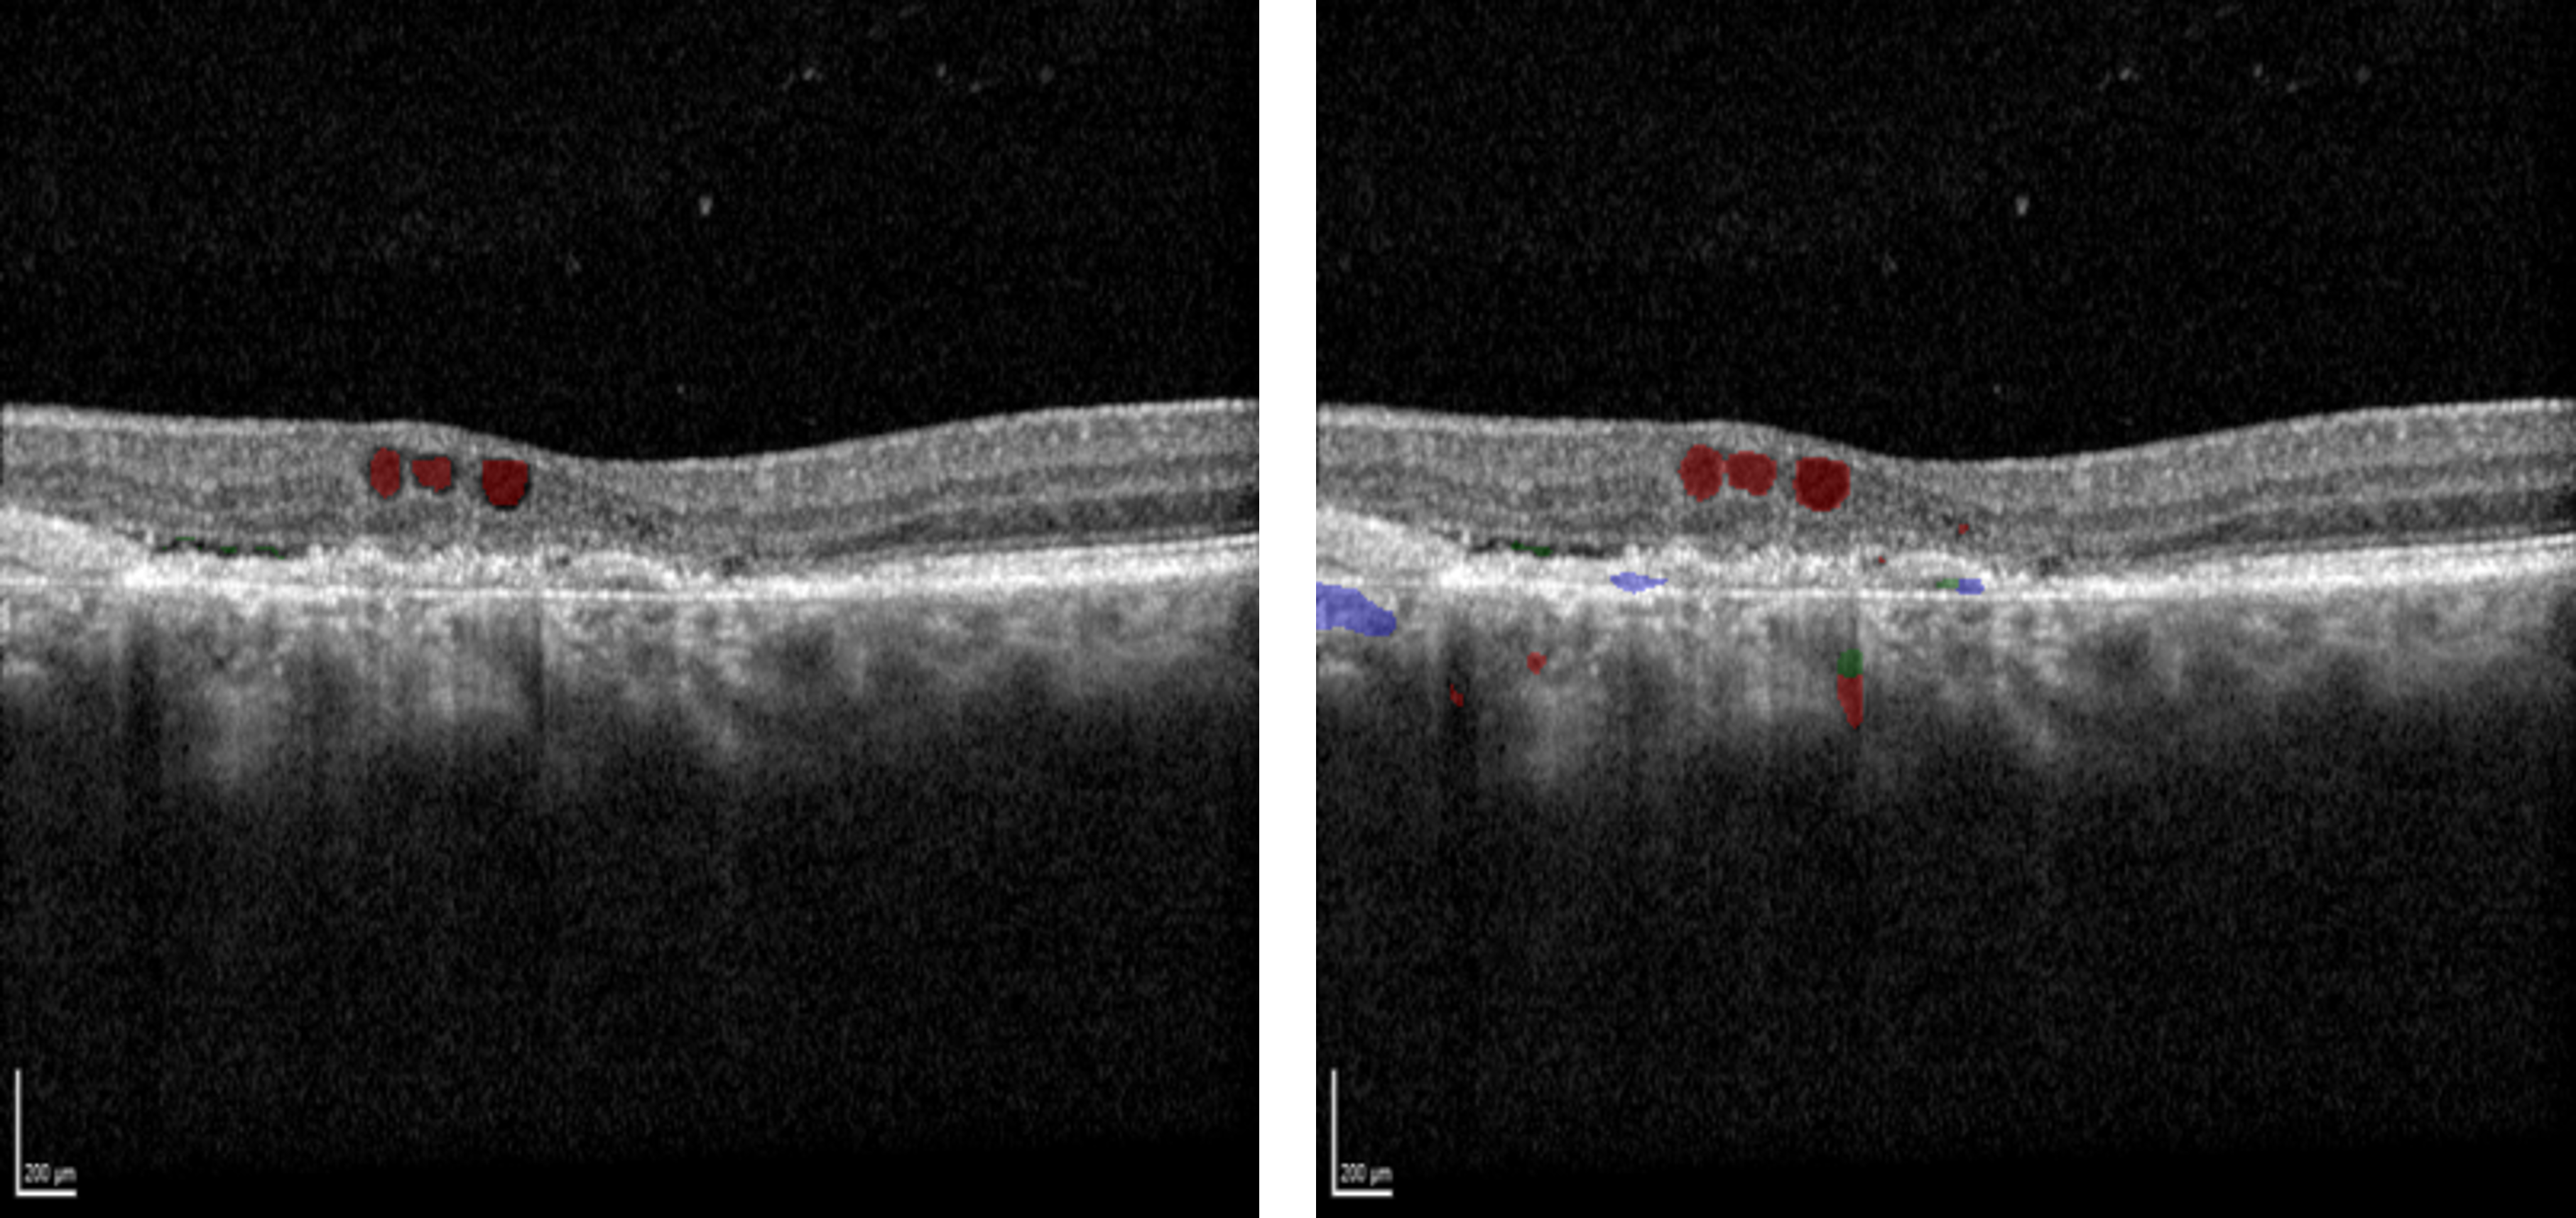
\includegraphics[width=0.60\linewidth]{figures/CHUSJIRFSegmentation.png}
	\caption{Segmentation of IRF regions (right) compared to its respective GT (left). The prediction of fluid regions in the choroid is also noticeable.}
	\label{fig:CHUSJIRFSegmentation}
\end{figure}

However, the main reason behind the poor Dice coefficients when considering all the slices is the fluid detection. In slices in which the fluids are not present, particularly in IRF and PED, they are still predicted outside the retina, usually in the choroid. While this is already visible in Figure \ref{fig:CHUSJIRFSegmentation}, where all the fluids are segmented in the choroid, more examples are shown in Figure \ref{fig:CHUSJChoroidSegmentation}.

\begin{figure}[!ht]
	\centering	\includegraphics[width=0.65\linewidth]{figures/CHUSJChoroidSegmentation.png}
	\caption{Segmentation of multiple fluids in the choroid region of the B-scans. This is performed often, significantly reducing the Dice coefficients seen in Table \ref{tab:CHUSJSegmentationResults}.}
	\label{fig:CHUSJChoroidSegmentation}
\end{figure}

The incorrect segmentations in the choroid are caused by the different quality of the image in this dataset, previously explained. When training the segmentation models with the RETOUCH dataset, the Spectralis scans are focused on the retinal layers, blurring the structures outside of it, including the choroid. In the B-scans which compose the CHUSJ dataset, this region is not blurred. This confuses the segmentation model which also interpret the choroid as retina, thus predicting the existence of fluid regions there. The fluid which is the most affected by this segmentation is the IRF, due to the resemblance with the structures and intensities present in this region. Therefore, in case the region outside the retina was not considered in the final masks, the Dice coefficients would improve significantly. These segmentation errors are more prominent in the predictions performed by the binary models' segmentation as they present weaker capabilities of understanding anatomic references, basing their predictions more on the pixels intensities, thus being more easily fooled by the choroid.
\par
The use of resized images or their original shape did not translate to a significant difference in segmentation, as the performances remained almost unchanged when varying the slices shape. Since these transformations are applied along the horizontal axis, the different resolutions are harder to perceive, as they do not significantly change the perception of the structures in the B-scan.
\par
Lastly, the influence of the noise and different perceptions present in this dataset, as in the examples shown in Figure \ref{fig:CHUSJProblematicImages}, is more significant outside the retina. In Figure \ref{fig:CHUSJSegmentationOnNoisyScans}, the segmentation of these noisy B-scans is shown, where a decent segmentation of SRF is seen, with a prediction of PED coherent with the training data. However, it is outside the retina, in the choroid, where the wrong IRF segmentations are seen.

\begin{figure}[!ht]
	\centering	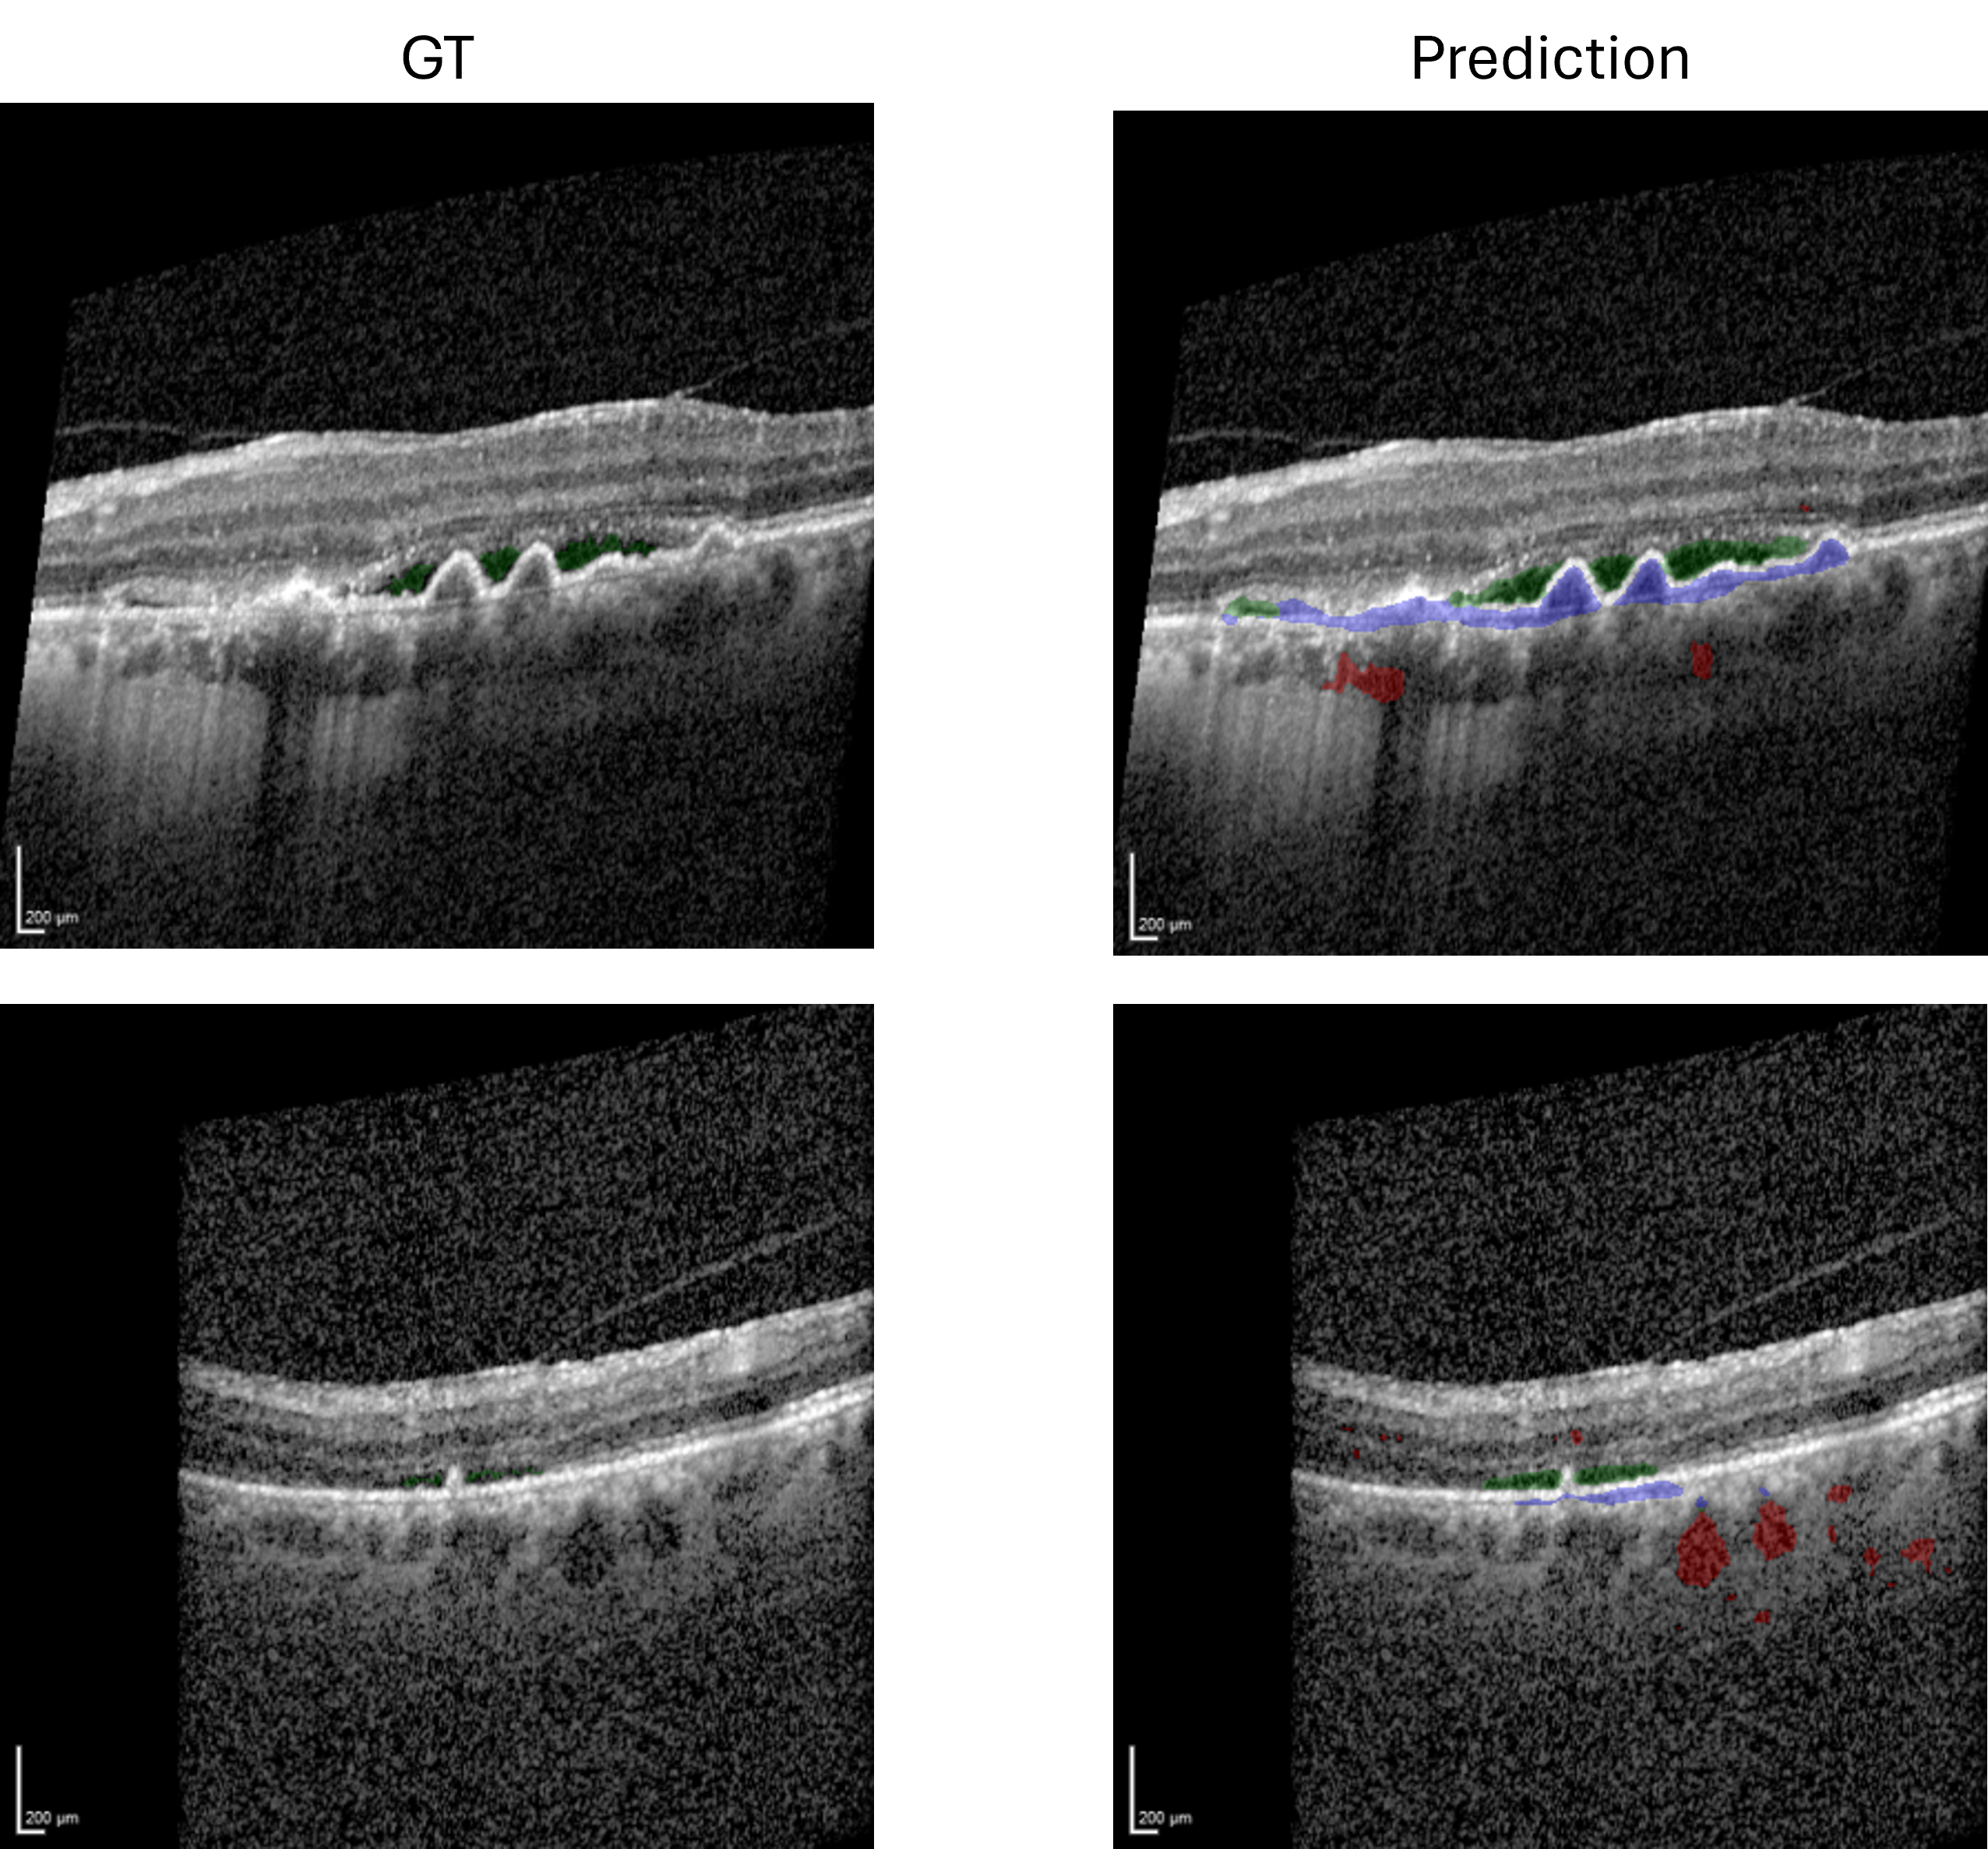
\includegraphics[width=0.75\linewidth]{figures/CHUSJSegmentationOnNoisyScans.png}
	\caption{Fluid segmentations performed by the multi-class model in noisy B-scans from the CHUSJ dataset.}
	\label{fig:CHUSJSegmentationOnNoisyScans}
\end{figure}

\section{Intermediate Slice Synthesis}\label{IntermediateSliceSynthesis}

This section presents the results obtained in the generation of intermediate B-scans between two consecutive real slices. In this section, the images generated using two different generative models are compared: the GAN and the U-Net.
\par
The comparison between these different methods is mainly qualitative, as the quality and perception of the images are prioritized over the calculated metrics, since the realism of the images and the performance of segmentation models on the generated slices are significantly affected by the appearance of the images.
\par
Nevertheless, the GANs trained on different folds are still compared through PSNR and SSIM, as a way to objectively select the best performing model for the \ref{FluidVolumeEstimation} Fluid Volume Estimation experiments.
\par
The comparison between these metrics and other articles in the literature is not possible. The only article of intermediate slice synthesis applied in OCT, developed by \textcite{Lopez2023}, does not evaluate the generated slices using these metrics. The articles in other imaging techniques such as CT and MRI have significantly different levels of noise and the values attained in these metrics in OCT are, therefore, very different.

\subsection{Experiment 3 - Intermediate Slices Synthesis Using a GAN}

In Experiment 3, a GAN was trained with the objective of generating the intermediate slice between a pair of two known and consecutive slices. In Table \ref{tab:Experiment1Metrics}, the PSNR and SSIM are shown for each fold in which the network was trained.

\begin{table*}[!ht]
	\caption{PSNR and SSIM in every device, for the generated slices in every validation fold.}
	\centering
	\resizebox{\textwidth}{!}{\begin{tabular}{|c|c|cccc|c|cccc|c|}
		\hline
		\multirow{2}{*}{\textbf{Run}} & \multirow{2}{*}{\textbf{VF}} & \multicolumn{4}{c|}{\textbf{PSNR}} & \multirow{2}{*}{\textbf{PSNR}} & \multicolumn{4}{c|}{\textbf{SSIM}} & \multirow{2}{*}{\textbf{SSIM}} \\ \cline{3-6} \cline{8-11}
		&  & \textbf{Cirrus} & \textbf{Spectralis} & \textbf{T-1000} & \textbf{T-2000} &  & \textbf{Cirrus} & \textbf{Spectralis} & \textbf{T-1000} & \textbf{T-2000} &  \\ \hline
		\textbf{Run 1} & 2 & \multicolumn{1}{c|}{\textbf{20.64}} & \multicolumn{1}{c|}{24.42} & \multicolumn{1}{c|}{21.56} & \multicolumn{1}{c|}{22.51} & \textbf{21.92} & \multicolumn{1}{c|}{\textbf{0.193}} & \multicolumn{1}{c|}{0.482} & \multicolumn{1}{c|}{0.177} & \multicolumn{1}{c|}{0.250} & \textbf{0.260} \\
		\textbf{Run 2} & 3 & \multicolumn{1}{c|}{20.44} & \multicolumn{1}{c|}{24.58} & \multicolumn{1}{c|}{21.63} & \multicolumn{1}{c|}{22.24} & 21.69 & \multicolumn{1}{c|}{0.181} & \multicolumn{1}{c|}{0.484} & \multicolumn{1}{c|}{0.188} & \multicolumn{1}{c|}{0.246} & 0.247 \\
		\textbf{Run 3} & 4 & \multicolumn{1}{c|}{20.40} & \multicolumn{1}{c|}{\textbf{24.93}} & \multicolumn{1}{c|}{\textbf{21.95}} & \multicolumn{1}{c|}{\textbf{22.56}} & 21.91 & \multicolumn{1}{c|}{0.175} & \multicolumn{1}{c|}{\textbf{0.498}} & \multicolumn{1}{c|}{\textbf{0.228}} & \multicolumn{1}{c|}{\textbf{0.263}} & \textbf{0.257} \\
		\textbf{Run 4} & 0 & \multicolumn{1}{c|}{} & \multicolumn{1}{c|}{} & \multicolumn{1}{c|}{} & \multicolumn{1}{c|}{} &  & \multicolumn{1}{c|}{} & \multicolumn{1}{c|}{} & \multicolumn{1}{c|}{} &  &  \\
		\hline
		\hline
		\textbf{Set 1} & - & \multicolumn{1}{c|}{} & \multicolumn{1}{c|}{} & \multicolumn{1}{c|}{} & \multicolumn{1}{c|}{} &  & \multicolumn{1}{c|}{} & \multicolumn{1}{c|}{} & \multicolumn{1}{c|}{} & \multicolumn{1}{c|}{} &  \\ \hline
	\end{tabular}}
	\label{tab:Experiment1Metrics}
\end{table*}

One of the trends that becomes evident when looking at this table is the difference in results between devices, which is constant across independent of the fold in which it was trained.
\par
In every fold, the scans generated with the Spectralis device show better values both in PSNR and SSIM, while those obtained with Cirrus are significantly worse. This is tied to the characteristics of the images obtained with each device. In Spectralis, the inter-slice distance is larger than in Cirrus, but this is compensated by the better B-scan quality, contrast, and reduced levels of noise. The opposite happens in Cirrus, as the B-scans are noisier and with a decent contrast, but separated by a smaller distance. In Topcon, the distance is similar to the Cirrus, but presents less noise with worse contrast. 
\par
As the speckle noise is hard to predict due to its random nature, the performance metrics are worse in the scans with more noise. These metrics compare the similarity between different images at a pixel level and in noisy regions, which occupy most of the B-scan, the differences at a pixel-level between generated and real images are significant, even if the differences are almost imperceptible.
\par
In other imaging techniques like MRI and CT, the noise levels are much less significant than OCT, resulting in better PSNR and SSIM values, that directly translate to image quality.
\par
When comparing the results across different runs, it turns out that the performance changes very slightly when the training data differs. Unlike the segmentation task, where the results in different validation folds were harshly affected by the fluid content present in the OCT volumes that compose them, the generation task appears indifferent to the random distribution of fluid.
\par
In the segmentation task, the model and evaluation focused solely on the fluid, which is a small portion of the image, while in generation the model attempts to accurately generate the whole scan as similar to the target slice as possible. By considering the entirety of the B-scan, less of the performance is affected by the fluid region, which is why the distribution of fluid does not affect the overall performance as much as it did in segmentation, even if it is the most difficult section to generate.
\par
Despite the significant worse performance in Cirrus when compared to Spectralis, the visual similarity between generated images and real images, at an human level, is not very different. In Figure \ref{fig:GeneratedSlicesCirrusVsSpectralis}, two pairs of real and generated images from these devices are shown.
\par
The generated slices capture the rough idea of the image, especially the retinal layers, but miss on the small details such as noise patterns, and brighter and unexpected structures. Overall, the generated Cirrus scan captures the details present in the real image better than the Spectralis. For example, the structures which appear in the choroid are similar to the original slice in the generated Cirrus slice, while in Spectralis these structures appear blurred. However, due to the highest levels of noise, this does not translate to better PSNR or SSIM.

\begin{figure}[!ht]
	\centering	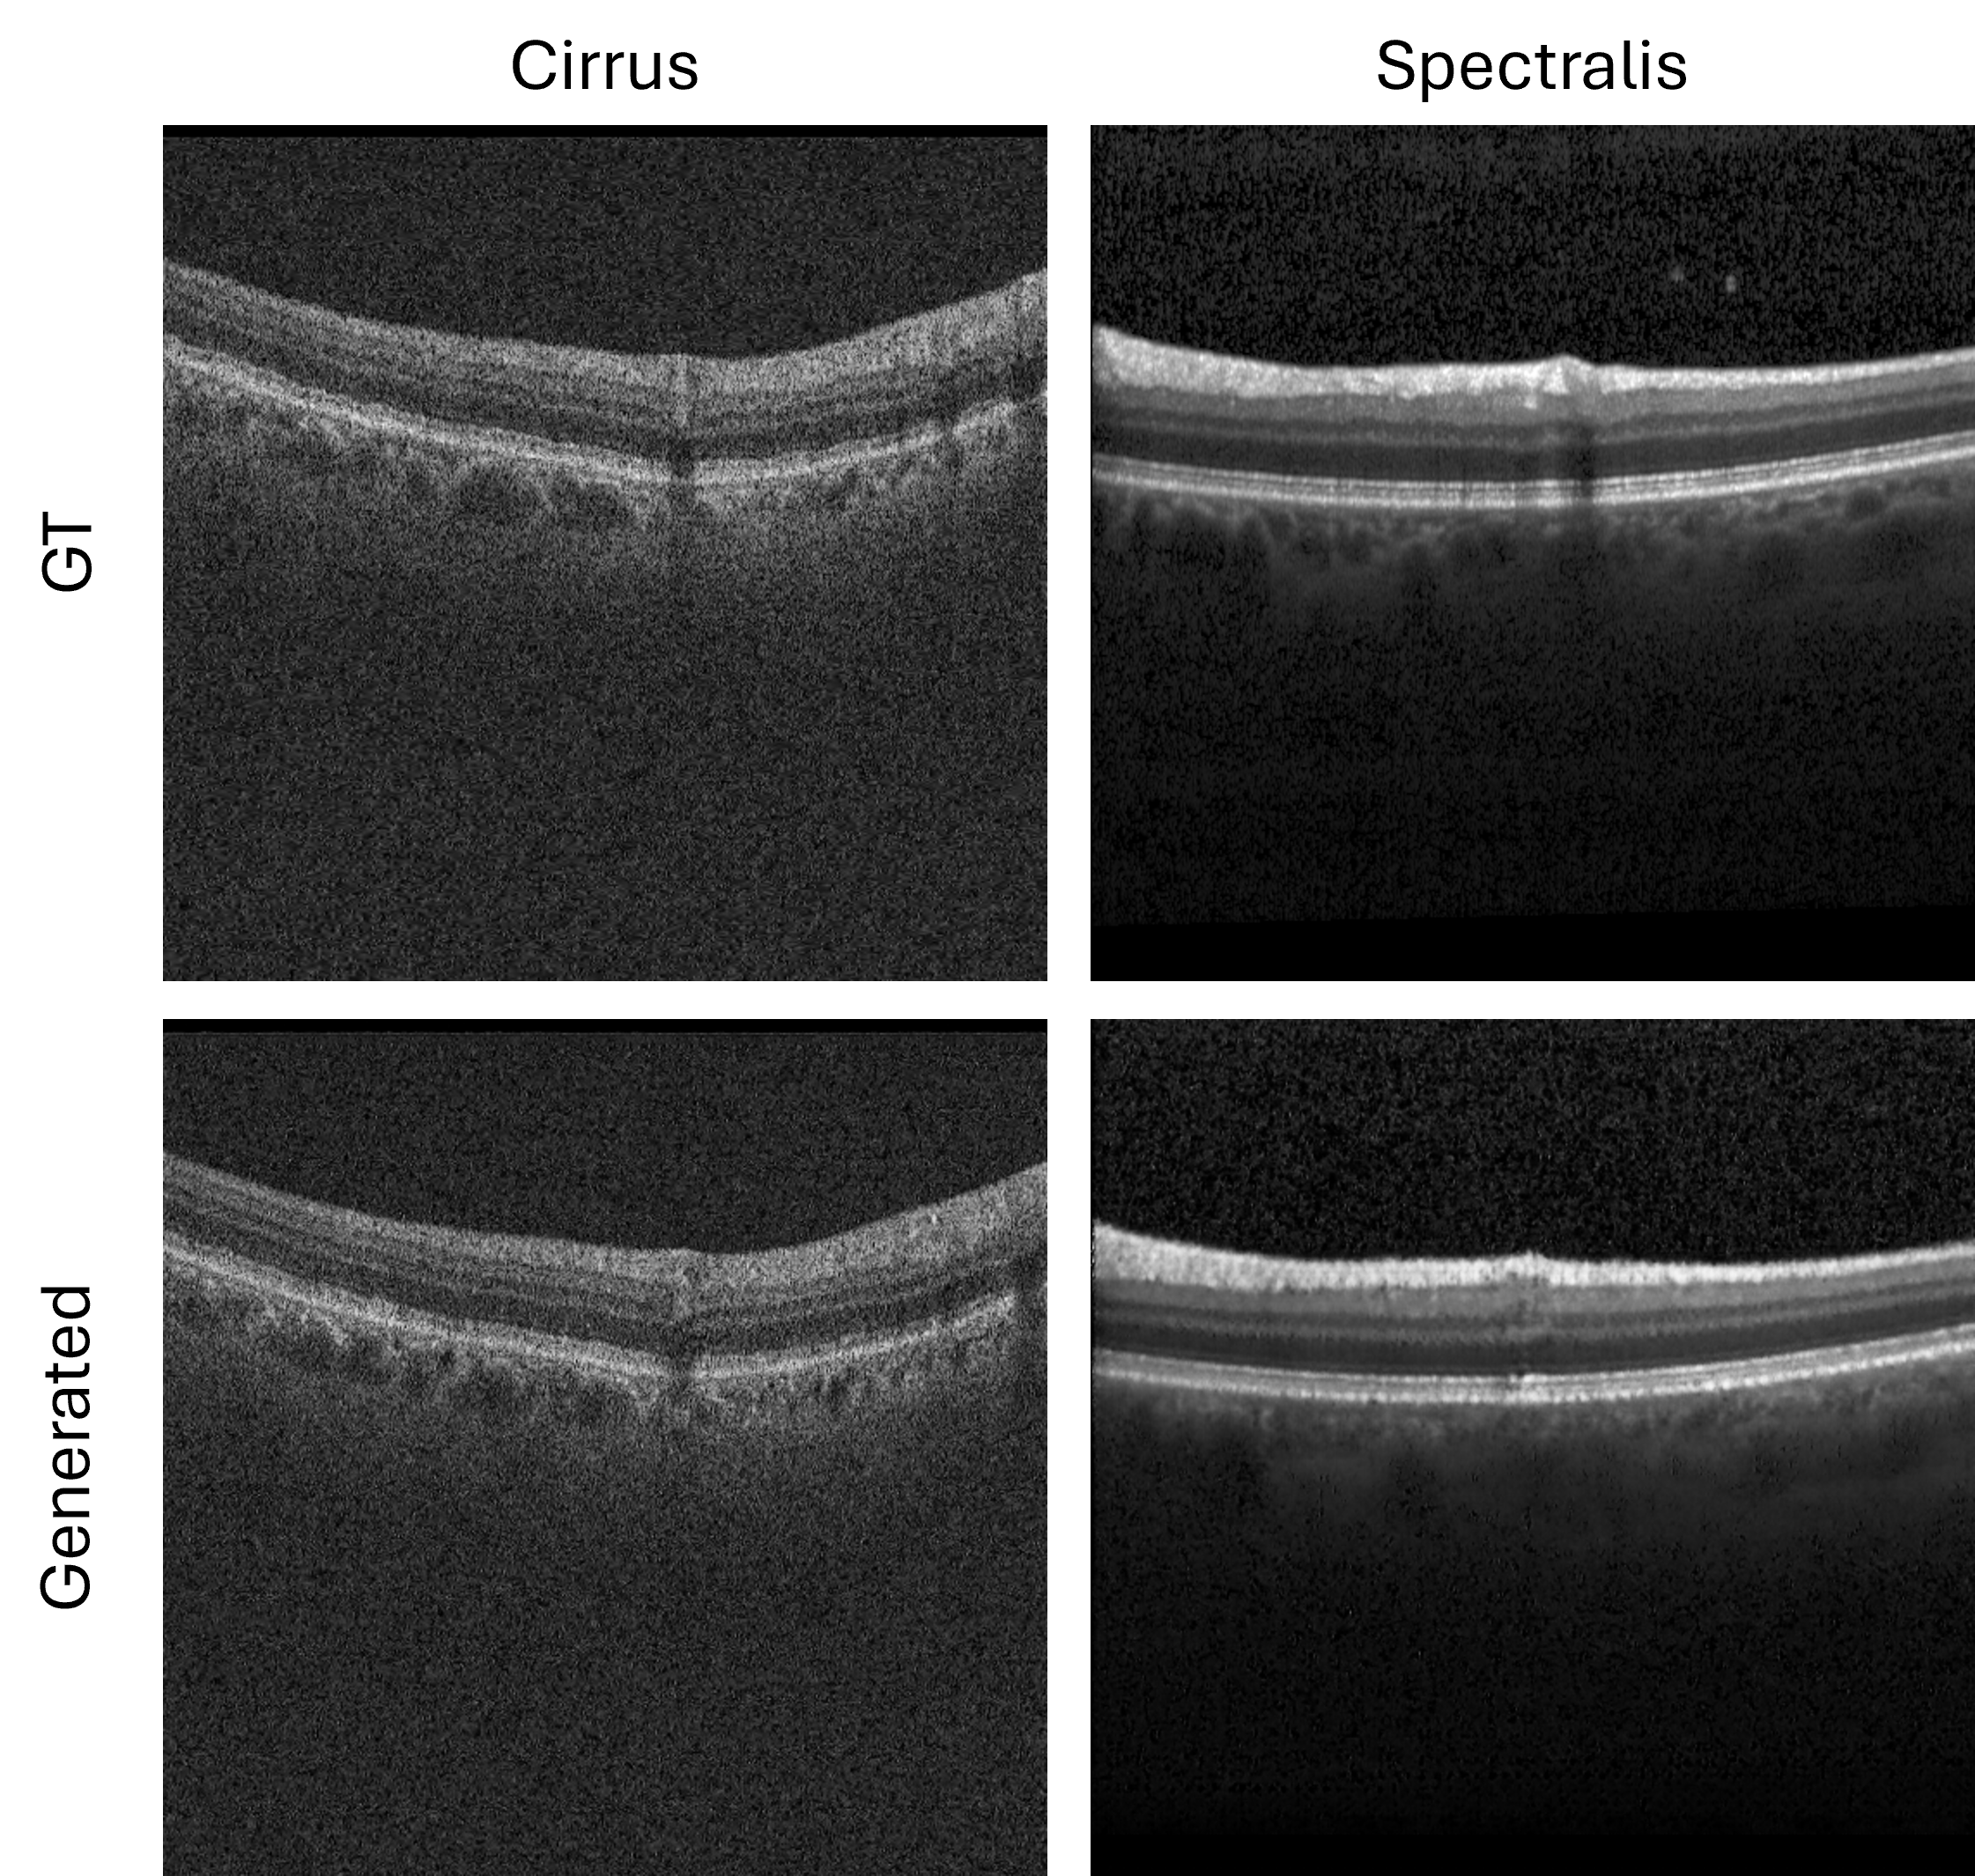
\includegraphics[width=0.75\linewidth]{figures/GeneratedSlicesCirrusVsSpectralis.png}
	\caption{Example of two pairs of generated slices, one from Cirrus and one from Spectralis, which capture the retinal layers.}
	\label{fig:GeneratedSlicesCirrusVsSpectralis}
\end{figure}

The differences in performance exhibited in this image regarding the representation of details are related with the inter-slice distance of the OCT volumes. In Cirrus, where the inter-slice distance is smaller than in Spectralis, the differences between the surrounding slices and the middle slice are smaller. Therefore, it is easier for the model to predict the content in the middle slice of a Cirrus volume than it is in Spectralis. Figure \ref{fig:TransitionBetweenConsecutiveBScansCirrusVsSpectralis} shows the surrounding slices of the B-scans generated in Figure \ref{fig:GeneratedSlicesCirrusVsSpectralis}. It becomes evident the difference in the transitions between the surrounding slices and the intermediate slices. For example, in the choroid region, where the generative model output was blurred, the structures that appear in the previous slice are significantly different in the following slice. In the same region, the Cirrus B-scans present a much smoother transition, which results in an improved and more realistic output.

\begin{figure}[!ht]
	\centering	\includegraphics[width=1.0\linewidth]{figures/TransitionBetweenConsecutiveBScansCirrusVsSpectralis.png}
	\caption{Surrounding slices of the B-scans generated in Figure \ref{fig:GeneratedSlicesCirrusVsSpectralis}.}
	\label{fig:TransitionBetweenConsecutiveBScansCirrusVsSpectralis}
\end{figure}

However, it is of our best interest to generate slices that accurately represent the fluid regions, on top of being visually similar to the original scans, as an accurate representation of the generated fluids, directly translates to a better performance in the segmentation of fluid in theses slices. 
\par
An accurate segmentation of fluid in generated B-scans is mainly dependent on the overall quality of the image and its resemblance to the images in which it was trained and the aspect of the generated fluid regions.
\par
Similar to what was seen in other structures such as the choroid and the retinal layers, the quality of the generated fluid regions is dependent on the distance between scans more than the contrast and levels of noise in the image. However, the characteristics of each fluid also influence its generation, mainly because of their progression between consecutive slices. For example, the SRF usually appears in a more homogeneous and continuous shape, making it easier to predict its characteristics given the information of the surrounding slices. Contrasting, the IRF usually appears in small and irregular shapes, commonly separated by small retinal tissue. In consecutive slices, the small IRF regions quickly change its shape and may even merge together, which makes it harder to predict. The PED fluid can appear both as small inconsistent fluid like the IRF, but most commonly as a large and predictable region, similar to SRF.
\par
An example of each generated fluid is seen in Figure \ref{fig:GeneratedSlicesWithFluid}, where the generation of IRF confuses the model while the fake SRF and PED appear similar to its GT. The characteristics of these generated fluids is particularly important to understand the consequences that slice generation has in fluid volume estimation.

\begin{figure}[!ht]
	\centering	\includegraphics[width=1.0\linewidth]{figures/GeneratedSlicesWithFluid.png}
	\caption{Examples of generated B-scans with fluid.}
	\label{fig:GeneratedSlicesWithFluid}
\end{figure}

In this figure, it becomes evident that the generation of SRF and PED, seen in Topcon example, is a much simpler task than the generation of any other fluid. In fact, the overall structure of this region has been very accurately preserved, apart from small visual details.
\par
The generation of IRF, however, appears more troublesome, particularly in Spectralis. In this last device, while in the GT the fluid regions appear individually separated by small retinal tissue, in the generated images the structures surrounding the fluid appear deformed, making it hard to understand which region is fluid and which is retina. It is interesting to note that the SRF shape stays consistent, highlighting that this fluid changes much slower as the slices progress than IRF. In Cirrus, the model preserves the IRF structures accurately, apart from the small and thin sections of retinal tissue which separate the fluid regions, where some merging occurs. This small details occur due to the target slice being located between one slice that contains this small tissues and another that does not. Nevertheless, the characteristics of this fluid are much more similar to the GT than in Spectralis, emphasizing the impact that the inter-slice distance has in slice generation.
\par
The poor generation of IRF is also partially related with the loss used to train the GAN. Since this network was adapted from a video frame interpolation application, the method is not prepared for datasets that contain as much noise as OCT does. In the video use case, it makes sense to use a loss function that primarily evaluates the images at a pixel level, while being complimented by a perception component, which is the adversarial loss, that corresponds to the capability of a fake image fooling the discriminator. However, in OCT, the speckle that corrupts the image makes it considerably more difficult to optimize a network to generate images that are similar at a pixel level, since this noise is impossible to predict. Therefore, as the network attempts to reproduce the noise that occupies most of the B-scans, it does not apply as much attention to the fluid as it should, particularly in IRF that needs it more. Ultimately, this results in visually similar images in the matters of noise and retinal layers, but worse in the generation of fluids.
\par
To perform the generation of intermediate slices in Experiment 6, the model from Run 3 was selected, as it obtained the best metrics in PSNR and SSIM.

\subsection{Experiment 4 - Intermediate Slices Synthesis Using a U-Net}

The second experiment in the scope of generating intermediate slices was performed using a U-Net and only a single model was trained. Examples of B-scans generated using this model are shown in Figure \ref{fig:GenerativeUNetResults}.

\begin{figure}[!ht]
	\centering	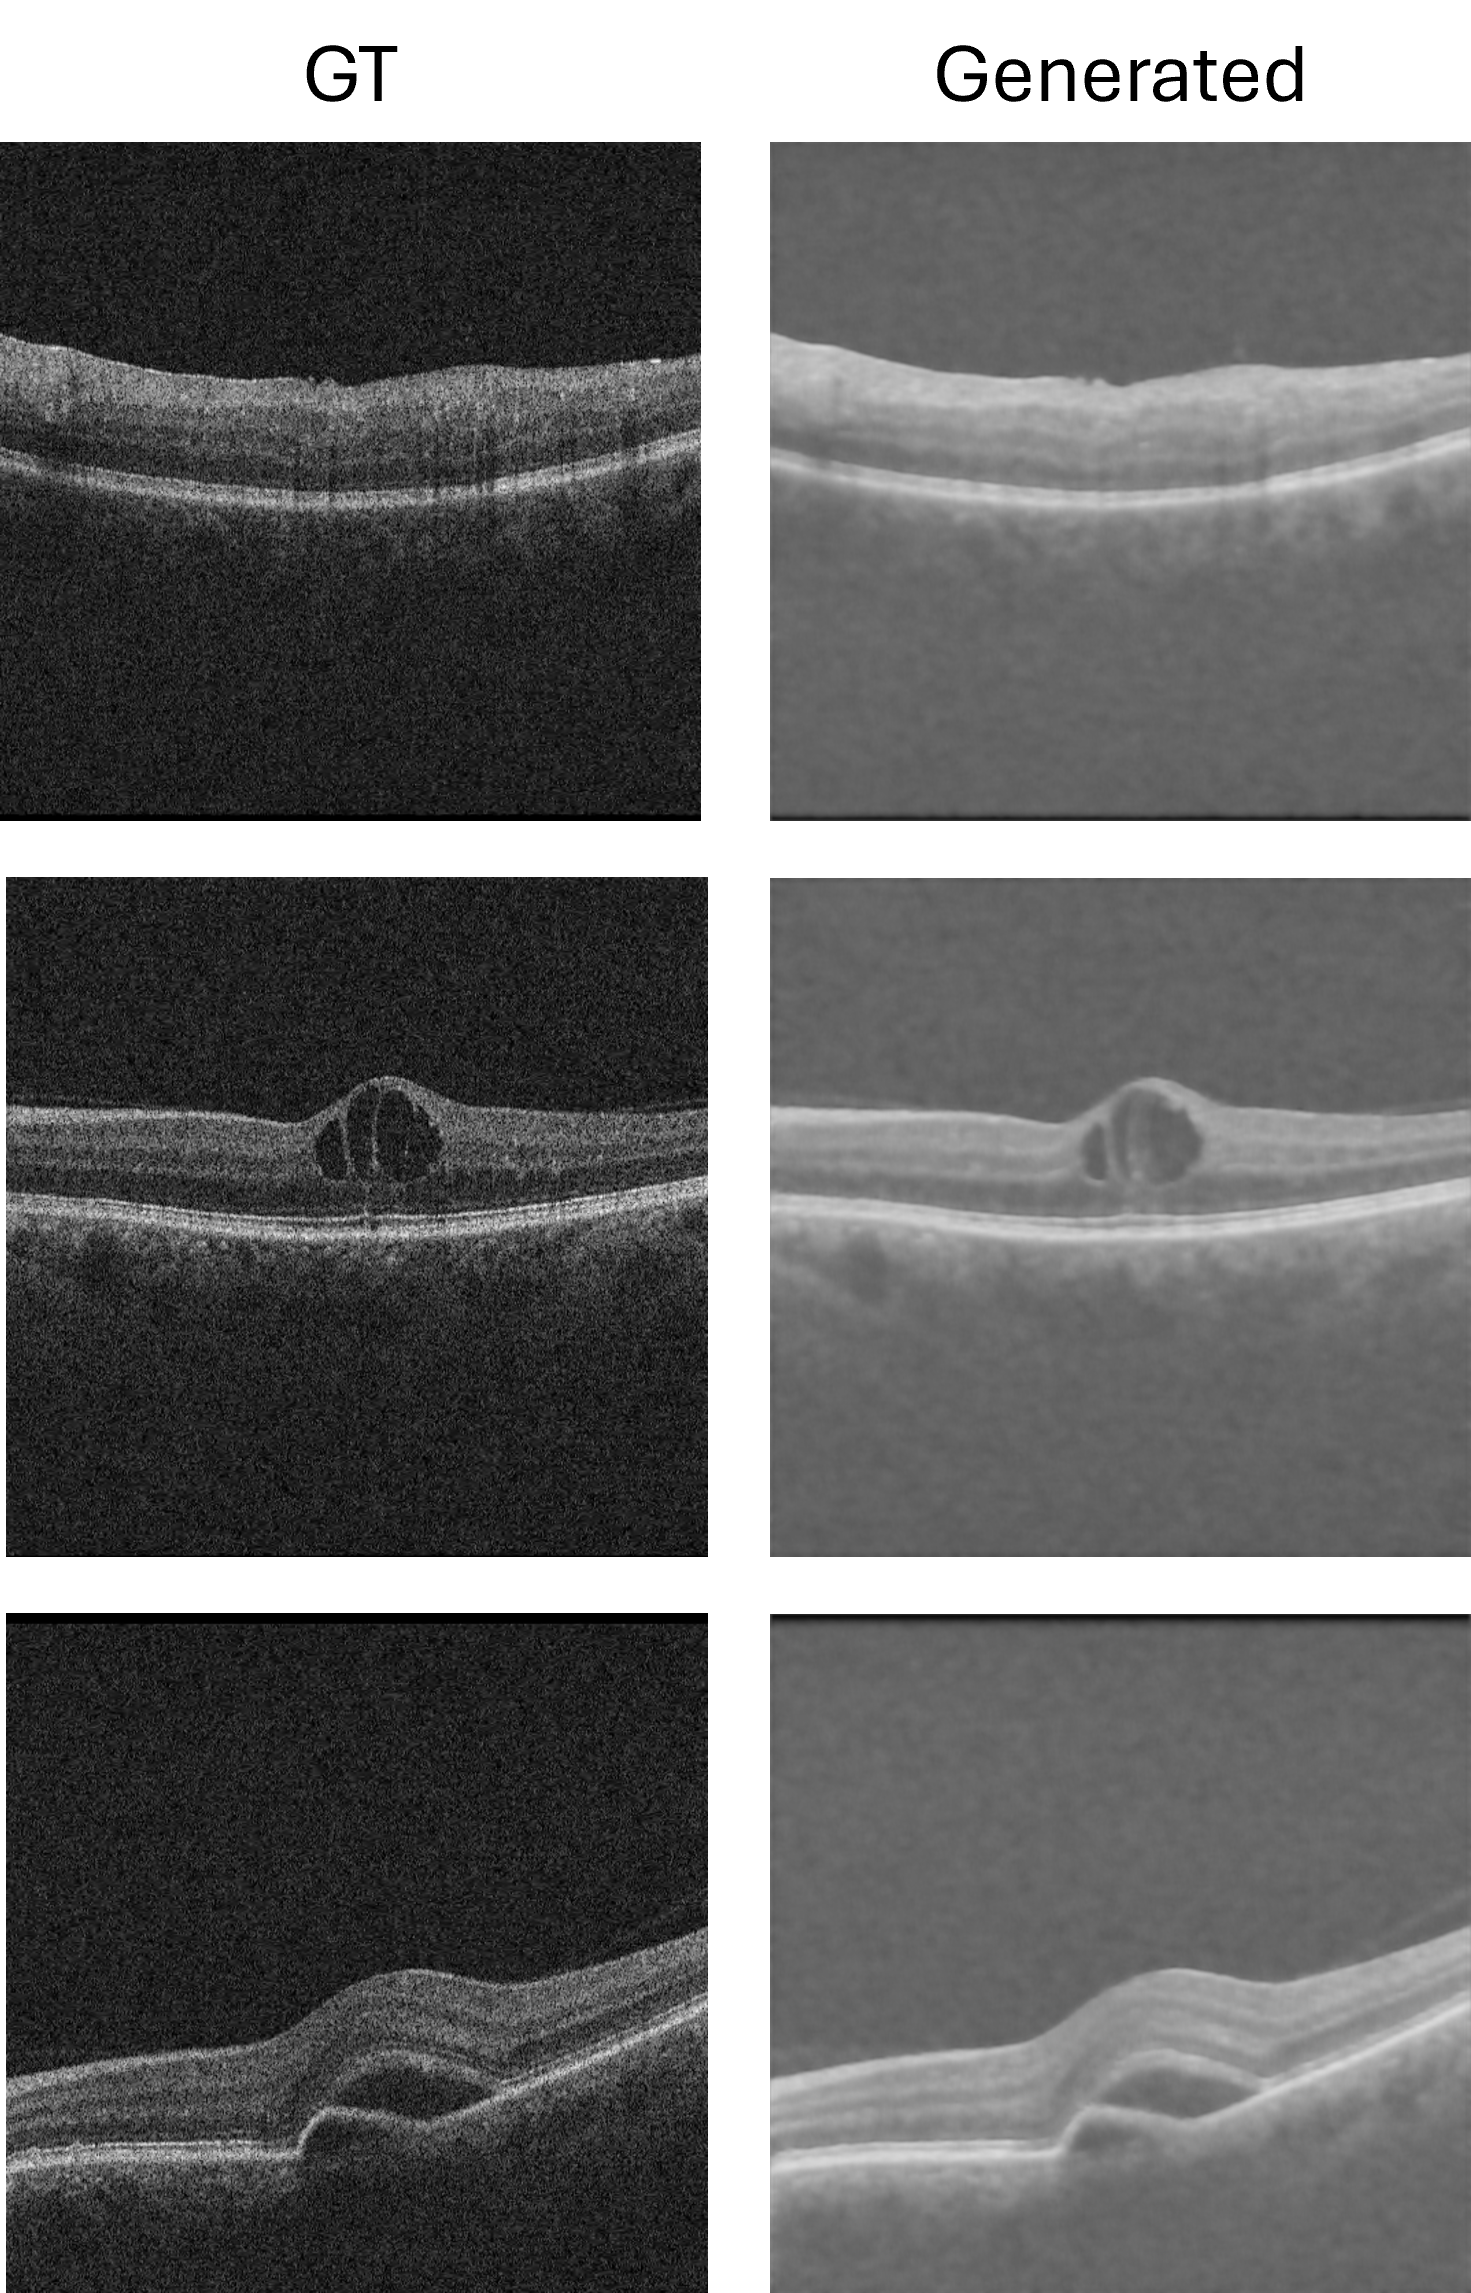
\includegraphics[width=1.0\linewidth]{figures/GenerativeUNetResults.png}
	\caption{B-scans generated using the U-Net. The images on the left show the original B-scan while those on the left are the corresponding generated slices.}
	\label{fig:GenerativeUNetResults}
\end{figure}

When evaluating the quality of the generated images, a noticeable lack of realism is observed, as these images often resemble a smoothed approximation of the GT. Despite the similarity in architecture between the generator used in the GAN and the U-Net, the second model could not reach a performance comparative with the GAN. The U-Net faces three significant challenges: its loss is not representative, it is trained with large images, and does not have a discriminator.
\par
The main problem comes from the network not being able to produce realistic images by reducing the loss. While the MAE is a good metric to compare two images, it does not perform well as the loss of a generative model in OCT. The reason MAE is insufficient to motivate the model to properly generate images is because the easiest, fastest, and safest way the model has of reducing the MAE in training is by creating blurred images, especially in noisy regions of the image.
\par
While these blurred images are not as realistic as the GT, the MAE is not as bad as it would be in case the model attempted to create images that are more visually similar to the real images. When dealing with OCT, a large portion of the image contains speckle noise, which is difficult to predict. Therefore, reaching results that are visually similar includes the representation of speckle noise in the intermediate slices, which results in a worse MAE.
\par
It is due to the inability of regularizing a generative model alone that the MAE was combined with other losses in the previous experiment. While this loss is important to represent the direct similarity between two images, it fails to capture the perception of the structures and visual similarity between images. This is why the MAE loss was attributed such small weight in Experiment 3.
\par
When comparing to the work by \textcite{Nishimoto2024}, in which this experiment was inspired, the dataset presented almost no noise in most images. Therefore, the generative task was simpler and the model was able to generalize significantly better, as the MAE was enough to promote an accurate slice interpolation. However, when facing images with more noise, caused by the presence of metal artifacts in the CT, the generation of slices performed worse than the linear interpolation. Therefore, while this model generates good images when the slices have almost no noise present, it lacks the robustness to generate images where noise appears.
\par
The use of a U-Net to generate intermediate B-scans is also harmed by the input it received. While in the GAN, the discriminator and the generator were trained with small patches of 64 $\times$ 64, the U-Net was trained with the entire image. Consequently, this motivates the U-Net to focus on the more general details of the image, rather than on the finer characteristics, as done in the GAN, ultimately contributing to the generation of less realistic images.
\par
Lastly, this model lacks the regularization brought by an external network which is, in the case of a GAN, the discriminator. With the inclusion of a discriminator, a perceptual component is added to the loss. This motivates the model to produce the images that are not only similar to the pixel level, but also visually accurate. Therefore, this results in an image where the textures are more realistic, even if the difference at a pixel level is worse.
\par
Nevertheless, it is seen in Figure \ref{fig:GenerativeUNetResults} that the borders of the fluid regions are preserved. This representation is not as difficult as the other components of the B-scan, but is better in the generation of SRF and PED, where the fluid regions are more homogeneous. In IRF, the shape of the fluid is bounded by the deformations caused inside the retina, which makes it harder to generate, leading to the fluid regions appearing significantly different from what is expected. Furthermore, the goal of generating intermediate slices was not only to generate images that are similar in the fluid regions, but also in the overall image, and for this reason, no other generative U-Net model was trained. The accurate delimitation of the generated fluids does not directly translate to a good segmentation performance in the created slices, since the image's overall different appearance could impact the segmentation model's performance.

\section{Fluid Volume Estimation}\label{FluidVolumeEstimation}

The experiments discussed in this section relate to the estimation of fluid volume using the segmentation masks of each B-scan in an OCT volume. In both experiments, the fluid volumes predicted using the segmentation models are compared to the fluid volumes calculated using the GT masks from the dataset, in the reserved fold. 
\par
This fold had not been seen by any segmentation or generative model and the GT fluid masks are available for all OCT scans.
\par
The discussion of these experiments aim to understand the applicability of enhancing the resolution of an OCT volume and how that affects the total fluid volume estimated, among other aspects such as the perception of the generated slices by the segmentation model.
\par
The results are shown in tables where for each considered OCT volume, the fluid volume estimated for each fluid type (IRF, SRF, and PED) is presented in mm$^{3}$. At the end of each table, the MAE is shown to resume the differences between the GT fluid volumes and the prediction.
\par
In Experiment 6, the Dice coefficient for the predict segmentation masks in fully generated OCT volumes is shown, allowing the comparison between the segmentation model's performance in real data and generated data, providing an insight on which fluids are affected the most the generation.
\par
Lastly, scatter plots are shown for each comparison between predictions, where the each of the fluids' volumes calculated for each OCT scan are compared with each other, providing an intuitive and visual representation of the differences associated with the used data.

\subsection{Experiment 5 - Fluid Volume Estimation Using Predicted Masks in Real OCT Volumes}
In Experiment 5, the fluid volume was calculated for each type of fluid in the OCT volumes from the reserved fold, using the previously described in \ref{Methods} Materials and Methods. The volume of each fluid, for each OCT volume in the reserved fold, is shown in Table \ref{tab:FluidVolumesExperiment5}, in mm$^{3}$. In Figure \ref{fig:FluidVolumeScatterExperiment5}, the comparison between the values calculated using the GT masks and the masks predicted by the segmentation model is shown, using the values present in this table.

\begin{table*}[!ht]
	\centering
	\caption{Volume of each fluid calculated for the masks segmented in the RETOUCH (GT) and the masks segmented by the best segmentation model from Experiment 1 and 2 (P). The volumes correspond to the total fluid volume in the OCT scan, in mm$^{3}$.}
	\begin{tabular}{|c|c|cc|cc|cc|}
		\hline
		\multirow{2}{*}{\textbf{Vendor}} & \multirow{2}{*}{\textbf{Volume}} & \multicolumn{2}{c|}{\textbf{IRF}} & \multicolumn{2}{c|}{\textbf{SRF}} & \multicolumn{2}{c|}{\textbf{PED}} \\ \cline{3-8} 
		& & \textbf{GT} & \textbf{P} & \textbf{GT} & \textbf{P} & \textbf{GT} & \textbf{P} \\ \hline
		 Cirrus & TRAIN002 & 0.228 & 0.373 & 0.008 & 0.013 & 0.000 & 0.000 \\
		 Cirrus & TRAIN012 & 0.000 & 0.001 & 0.704 & 0.673 & 0.888 & 0.946 \\
		 Cirrus & TRAIN014 & 0.000 & 0.000 & 0.517 & 0.575 & 0.332 & 0.252 \\
		 Cirrus & TRAIN016 & 0.771 & 1.129 & 0.000 & 0.000 & 0.000 & 0.000 \\
		 Spectralis & TRAIN027 & 0.937 & 1.071 & 0.096 & 0.132 & 0.000 & 0.001 \\
		 Spectralis & TRAIN033 & 0.254 & 0.380 & 0.314 & 0.307 & 0.367 & 0.471 \\
		 Spectralis & TRAIN039 & 0.622 & 0.839 & 0.000 & 0.000 & 0.000 & 0.000 \\
		 Spectralis & TRAIN042 & 0.002 & 0.009 & 1.900 & 1.875 & 0.603 & 0.771 \\
		 Spectralis & TRAIN048 & 0.328 & 0.446 & 0.000 & 0.008 & 0.000 & 0.000 \\
		 T-2000 & TRAIN062 & 0.047 & 0.058 & 0.000 & 0.000 & 0.000 & 0.000 \\
		 T-1000 & TRAIN063 & 0.000 & 0.011 & 0.747 & 0.568 & 0.034 & 0.110 \\
		 T-1000 & TRAIN064 & 0.058 & 0.060 & 0.000 & 0.003 & 0.000 & 0.075 \\
		 T-2000 & TRAIN067 & 0.188 & 0.170 & 0.000 & 0.000 & 0.000 & 0.000 \\
		 T-2000 & TRAIN068 & 0.406 & 0.550 & 0.004 & 0.006 & 0.000 & 0.008 \\ \hline
		 \multicolumn{2}{|c|}{\textbf{MAE}} & \multicolumn{2}{c|}{0.092} & \multicolumn{2}{c|}{0.025} & \multicolumn{2}{c|}{0.041} \\ \hline
		 
	\end{tabular}
	\label{tab:FluidVolumesExperiment5}
\end{table*}

\begin{figure}[!ht]
	\centering	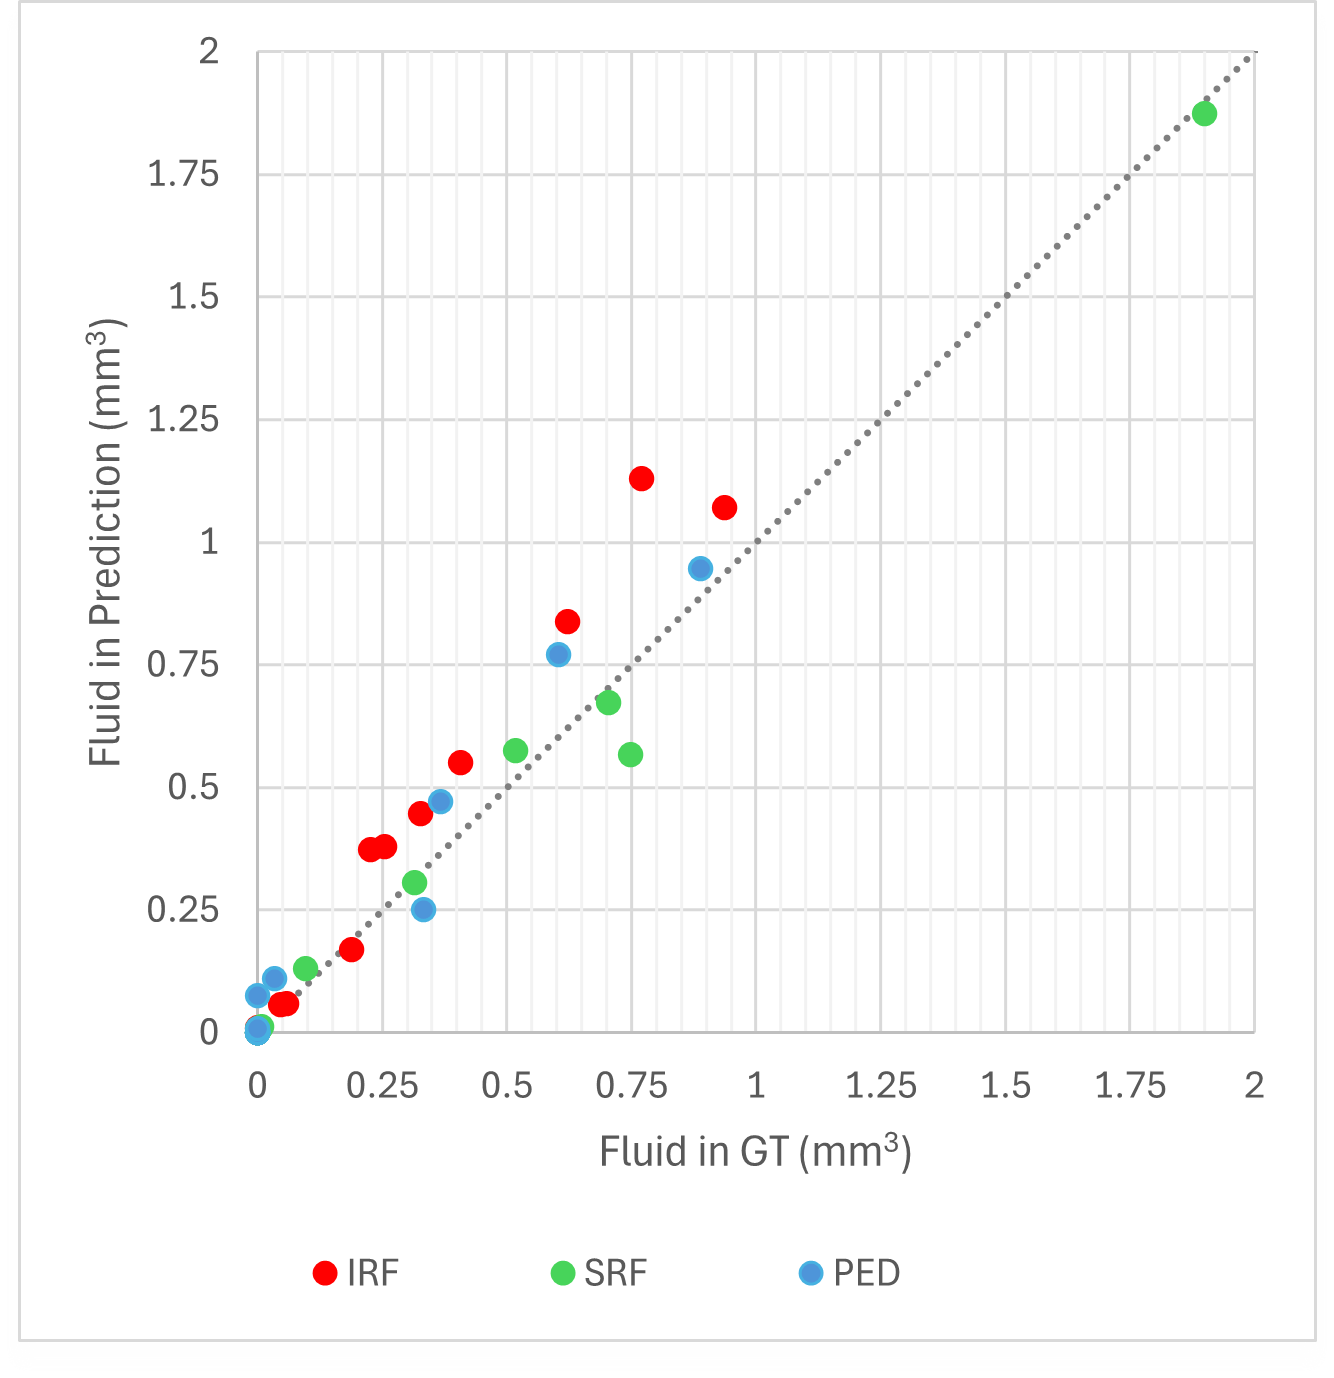
\includegraphics[width=0.66\linewidth]{figures/FluidVolumeScatterExperiment5.png}
	\caption{Volume estimated for each fluid in OCT volume using the masks predicted by the segmentation model compared with the volumes calculated using the GT masks. The OCT scans considered are the same as in \ref{tab:FluidVolumesExperiment5} and the gray line marks the points in which the fluid volume in the GT is equal to the predicted.}
	\label{fig:FluidVolumeScatterExperiment5}
\end{figure}

The values shown in this table reveal the similarity between the fluid volumes estimated with the RETOUCH GT masks and the masks predicted by the selected segmentation model. However, there are some outliers and evident trends seen.
\par
For example, in IRF, there are multiple examples where the predicted quantity of fluid is significantly larger than the real quantity, such as in TRAIN002, TRAIN016, TRAIN039, and TRAIN048. These outliers appear mostly on Cirrus and Spectralis. In these vendors, the IRF presents more diverse shapes and deformity of the retina, which makes segmentation significantly harder than in Topcon, where the IRF appears much smaller and without deformation.
\par
In SRF and PED, the differences between the true and predicted quantity are not so significant, with the largest discrepancies being the SRF and PED in TRAIN063. The shape of these fluids in the OCT volumes present in this fold are more consistent with those seen in training, hence resulting in a more accurate segmentation.
\par
Overall, the volumes predicted in scans with considerable quantities of fluid tend to differ more with its GT. This happens due to the deformation in the retina that is associated with large quantities of fluid, making it harder to predict the segmentation masks.
\par
Nonetheless, the fluid prediction in slices with little to no fluid tends to be accurate, highlighting the good specificity and segmentation of small fluids previously seen in the segmentation model.
\par
Regarding the performances per vendor, there is no significant differences to note, as most of the differences in noticeable in these results are related to the different characteristics of the patients in each OCT.
\par
It is interesting to note that in discrepancies between the real volume and the predicted volume, the segmentation model tends to overpredict fluid, which is associated with the oversegmentation trend seen in the predictions performed by this model. This is an important aspect to note, as it is rooted to the segmentation criteria used in the training data, the RETOUCH dataset. This trend further justifies the oversegmentations seen by the model in the CHUSJ dataset.
\par
In the following subsection, the results shown in Table \ref{tab:FluidVolumesExperiment5} will be compared with the estimated fluid volumes obtained using only generated slices and in an enhanced volume, where between every known slice another slice is generated.

\subsection{Experiment 6 - Fluid Volume Estimation Using Predicted Masks in Generated and Super-resolved OCT Volumes}

The results obtained regarding fluid estimation with generated slices, in the scope of Experiment 6, are shown in Table  \ref{tab:FluidVolumesExperiment6}. In this table, four different fluid volume estimates are shown for each OCT volume in the reserved fold, separately for each fluid type. The first estimate, ``GT'', is obtained using the unchanged B-scans from each volume and the fluid masks provided in the RETOUCH dataset. The second estimate, ``P'', corresponds to the fluid masks predicted by the segmentation model in the unchanged B-scans of the same OCT volumes. Both predictions and fluid estimations were already presented in Experiment 5. In the third estimate, ``G'', the B-scans from the RETOUCH dataset are substituted with their corresponding generated B-scan, obtained using the selected GAN model. In these generated scans, the segmentation model predicts the fluid masks, from which the estimated volumes presented in this table are obtained. Lastly, in the fourth estimation ``E'', the original OCT volumes from the RETOUCH dataset are enhanced, as a B-scan is generated between every two consecutive slices. The segmentation model predicts the fluid masks both in the original and generated slices.
\par
In the last three rows of the table, multiple MAE are calculated to compare the results obtained in the multiple columns. The first row, shows the MAE between the estimations in the column ``GT'' and the estimations from the other columns. In the second row, the estimations performed using the segmentation model in column ``P'' are compared to the estimations made in the columns ``G'' and ``E'', while the third row compares the results obtained in these last two columns.

\begin{table*}[!ht]
	\centering
	\caption{Volume of each fluid calculated for the masks segmented in the RETOUCH (GT) and for the masks predicted by the best segmentation model in the original RETOUCH images (P), in the generated slices (G), and when the original dataset is enhanced, combining alternating the real images with B-scans generated between them (E). The volumes correspond to the total fluid volume in the OCT scan, in mm$^{3}$.}
	\resizebox{\textwidth}{!}{\begin{tabular}{|c|c|cccc|cccc|cccc|}
		\hline
		\multirow{2}{*}{\textbf{Vendor}} & \multirow{2}{*}{\textbf{Volume}} & \multicolumn{4}{c|}{\textbf{IRF}} & \multicolumn{4}{c|}{\textbf{SRF}} & \multicolumn{4}{c|}{\textbf{PED}} \\ \cline{3-14} 
		& & \textbf{GT} & \textbf{P} & \textbf{G} & \textbf{E} & \textbf{GT} & \textbf{P} & \textbf{G} & \textbf{E} & \textbf{GT} & \textbf{P} & \textbf{G} & \textbf{E} \\ \hline
		
 		Cirrus & TRAIN002 & 0.228 & 0.373 & 0.356 & 0.372 & 0.008 & 0.013 & 0.014 & 0.013 & 0.000 & 0.000 & 0.000 & 0.000 \\
 		
		Cirrus & TRAIN012 & 0.000 & 0.001 & 0.001 & 0.001 & 0.704 & 0.673 & 0.664 & 0.670 & 0.888 & 0.946 & 0.939 & 0.943 \\
		
		Cirrus & TRAIN014 & 0.000 & 0.000 & 0.001 & 0.003 & 0.517 & 0.575 & 0.561 & 0.572 & 0.332 & 0.252 & 0.207 & 0.227 \\
		
		Cirrus & TRAIN016 & 0.771 & 1.129 & 0.957 & 1.050 & 0.000 & 0.000 & 0.001 & 0.000 & 0.000 & 0.000 & 0.000 & 0.000 \\
		
 		Spectralis & TRAIN027 & 0.937 & 1.071 & 1.066 & 1.063 & 0.096 & 0.132 & 0.136 & 0.136 & 0.000 & 0.001 & 0.002 & 0.002 \\
 		
		Spectralis & TRAIN033 & 0.254 & 0.380 & 0.414 & 0.385 & 0.314 & 0.307 & 0.298 & 0.320 & 0.367 & 0.471 & 0.397 & 0.427 \\
		
		Spectralis & TRAIN039 & 0.622 & 0.839 & 0.726 & 0.779 & 0.000 & 0.000 & 0.002 & 0.000 & 0.000 & 0.000 & 0.000 & 0.000 \\
		
		Spectralis & TRAIN042 & 0.002 & 0.009 & 0.017 & 0.011 & 1.900 & 1.875 & 1.828 & 1.852 & 0.603 & 0.771 & 0.822 & 0.781 \\

		Spectralis & TRAIN048 & 0.328 & 0.446 & 0.336 & 0.398 & 0.000 & 0.008 & 0.013 & 0.009 & 0.000 & 0.000 & 0.001 & 0.001 \\

		T-2000 & TRAIN062 & 0.047 & 0.058 & 0.043 & 0.051 & 0.000 & 0.000 & 0.000 & 0.000 & 0.000 & 0.000 & 0.000 & 0.000 \\

		T-1000 & TRAIN063 & 0.000 & 0.011 & 0.007 & 0.010 & 0.747 & 0.568 & 0.507 & 0.546 & 0.034 & 0.110 & 0.111 & 0.108 \\
		
		T-1000 & TRAIN064 & 0.058 & 0.060 & 0.061 & 0.063 & 0.000 & 0.003 & 0.025 & 0.008 & 0.000 & 0.075 & 0.215 & 0.114 \\

		T-2000 & TRAIN067 & 0.188 & 0.170 & 0.137 & 0.160 & 0.000 & 0.000 & 0.000 & 0.000 & 0.000 & 0.000 & 0.000 & 0.000 \\

		T-2000 & TRAIN068 & 0.406 & 0.550 & 0.543 & 0.548 & 0.004 & 0.006 & 0.006 & 0.006 & 0.000 & 0.008 & 0.010 & 0.008 \\
		
		\hline
		\multicolumn{2}{|c|}{\textbf{MAE compared to GT}} & - & 0.092 & 0.067 & 0.079 & - & 0.025 & 0.036 & 0.029 & - & 0.041 & 0.052 & 0.043 \\ 
		\multicolumn{2}{|c|}{\textbf{MAE compared to P}} & - & - & 0.037 & 0.016 & - & - & 0.012 & 0.005 & - & - & 0.023 & 0.009 \\
		\multicolumn{2}{|c|}{\textbf{MAE compared to G}} & - & - & - & 0.022 & - & - & - & 0.009 & - & - & - & 0.014 \\ 
		\hline
		
	\end{tabular}}
	\label{tab:FluidVolumesExperiment6}
\end{table*}

In Figures \ref{fig:Experiment6GTvsAll}, \ref{fig:Experiment6PredictedVsAll}, and \ref{fig:Experiment6GeneratedVsEnhanced}, the estimated volumes shown in Table \ref{tab:FluidVolumesExperiment6} are plotted and compared with each other, providing a visual insight in the relationships between the estimated fluids, making the analysis easier. Figure \ref{fig:Experiment6GTvsAll} compares the volumes estimated using the GT masks with the volumes estimated in the other columns, ``P'', ``G'', and ``E''. Similarly, Figure \ref{fig:Experiment6PredictedVsAll} confronts the fluid volume estimations made using the fluid masks predicted by the segmentation model to the estimations made in columns ``G'' and ``E''. Finally, Figure \ref{fig:Experiment6GeneratedVsEnhanced} confronts the fluid volumes predicted in the generated dataset to the fluid volumes predicted in the enhanced dataset.

\begin{figure}[!ht]
	\centering	
	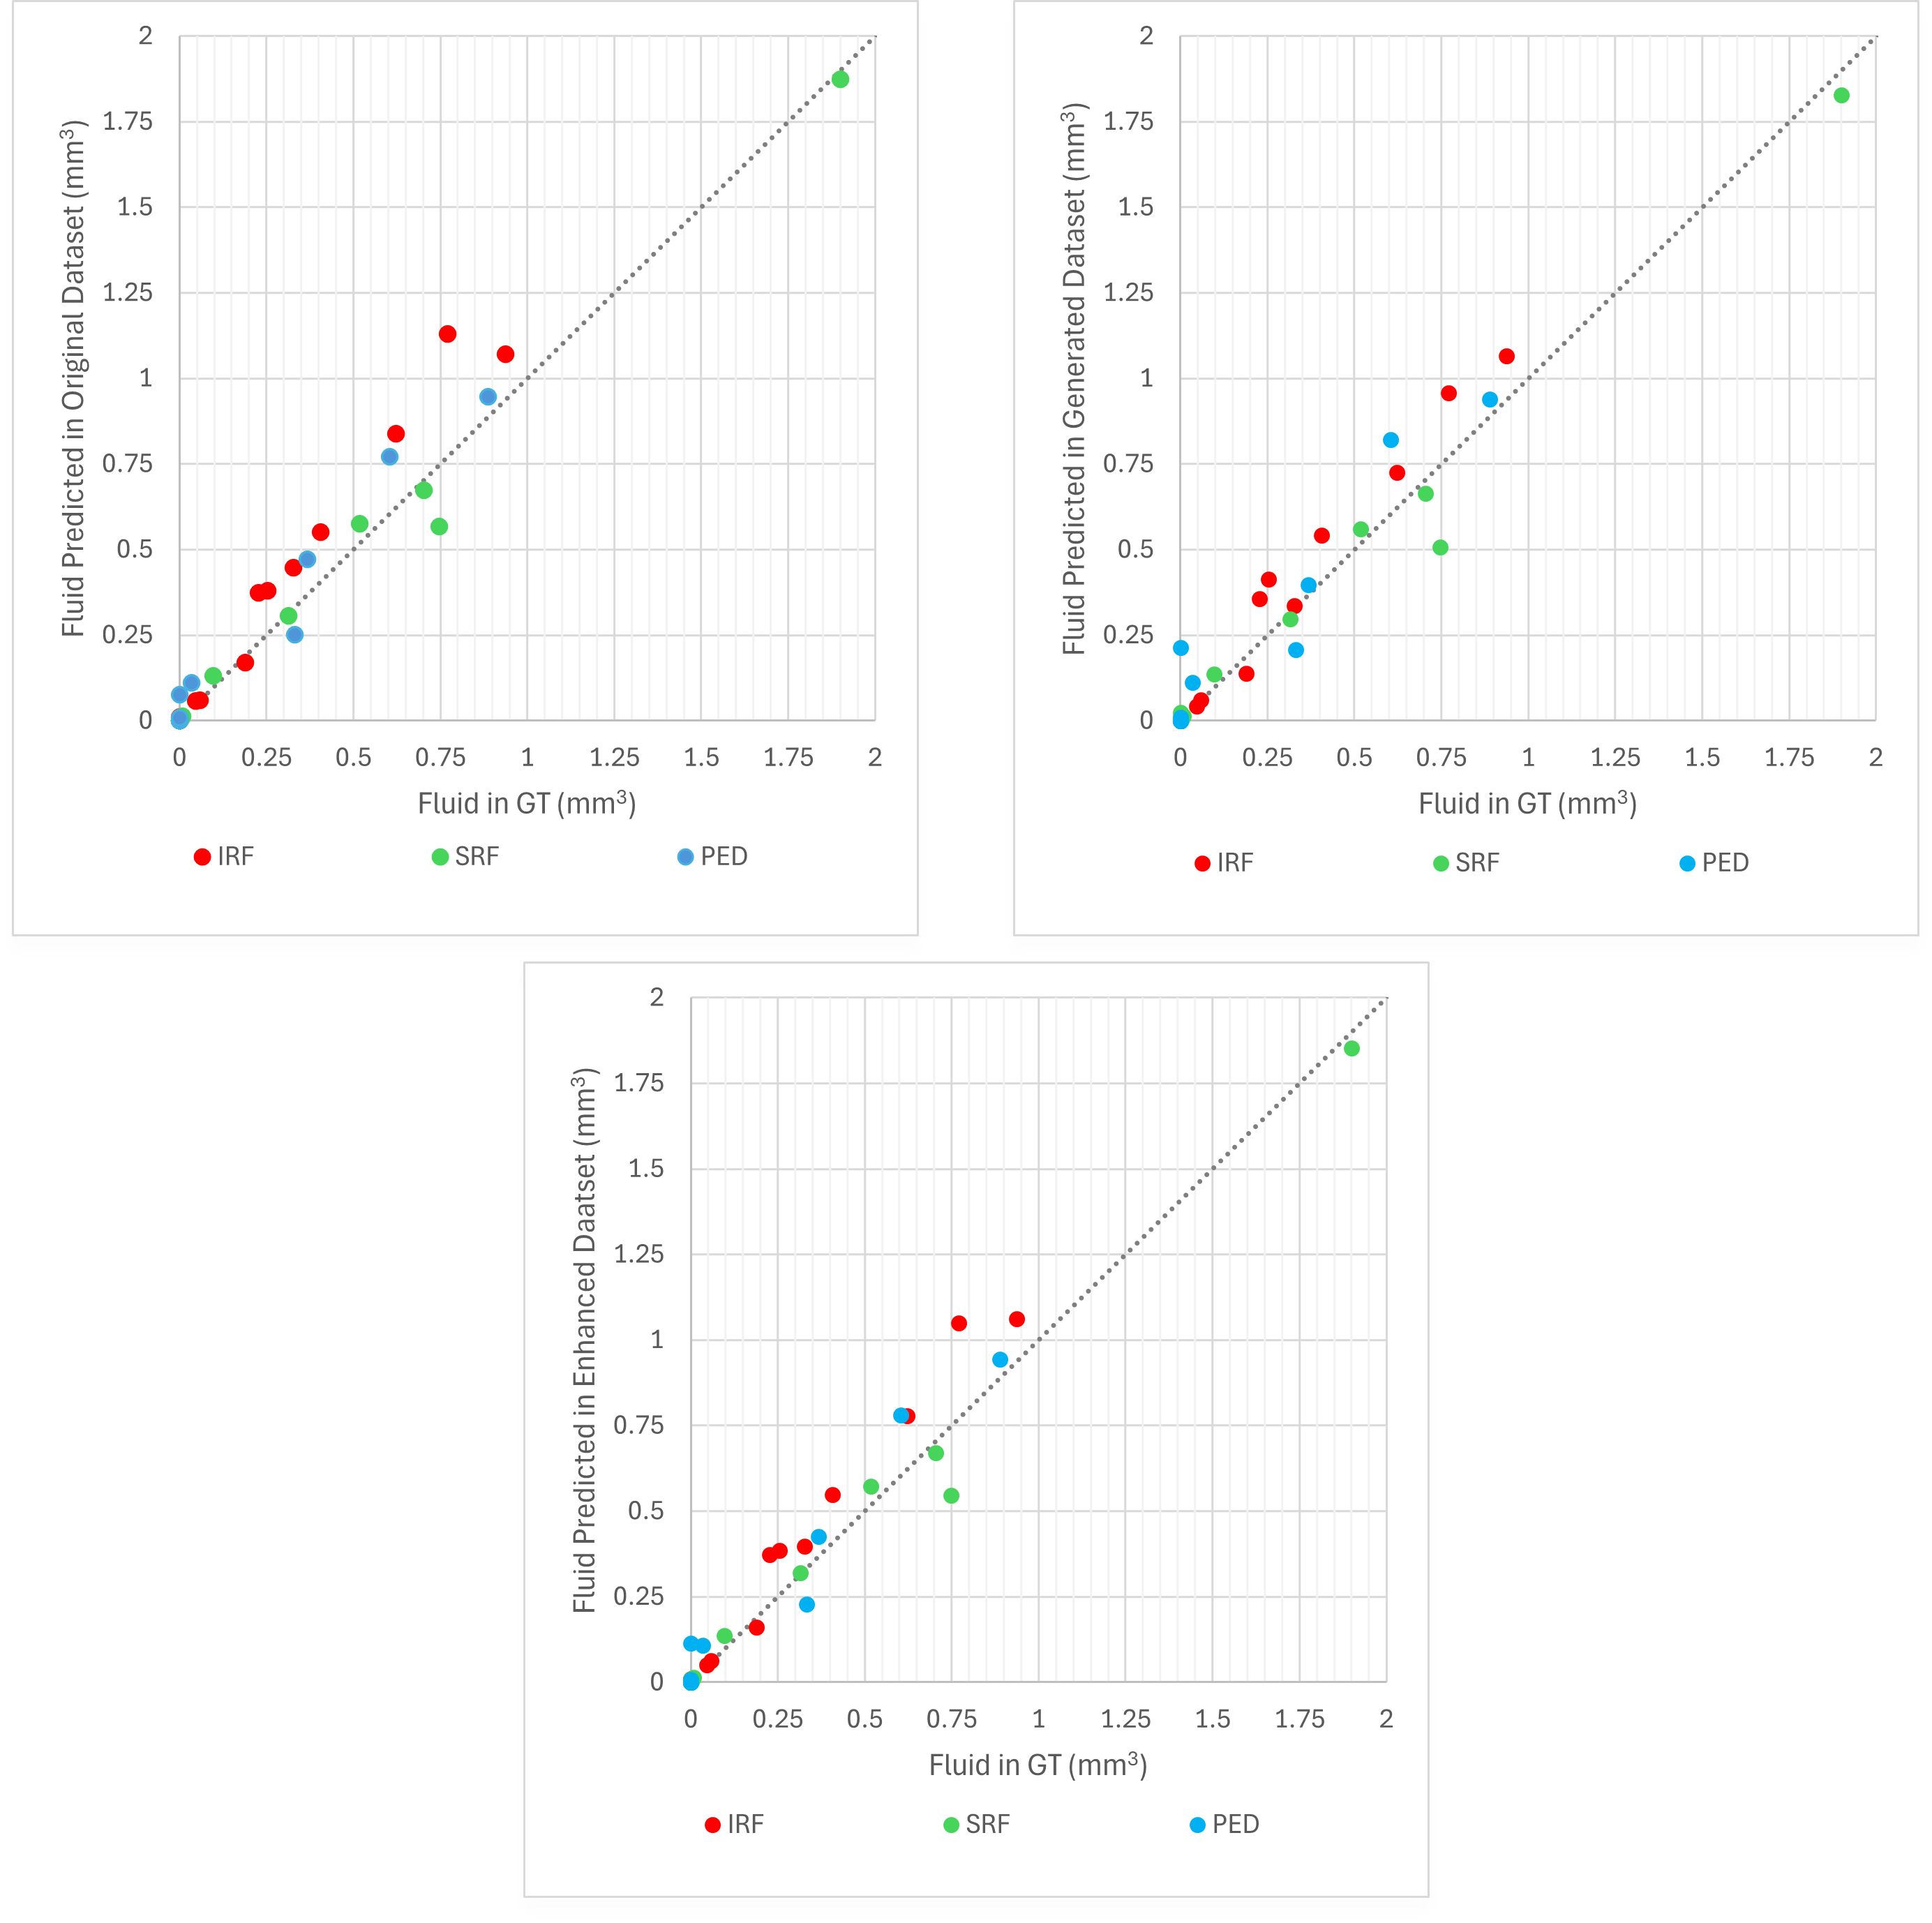
\includegraphics[width=1.0\linewidth]{figures/Experiment6GTvsAll.png}
	\caption{Volume estimated for each fluid in the OCT volumes using the GT masks, compared with the volumes estimated in columns ``P'', ``G'', and ``E''.}
	\label{fig:Experiment6GTvsAll}
\end{figure}

\begin{figure}[!ht]
	\centering	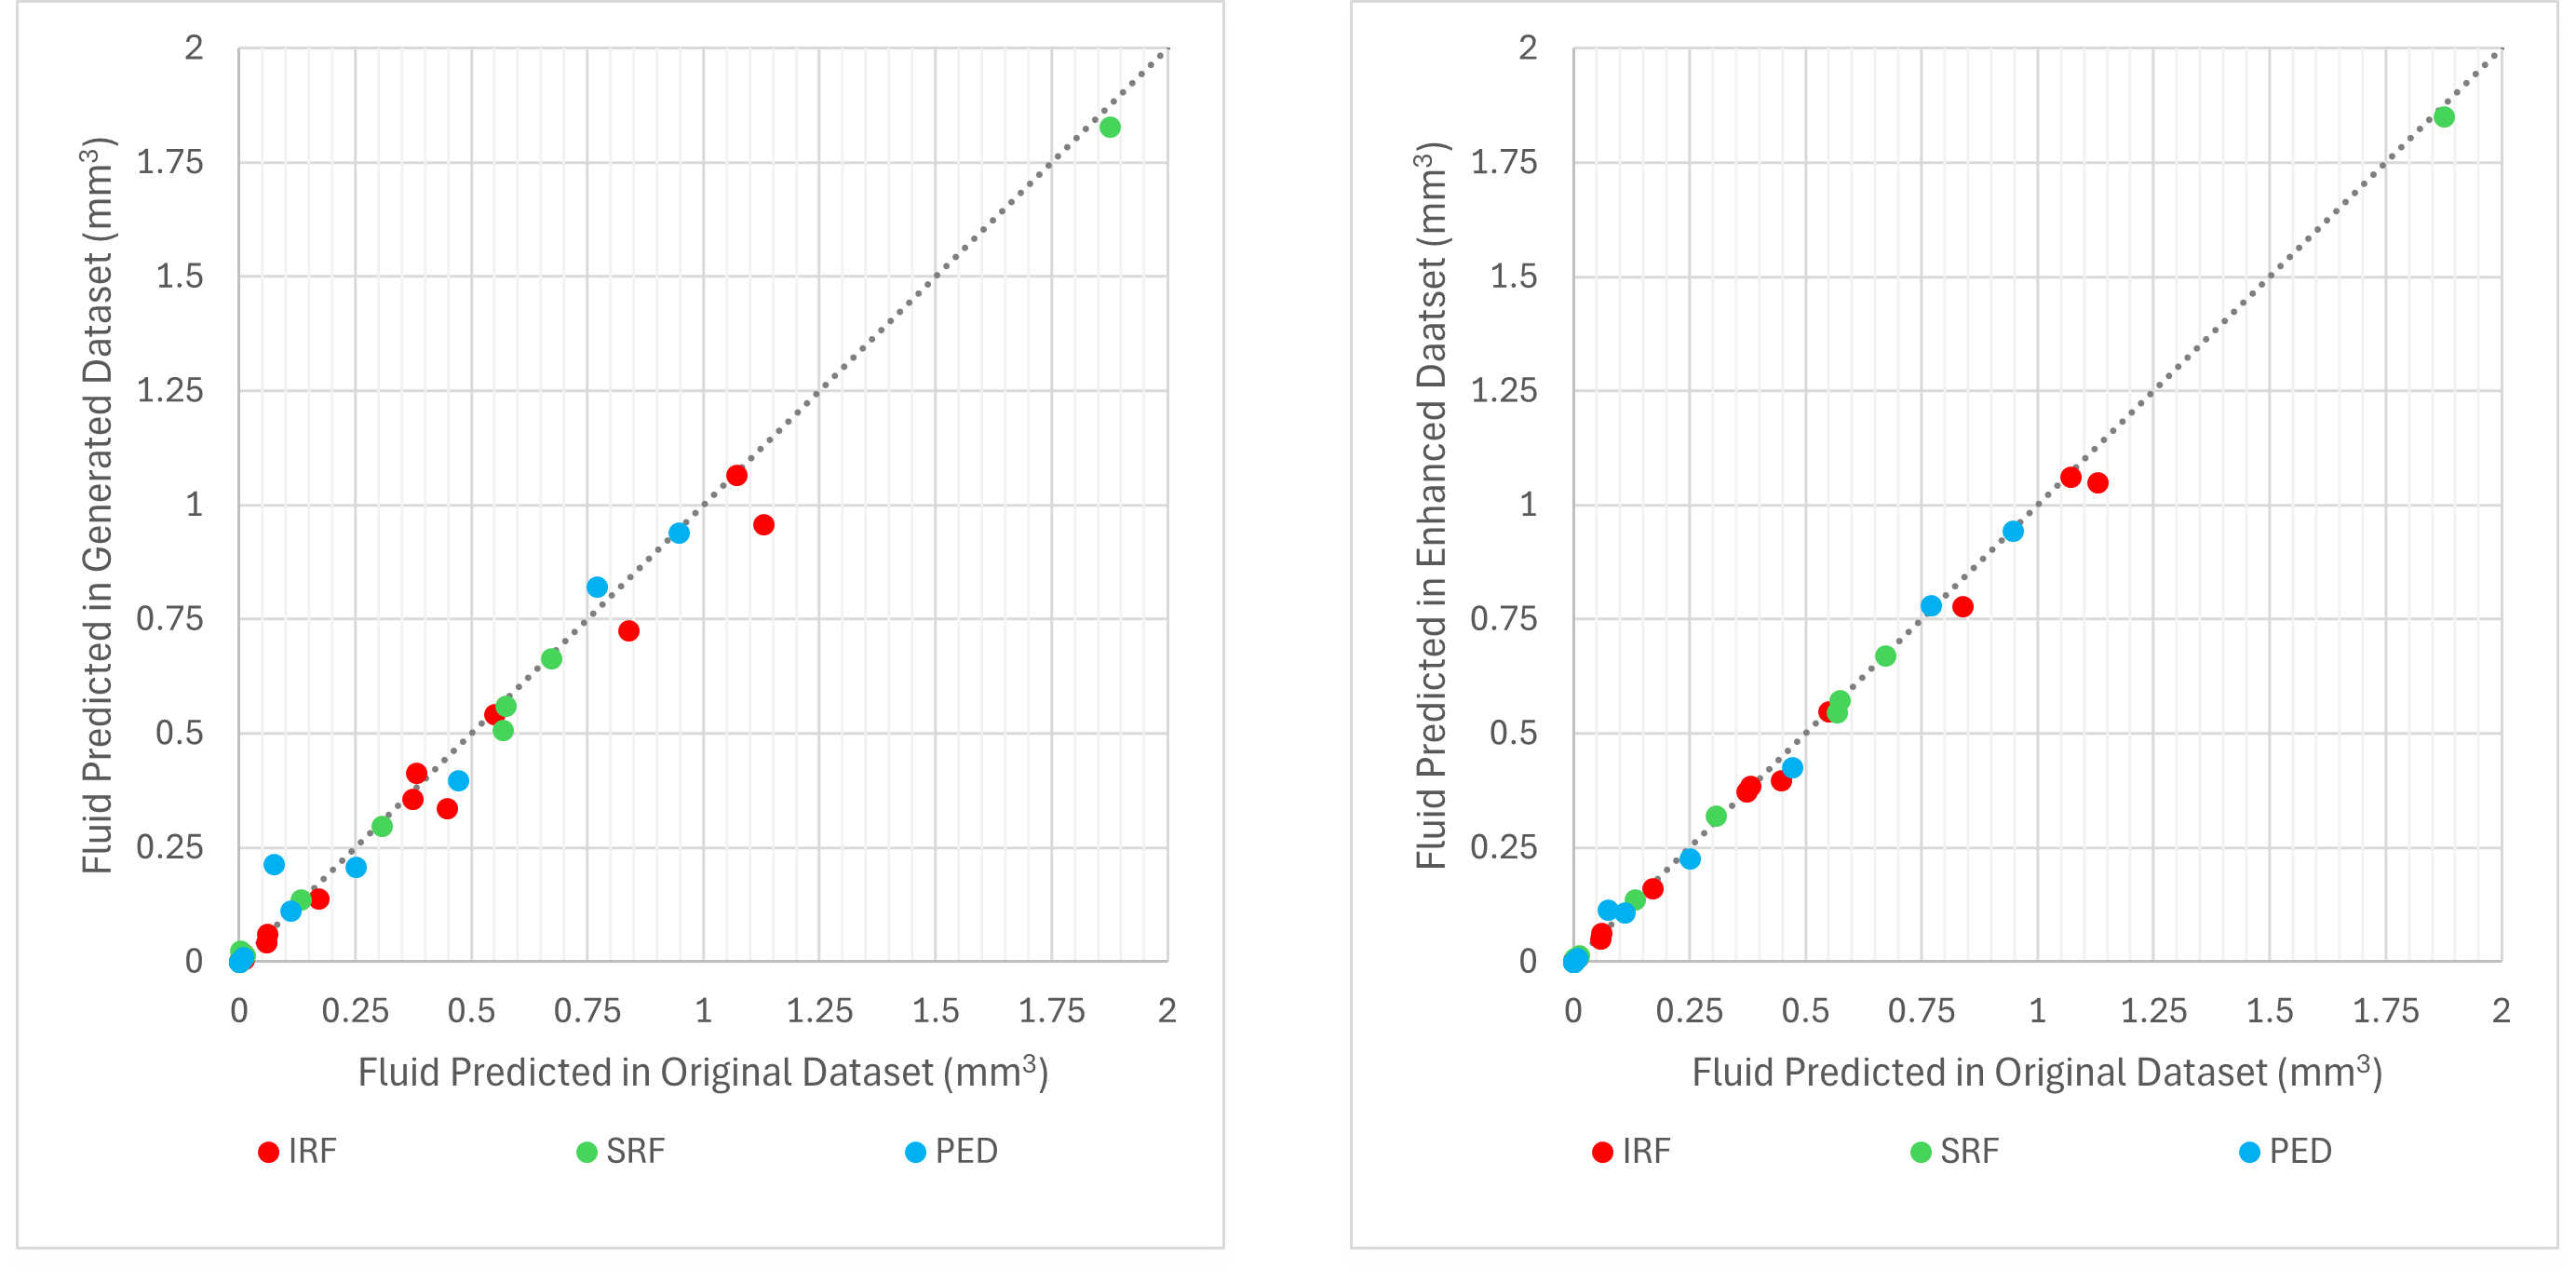
\includegraphics[width=1.0\linewidth]{figures/Experiment6PredictedVsAll.png}
	\caption{Volume estimated for each fluid in the OCT volumes using the masks predicted by the segmentation model compared with the volumes calculated using the masks from columns ``G'' and ``E''.}
	\label{fig:Experiment6PredictedVsAll}
\end{figure}

\begin{figure}[!ht]
	\centering	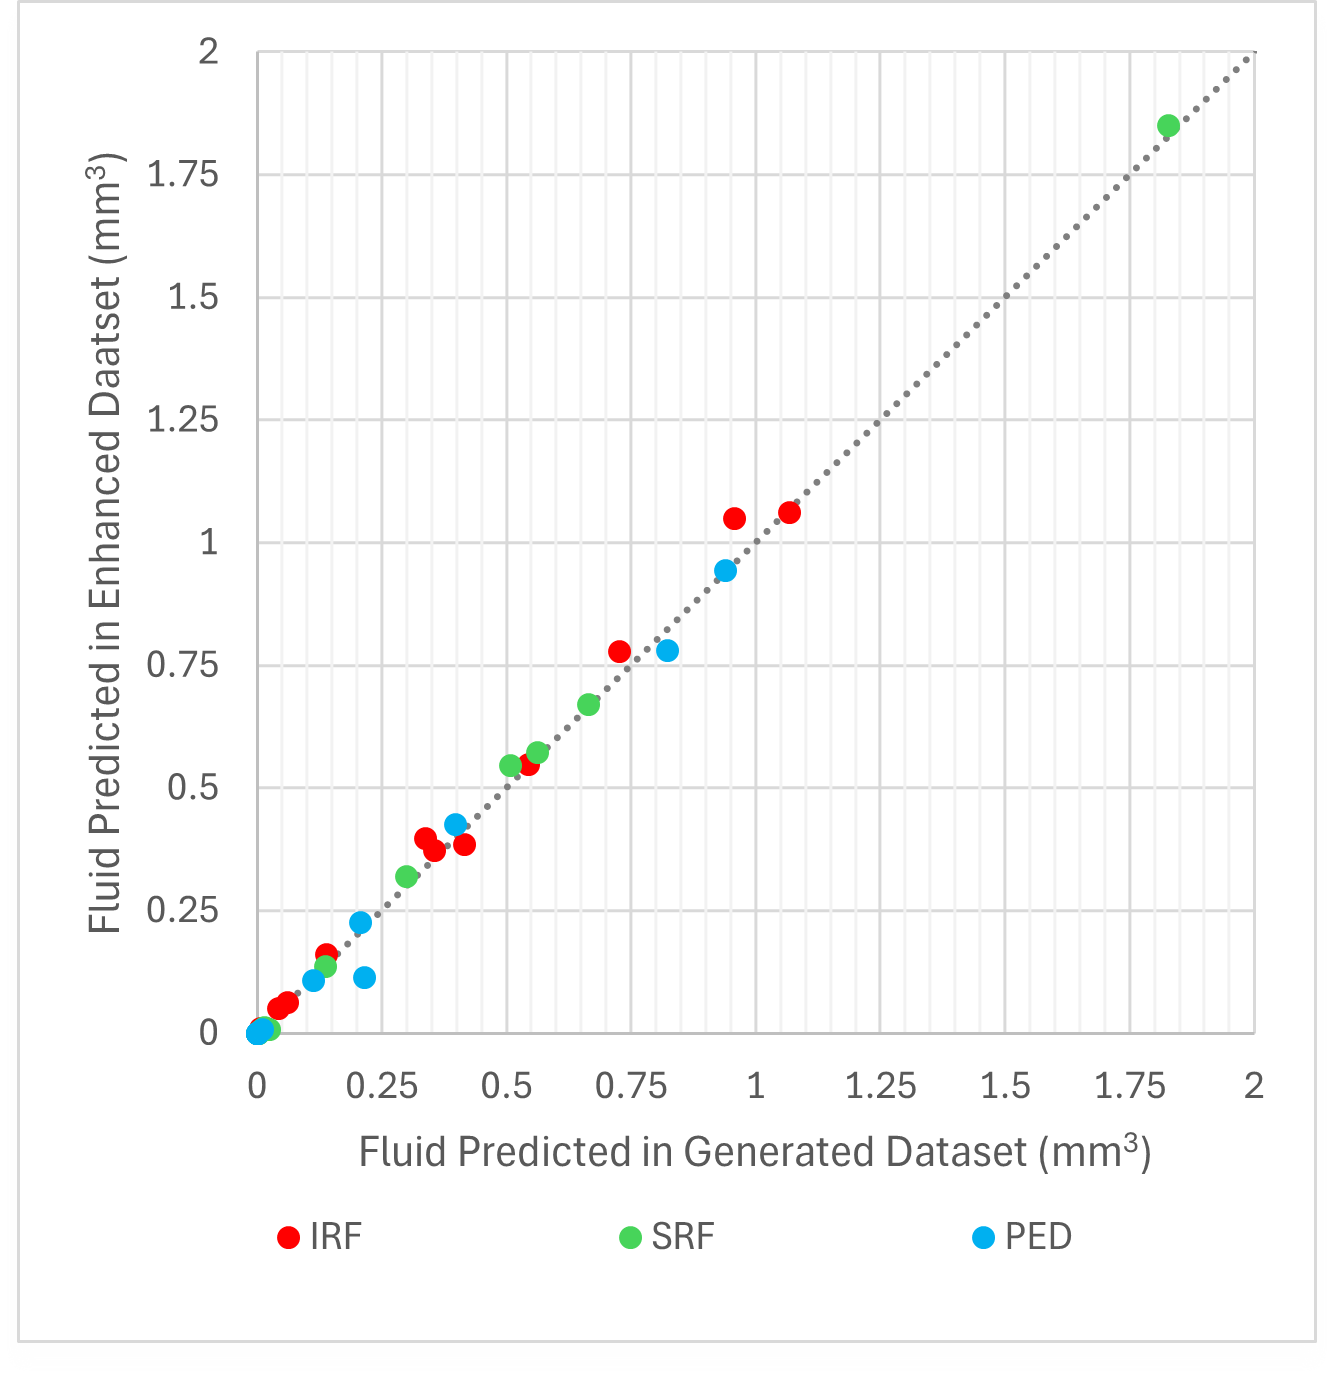
\includegraphics[width=0.50\linewidth]{figures/Experiment6GeneratedVsEnhanced.png}
	\caption{Volume estimated for each fluid in the OCT volumes using the masks predicted by the segmentation model in the generated dataset, compared with the volumes calculated in the enhanced dataset.}
	\label{fig:Experiment6GeneratedVsEnhanced}
\end{figure}

Considering the information exposed in the previous table and figures, many conclusions can be drawn regarding fluid volume estimation. For example, the differences between columns in the estimated fluid volumes, are always larger in IRF. The generation of this fluid was seen in Experiment 3, to be the most difficult, due to the finer details that change in the transitions between consecutive B-scans. Combined with the worse quality in the generated slices, the segmentation of this fluid was also seen to be the most difficult fluid to segment in the volumes from this fold, as shown in Table \ref{tab:Experiment1VsExperiment2}, where the IRF Dice coefficient is lower than in any other fluid. Both aspects significantly influence the estimation of this fluid in the unseen data. 
\par
The SRF presents the smallest differences between columns, as the MAE in this fluid are smaller than in any other fluid. The fluid estimation of SRF benefits from the accurate representation of this fluid in the generated slices, due to its uniform, homogeneous, and predictable characteristics, as seen in Experiment 3. Contrary to IRF, the segmentation model performs exceptionally well in the segmentation of SRF, when compared to the other fluids. Therefore, an accurate representation of the SRF masks is obtained, leading to an accurate fluid estimation.
\par
The estimation of the PED volume appears as an intermediate performance between the other two fluids. The segmentation of this fluid is better than IRF, but worse than PED, while its representation in generated slices is accurate when presented in large regions, but not so good when appearing in small regions. This translates to a smaller deviation between columns when comparing to IRF, but not as good as SRF.
\par
The differences between the columns ``GT'' and ``P'' are inherent to the capability of the segmentation model. This model's capabilities also limit the accuracy of the estimated volumes in the generated and enhanced datasets, as the masks predicted in the generated slices are obtained using this model. Therefore, to understand the effect that generating slices has in total fluid volume estimation, it is important to observe the differences between the ``P'', ``G'', and ``E'' columns. 
\par
The differences between these columns are much smaller than the differences calculated when comparing these results to the GT. This indicates that the fluid estimation is more limited by the segmentation model, than it is by the generated slices. This is particularly true when comparing column ``P'' to column ``E'', as illustrated in Figure \ref{fig:Experiment6PredictedVsAll}. In this figure, most of the points appear close to the gray line, which indicates that the fluid volumes predicted when adding the generated slices are similar to the fluid volumes estimated when predicting the segmentation masks in the original RETOUCH dataset.
\par
To isolate the impact of the generated slices in the fluid estimation, it is more important to look at the differences between the fluids estimated in columns ``P'' and ``G'', as well as Figures \ref{fig:Experiment6PredictedVsAll} and \ref{fig:Experiment6GeneratedVsEnhanced}. By observing this data, it becomes evident the similarity between performances in these datasets. In the SRF fluid estimation, the values are particularly similar, as well as in most cases of PED. However, it is in IRF where the largest differences appear, where the predictions of IRF by the segmentation model are of less quantity in the generated dataset.
\par
As seen in Experiment 3, IRF is the most difficult fluid to generate and attempts to recreate this fluid in intermediate slice, originate structures that do not resemble the IRF fluid. As a result, the segmentation models do not perceive this generated regions as IRF and do not segment them. This trend also seen in Figure \ref{fig:Experiment6PredictedVsAll} in the comparison between the original dataset and the enhanced dataset, where the largest differences appear in the segmentation of IRF, as the segmentation model predicts less fluid in the generated slices. However, since these B-scans are also mixed with original B-scans to form the OCT volume, the resulting differences are less significant.
\par
It is interesting to note that of the three biggest differences in IRF between the columns ``P'' and ``E'', TRAIN016, TRAIN039, and TRAIN048, which are highlighted in Figure \ref{fig:Experiment6PredictedVsAll} as the furthest points from the gray line, are in OCT volumes obtained with the Spectralis device. This trend is related with the larger inter-slice distance in Spectralis than in any other device, which makes it harder to create accurate IRF regions, which is amplified by this fluid's characteristics.
\par
In Table \ref{tab:Experiment6DiceInGeneratedDataset}, the Dice coefficients is calculated for the predicted masks in the generated dataset. These predicted fluid masks are compared to the real GT masks of the equivalent slices. The information shown in this table helps the understanding of which fluids' segmentation and which vendors are the most affected by generating intermediate slices and how these slices are understood by the model.

\begin{table*}[!ht]
	\caption{Comparison in Dice scores for every vendor and fluid in the reserved fold (fold 1), using the best segmentation model to segment the original B-scans and their generated equivalent.}
	\centering
	\resizebox{\textwidth}{!}{\begin{tabular}{|c|c|c|ccc|ccc|ccc|c|c|c|c|}
			\hline
			% Headers
			\multirow{2}{*}{\textbf{OCT Volumes}} &
			\multirow{2}{*}{\textbf{Slices}} &  
			\multirow{2}{*}{\textbf{VF}} & 
			\multicolumn{3}{c|}{\textbf{Cirrus}} & 
			\multicolumn{3}{c|}{\textbf{Spectralis}} & 
			\multicolumn{3}{c|}{\textbf{Topcon}} & 
			\multicolumn{1}{c|}{\multirow{2}{*}{\textbf{IRF}}} & 
			\multirow{2}{*}{\textbf{SRF}} & 
			\multirow{2}{*}{\textbf{PED}} & 
			\multirow{2}{*}{\textbf{Fluid}} \\ \cline{4-12} & & &
			\multicolumn{1}{c}{\textbf{IRF}} & 
			\multicolumn{1}{c}{\textbf{SRF}} & 
			\textbf{\textbf{PED}} & 
			\multicolumn{1}{c}{\textbf{IRF}} & 
			\multicolumn{1}{c}{\textbf{SRF}} & 
			\textbf{PED} & 
			\textbf{IRF} & 
			\textbf{SRF} & 
			\textbf{PED} & 
			\multicolumn{1}{c|}{} & & & \\ 
			
			\hline
			
			\multirow{3}{*}{\textbf{Original}} & All & 1 & 0.852 & 0.918 & 0.934 & 0.645 & 0.821 & 0.852 & 0.818 & 0.929 & 0.755 & 0.799 & 0.905 & 0.841 & 0.742 \\
			
			
			& Fluid & 1 & 0.654 & 0.799 & 0.767 & 0.645 & 0.687 & 0.703 & 0.624 & 0.744 & 0.588 & 0.641 & 0.756 & 0.716 & 0.702 \\
			
			
			& No Fluid & 1 & 0.941 & 0.972 & 0.978 & 0.646 & 0.889 & 0.885 & 0.884 & 0.960 & 0.766 & 0.873 & 0.952 & 0.862 & 0.786 \\	
			
			\hline
			\hline
			
			\multirow{3}{*}{\textbf{Generated}} & All & 1 & 0.740 & 0.896 & 0.903 & 0.307 & 0.707 & 0.850 & 0.763 & 0.870 & 0.726 & 0.671 & 0.850 & 0.816 & 0.627 \\
			
			
			& Fluid & 1 & 0.431 & 0.762 & 0.710 & 0.315 & 0.580 & 0.627 & 0.457 & 0.670 & 0.538 & 0.407 & 0.692 & 0.656 & 0.542 \\
			
			
			& No Fluid & 1 & 0.879 & 0.957 & 0.953 & 0.299 & 0.772 & 0.900 & 0.867 & 0.903 & 0.738 & 0.793 & 0.901 & 0.843 & 0.722 \\
			
			\hline
			
	\end{tabular}}
	\label{tab:Experiment6DiceInGeneratedDataset}
\end{table*}

As expected, the segmentation model performs better in the original dataset, where the structures present in the B-scans are the most similar to those seen in training. Nevertheless, in some metrics, the differences between the generated slices and the original slices is larger than in others.
\par
Regarding the segmentation of slices without fluid, the segmentation model behaves almost similarly to what is seen in the original data in most fluids and vendors. However, there are some exceptions, particularly in IRF and slices from Spectralis. Of all fluids, it is in IRF where the detection of fluid changes the most. This is due to the quality of the generated scans in IRF regions: since this area is harder to predict, the model outputs fluid regions that visually do not resemble IRF, leading the segmentation model to not predict this region as fluid. This particularly affects Spectralis, where the distance between slices is larger, making it harder to interpolate an intermediate slice. For this same reasons, the detection of SRF is affected, particularly due to the poor generation of small SRF regions.
\par
However, it is in the segmentation of slices with fluid where the performances significantly decrease. The segmentation of SRF and PED is not very affected by the generated slices in Cirrus and Topcon when compared to the other fluids. As seen in Experiment 3, the overall shape and characteristics of these fluids are easier to interpolate than IRF, as their structure is constant and homogeneous, with smooth transitions between consecutive slices, particularly in these vendors where the interslice distance is smaller.
\par
Again, the Spectralis generated slices are the ones that result in the largest decrement of segmentation performance in IRF and SRF. As stated previously, the reason behind this poor segmentation is tied to the poor generation of slices when compared to other vendors, which is related to the distance between consecutive slices. The reasons that cause the poor segmentation of the slices with IRF and SRF are the same reasons that lead to the oversegmentation of these fluids in B-scans that do not contain the fluids.
\par
One of the most noticeable outliers of the IRF volume estimation is the Spectralis volume TRAIN039. In Figure \ref{fig:SpectralisTrain039GenerationAndSegmentation}, the segmentation of IRF, as well as two generated slices, are shown.

\begin{figure}[!ht]
	\centering	\includegraphics[width=1.0\linewidth]{figures/SpectralisTrain039GenerationAndSegmentation.png}
	\caption{Example of IRF segmentation in the enhanced volume TRAIN039.}
	\label{fig:SpectralisTrain039GenerationAndSegmentation}
\end{figure}

It is visible in this figure that the second generated slice does not clearly represent the IRF region, as it appears slightly blurred and a large portion of the information does not resemble any structure present in the training images. For this reason, the segmentation model predicts a small area of fluid as IRF in this slice. The predicted area is much smaller than the area of IRF in the surrounding slices. This indicates that the area segmented is not coherent with the information in the surrounding slices, leading to an incorrect predicted fluid volume. The same occurs in the first generated slice of the shown example, but only a smaller portion of the image is unintelligible. 
\par
These two different situations further highlight that the rough transitions particularly affect the slices with small fluid regions, as the model is not capable of predicting which of these regions will appear in the intermediate slice.
\par
In the presented example, a single example of incorrect segmentation due to a poorly generated slice is shown, but multiple examples such as this appear in the predictions made in the mentioned enhanced volume. Accumulating this errors from multiple slices, results in a small total fluid volume than in the predictions made in the original dataset. This explains the decrease in total IRF segmented in the enhanced Spectralis volume when compared to the predictions in the original volume, as seen in Table \ref{tab:FluidVolumesExperiment6}.
\par
Figure \ref{fig:CirrusTrain012GenerationAndSegmentation} shows the segmentation of large SRF and PED volumes in the enhanced Cirrus TRAIN012 volume.

\begin{figure}[!ht]
	\centering	\includegraphics[width=1.0\linewidth]{figures/CirrusTrain012GenerationAndSegmentation.png}
	\caption{Example of SRF and PED segmentation in the enhanced volume TRAIN012.}
	\label{fig:CirrusTrain012GenerationAndSegmentation}
\end{figure}

In the shown generated images, the overall structure of the SRF and PED fluids is easier to accurately represent in the intermediate slices. Not only the transitions are smoother due to the smaller inter-slice distance in the Cirrus volumes, but also because of their homogeneous and regular shapes. Small artifacts that are seen in the GT slices are not represented in the intermediate slice, as they are unpredictable.
\par
As the generated fluid regions show the appearance that is characteristics of the true fluid regions in the original scans that compose the RETOUCH dataset, its segmentation is visually similar to the segmentation performed in the surrounding slices, which resemble the GT masks of the surrounding slices. 
\par
This example shows an accurate segmentation and generation of an enhanced OCT volume. This is a sample of segmentation and generation in the TRAIN012 volume, but most slices are segmented and generated as accurately as the shown example. This results in predicted fluid volumes that are similar to those estimated with the GT masks and with the predicted masks in the unchanged OCT volume.